\documentclass[final,index,idxtotoc,fleqn,USenglish,pdftex,twoside,a4paper,bibtotoc,abstracton,headsepline,openright]{scrreprt}
\usepackage{color}
\usepackage{xspace}
\usepackage{makeidx}
\usepackage[final]{graphicx}
\usepackage[USenglish, german]{babel}
\usepackage[final]{cvsserver} % [rcsinfo] 
\usepackage{varioref}
\usepackage{prooftree}
\usepackage{holz}
\usepackage{pdflscape}
 %
%%%%%%%%%%%%%%%%%%%%%%%%%%%%%
%% local macro definitions %%
%%%%%%%%%%%%%%%%%%%%%%%%%%%%%
\newcommand{\zcomment}[1]{#1}
%%macro \zcomment 1
\newcommand{\unix}{Unix\xspace}
\newcommand{\posix}{POSIX\xspace}
\newcommand{\holz}{HOL-Z\xspace}
\newcommand{\cvscmd}[1]{\textsf{#1}\index{#1@\textsf{#1}}} % all CVS commands like checkin
\newcommand{\unixcmd}[1]{\texttt{#1}\index{#1@\textsf{#1}}}    % all Posix/Unix commands like mv, cp
 
\newcommand{\susv}{SUSV\xspace}
\newcommand{\pplus}{+}
\newcommand{\front}{\Zpreop{front}}
\newcommand{\isdirin}{\Zinrel{is\_dir\_in}}
\newcommand{\isfilein}{\Zinrel{is\_file\_in}}
\newcommand{\isin}{\Zinrel{is\_in}}
\newcommand{\aim}[1]{\hfill\\$\Longrightarrow$ #1}
\newcommand{\bindsto}{\mapsto}
\newcommand{\rbac}{RBAC\xspace}

\newenvironment{doc}[1]{}{}
\rcsInfo $Id: arch.tex,v 1.139 2003/12/04 15:03:05 brucker Exp $
\publishers{Institut f{\"u}r Informatik, Universit{\"a}t Freiburg\\
           Georg--K{\"o}hler--Allee 52, 79110 Freiburg, Germany}
\title{A CVS-Server Security Architecture \\ --- \\ Concepts and Formal Analysis}
\author{\href{http://www.brucker.ch}{Achim D. Brucker}
  \and 
  \href{http://www.informatik.uni-freiburg.de/~rittinge}{Frank Rittinger}
  \and 
  \href{http://www.informatik.uni-freiburg.de/~wolff}{Burkhart Wolff}
}
\subject{Technical Report $182$\\
 Updated Version: 2003-12-04}
\publishers{Institut f{\"u}r Informatik \\
  Albert--Ludwigs--Universit{\"a}t Freiburg \\
  Georges-K{\"o}hler-Allee 52 \\
  D-79110 Freiburg, Germany \\
  Tel: +49 (0)761 203-8240, Fax: +49 (0)761 203-8242 \\[1.1\baselineskip]
  \texttt{\small\{brucker,rittinge,wolff\}@informatik.uni-freiburg.de} \\
  \texttt{\small http://www.informatik.uni-freiburg.de/\char'176{}\{brucker,rittinge,wolff\}}
}
%%
%% setup for hyperref: 
\hypersetup{%%
  pdftitle={A CV security architecture},
  pdfauthor={(c) 2001,2002,2003,2004 Achim D. Brucker and Frank Rittinger and Burhart Wolff},
  pdfsubject={},
  pdfkeywords={CVS, security architecture},
  colorlinks=false,
  draft=false,
  backref=none,
  bookmarksnumbered=true,}
%%
\uppertitleback{\textbf{Acknowledgements:}\\ We would like to thank Nicole Rauch (Uni
  Kaiserslautern) for many valuable comments on a draft version of this paper.
  Harald Hiss provided in his Studienarbeit most of the consistency proof-work
  done in Chapter~\ref{chap:verification}. Stefan Friedrich also made comments
  on an early version of the report and contributed to discussions and proofs to
  the library of HOL-Z.}

\lowertitleback{The latest version of this technical report, of the CVS-server
  specification, and the proof scripts can be found in the example section of
  the HOL-Z distribution, which is available at:
  \url{http://wailoa.informatik.uni-freiburg.de/holz/}\\
  The underlying implementation can be downloaded at:
  \url{http://www.informatik.uni-freiburg.de/~softech}}
\renewcommand{\sectfont}{\rmfamily\bfseries} %% no sffamily
\makeindex
\begin{document}
\pagestyle{empty}
\selectlanguage{USenglish} 
\maketitle 
%%%%%%%%%%%%%%%%%%%%%%%%%
%% Abstract            %%
%%%%%%%%%%%%%%%%%%%%%%%%%  
\begin{abstract}
  We present a secure architecture of a CVS-server, its implementation (i.e.\ 
  mainly its configuration) and its formal analysis. Our CVS-server uses
  cvsauth~\cite{vogt:cvsauth:2001}, that provides protection of passwords and
  protection of some internal data of the CVS repository. In contrast to other
  (security oriented) CVS-architectures, our approach makes it possible to
  CVS-server on an open filesystem, i.e.\ a filesystem where users can have
  direct access both by CVS-commands and by standard UNIX/POSIX commands such as
  \unixcmd{mv}. A key feature of our implementation is that it enforces a
  particular access control model, namely role-based access control (RBAC).
  
  For our secure architecture of the CVS-server, we provide a formal
  specification and security analysis. This is based on a refinement, mapping a
  system architecture on an implementation architecture abstractly describing
  CVS in our implementation. The system architecture describes the abstract
  system operations including the desired access control model RBAC and serves
  as backbone to describe overall security requirements formally. The
  implementation architecture --- to be seen as an abstract program ---
  describes the security mechanisms on the UNIX/POSIX filesystem level, namely
  discretionary access control (DAC).
 
  The purpose of the formal analysis of the secure CVS-server architecture is
  twofold: First, we describe our implementation, in particular the access
  control for our open architecture. Second, we provide a method to analyze
  formally security implementations (beyond the code level) for realistic
  applications in terms of off-the-shelf security technologies.
  
  \begin{labeling}{\textbf{Keywords:}}
    \item[\textbf{Keywords:}] security, formal methods, software architecture, 
                              Concurrent Versions System (CVS), Z, refinement 
  \end{labeling}
\end{abstract}
%%%%%%%%%%%%%%%%%%%%%%%%%
%% Table of Contents   %%
%%%%%%%%%%%%%%%%%%%%%%%%%
\tableofcontents 
\pdfbookmark[0]{Contents}{toc}
% \listoffixmes
%%
\pagestyle{headings}

\rcsInfo $Id: intro.tex,v 1.11 2003/12/04 15:03:06 brucker Exp $

\chapter{Introduction}\label{chapter:introduction}
These days, the \emph{Concurrent Versions System}\index{Concurrent
  Versions System|see{CVS}}\index{CVS} (CVS) is a widely used tool for
version management in many industrial software development projects
and plays a key role in open source projects usually performed by
highly distributed
teams~\cite{cederqvist.ea:cvs:2000,fogel:cvs:1999,cvshome:2001}.  CVS
provides a central data base (the \emph{repository}\index{repository})
and means to synchronize local partial copies (the \emph{working
  copies}\index{working copy}) and their local modifications with the
repository\index{repository}. CVS can be accessed via a network; this
requires a security architecture establishing authentication, access
control and non-repudiation.  A further complication of the CVS
security architecture stems from the fact that the administration of
authentication and access control is done via CVS itself; i.e.\ the
relevant data is accessed and modified via standard CVS operations
and, thus, access to objects may change dynamically.
 
The current standard CVS-server distribution (based on the
\texttt{pserver}-protocol)\index{pserver@\texttt{pserver}} is known to
be quite insecure: since passwords are not encrypted during
communication, usual password-sniffing attacks can be applied;
moreover, a bug in some CVS-operations can allow an arbitrary user to
modify the password authentication table.  Further, any CVS user (with
write access) can execute any program on a server with the userid he
is authenticated to. This means he can send himself a command shell.
Via buffer-overflow attacks, there is the inherent danger that the
CVS-server can be crashed leaving a command shell under root
permissions.  Additionally, the repository in itself is not protected
against direct user manipulations via file system operations.

Moreover, the current CVS-server distribution inherits the usual \unix{}
permission\index{Unix!permission} concept --- this may be too low-level and
inadequate to cope with the demands of many user-groups and their work
organization. In particular, we found it useful to provide a special
configuration of the CVS-server that enforces a hierarchical \emph{role based
  access control}\index{role based access model} model as described
in~\cite{sandhu.ea:role-based:1996}. This model associates to users one or more
\emph{roles} (e.g.\ project supervisor, test engineer, programmer, project
member, etc) that are organized in a partial order. Further, \emph{permissions}
are associated to objects in the repository; a user may authenticate for a
particular role in order to get appropriate permissions for object access.

In order to install the current CVS-server in security conscious way,
the traditional architecture requires the server to run on a
secured machine that has exclusive access to an own file-system
hosting the repository. This \emph{closed architecture} has a number
of administrative and technical costs (additional hardware,
efficiency).

In order to overcome some of these problems, we propose a number of improvements
of the standard CVS-server, either on the level of its implementation (via
patches), its configurations (i.e.\ the file system, including the initial state
of the repository; this extends to group-tables, file permissions, scripts
started when check in or check out data into the repository) or its architecture
(i.e.\ the particular setup of a cvs-server and its configuration in a network).
Our first main goal of our work is to provide a particular configuration of
CVS-server that enforces a role-based access control security policy. Our second
main goal is to develop an \emph{open} CVS-server architecture, where the
repository is part of the usual shared file-system of an intranet and the server
a regular process on some machine in it. While an open architecture has
undoubtedly a number of advantages, the correctness and trustworthiness of the
security mechanisms becomes a major concern.  In order to meet these concerns,
we will present in this paper formal models and an analysis of the open
CVS-server security architecture.


Our contribution in this paper is fivefold:
\begin{enumerate}
\item We provide a formal model of the CVS-server \emph{system
    architecture}\index{system architecture}\index{architecture!system}, that
  provides a \emph{hierarchical} role based access control model for a fixed
  preconceived hierarchy of CVS-roles. Our CVS-server security architecture
  model contains \cvscmd{checkout} and \cvscmd{checkin} operations of CVS with respect to the
  access control policy resulting from the CVS-role hierarchy.
\item We provide a formal model of the \emph{implementation
    architecture}\index{implementation
    architecture}\index{architecture!implementation} based on the UNIX/POSIX
  file-systems and its security mechanisms.  Methodologically, the
  implementation architecture is a refinement of the system architecture.
\item We provide semi-formal and formal (machine-assisted) proofs for the
  consistency of the specification and for the refinement.  Moreover, we provide
  proofs for the security properties both on the system and the implementation
  level of the architecture.  The proofs take into account that on the
  implementation level UNIX-operations like \unixcmd{cd}, \unixcmd{chmod},
  \unixcmd{chown} can be used within attacks.
\item We provide insight into the limits of refinement based,
  well-known abstraction techniques for the security analysis of
  real-world applications.  In particular, realistic security analysis
  involves the formal analysis of \emph{attacks against the
    implementation}; thus, models have to provide sufficient detail of
  the security mechanisms of the implementation architecture.
\item We provide a particular \emph{configuration} of our CVS-server
  architecture, that implements our open, intranet compliant architecture. Our
  implementation is based on standard CVS extended by \emph{cvsauth}\index{cvsauth} that
  incorporates SSL/TSL-support~\cite{itef:rfc2246:1999}\index{secure socket
    layer|see{SSL}}\index{SSL} for secure communication of remote CVS access.
\end{enumerate}

The overall benefit of our implemented architecture consists in
security against most of the known attacks as listed above: Password
sniffing is prevented by encryption, gaining root access by
cvs-command attacks is prohibited, the danger of gaining root access
by buffer-overflow attacks is limited to the authentication phase,
which is the only remaining phase where the server runs under root.
Additionally, administration of our CVS-server architecture is
independent from system administration (except during initialization).
And, last but not least, our open CVS-server can run on an arbitrary
machine (say, the file server) with standard access to the
file-system, which has become possible due to our formal modeling and
analysis.
   
As formal specification language, we use the Z-Notation~\cite{iso:z:2000} 
for specifying our model. For theorem-proving, we compile our
\LaTeX-based specification via a own translator to 
HOL-Z~\cite{kolyang.ea:hol:96,brucker.ea:hol-z:2002} based on
Isabelle98~\cite{paulson:isabelle:1994,nipkow.ea:isabelle:2002}.  Since Z is typed set-theory
and as such semantically equivalent to higher-order logic (HOL; modulo
minor differences w.r.t.\ polymorphism; see~\cite{santen:HOL:1998} for
details.), we treat Z as a mere syntactic front-end to HOL\@. As such,
Z offers a compact syntax geared towards data-modeling, which is
normed~\cite{iso:z:2000} and for which many excellent text-books for
software-engineers are available. For Z, an excellent \LaTeX-based
literate specification environment is available (\cite{zeta}; with own
type-checker etc.).

We proceeds as follows: After a discussion of our notion of
architecture and architectural refinement, we come to the core
chapters of this paper: the system architecture model (or: abstract
layer of the refinement), the \unix{} model as infrastructure for the
implementation architecture, and the implementation architecture
itself. Further, we describe the refinement relation between these
two, the security properties formalizable at the different layers and
their analysis.

%%% Local Variables:
%%% TeX-master: "arch"
%%% fill-column:80
%%% x-symbol-8bits:nil
%%% End:

\rcsInfo $Id: cvs-server.tex,v 1.12 2002/12/28 18:43:33 brucker Exp $

\chapter{Excursion: Modeling the Architectures of CVS-server}
In this section, we will discuss several alternatives of CVS-server\index{CVS-server}
architectures, namely the (traditional) closed CVS-server architecture and our
proposed open CVS-server architecture.  The closed CVS-server architecture
naturally arises, if one wishes to install a CVS repository ``out-of-the-box'' but
wants to prevent that users may directly access and destroy the repository;
moreover, if one wants to implement a hierarchical access structure within the
elements of the repository. As already mentioned, our ``open approach'' attempts
to overcome some limitations of the ``closed approach'' at the price of
\emph{potentially} higher security risks - whose formal proof of irrelevance is
the ultimate goal of this paper. The purpose of this section is to give a wider,
architectural perspective of the system than the data-model used and analyzed in
the next sections.

In order to describe the \emph{architecture}\index{architecture} of a
system, it is common practice to use diagrams for this purpose,
enriched by outlines of a formal specification in a behavioral
specification language. Following the approaches of
Garlan~\cite{garlan:arch:93,shaw:arch:96}, architectures are composed
by \emph{components}\index{component} and
\emph{connectors}\index{connector}. Components are computational units
that interact via connectors with each other; connectors can be remote
procedure calls, communication protocols or access to shared
variables. Garlan proposes a semantics for these notions in terms of
the process-algebra CSP~\cite{roscoe:csp:98}\index{CSP}. As a basis for
discussions over the architecture of CVS--server, we will roughly
follow this approach; in this setting, components are just processes,
while connectors are also processes or particular parallel operators
of CSP.

The \emph{closed CVS-server architecture}\index{CVS-server!closed}
is easily depicted as in Fig.~\ref{fig:overview1}.
  \begin{figure}
    \center
      \scalebox{0.5}{\input{pics/arch_overview}}
    \caption{An overview of the standard security architecture.\label{fig:overview1}}
  \end{figure}
In this architecture, we have:
\begin{itemize}
 \item two types of components, (one family of client components, one CVS-server).
 \item client components have two distinct roles (stduser, cvsadmin).
   The standard user gets access along a predefined hierarchy of
   access control rights for the commands \cvscmd{checkin} and
   \cvscmd{checkout}.  The cvs-administrator may additionally change
   the state of the repository by changing the access permissions
   within the repository. The authentication\index{authentication} is
   done in this model by the CVS \cvscmd{login} operation.
 \item the underlying assumption that the repository is internal 
       in a particular closed machine with the repository inside.     
 \item no direct access to the repository by the user,
       only indirect access to the repository by the cvs administrator.
 \item direct access to the repository for the administrator.
\end{itemize}
  \begin{figure}
    \center
      \scalebox{0.5}{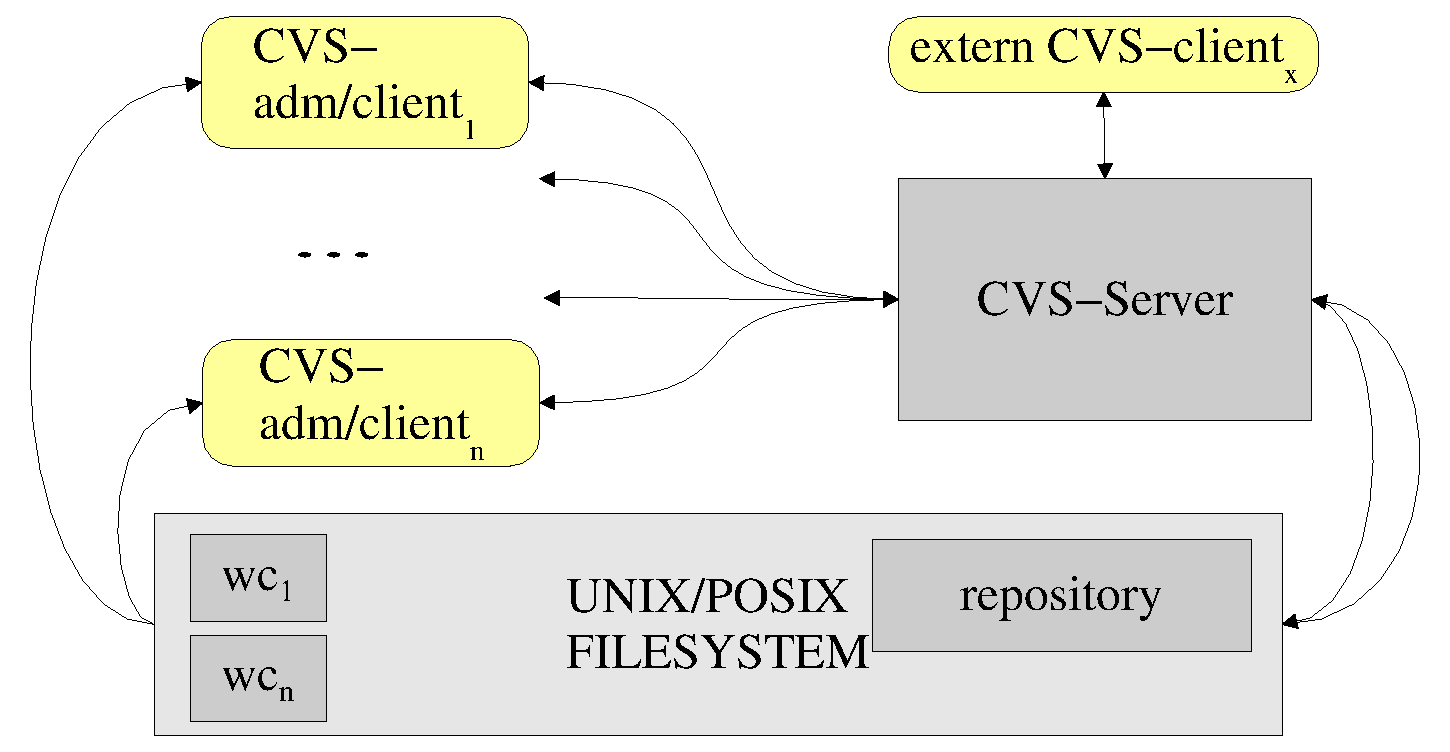
\includegraphics{pics/arch_overview3}}
      \caption{An overview of the open security architecture.\label{fig:overview3}}
  \end{figure}
  In contrast the the setting discussed above, our \emph{open
    CVS-server architecture}\index{CVS-server!open} (see
  Fig.~\ref{fig:overview3}) is depicted as follows:
\begin{itemize}
\item three types components (a family of clients, a server, and the
  UNIX-filesystem).
\item clients may have one of four roles ({stduser, cvsadmin} $\cross$
  {user, sysadmin}).
\item the repository and the working copies are parts of the same
  underlying filesystem; this captures exactly the implementation
  reality.
\item users and CVS-server have in principle equal rights to access the
  filesystem.
\item direct access to the repository for the administrator
\item the architectural view does not capture the fact that the users
  should have \emph{different} access to the elements of the
  repository.
\end{itemize}    
One could add a further type of client into this architecture, namely
the ``externclient'' that has no direct access to the file system;
this represents users that connect to the server without having an
account in the local network the server operates in. But since this
type of client represents a special case of the clients considered
here (and can thus not introduce new complications with respect to
security), we omit it for simplicity reasons.  So far, we have
presented architectures as a graph of of components (belonging to
certain types), that have ``roles'' and that interact along
``connectors'' (depicted as arcs in the diagrams, whose exact nature
is left open.  A more formal description of the model that captures
the communication events in more detail may look as shown in
Fig.~\ref{fig:overview4}.
  \begin{figure}
    \center 
      \scalebox{0.5}{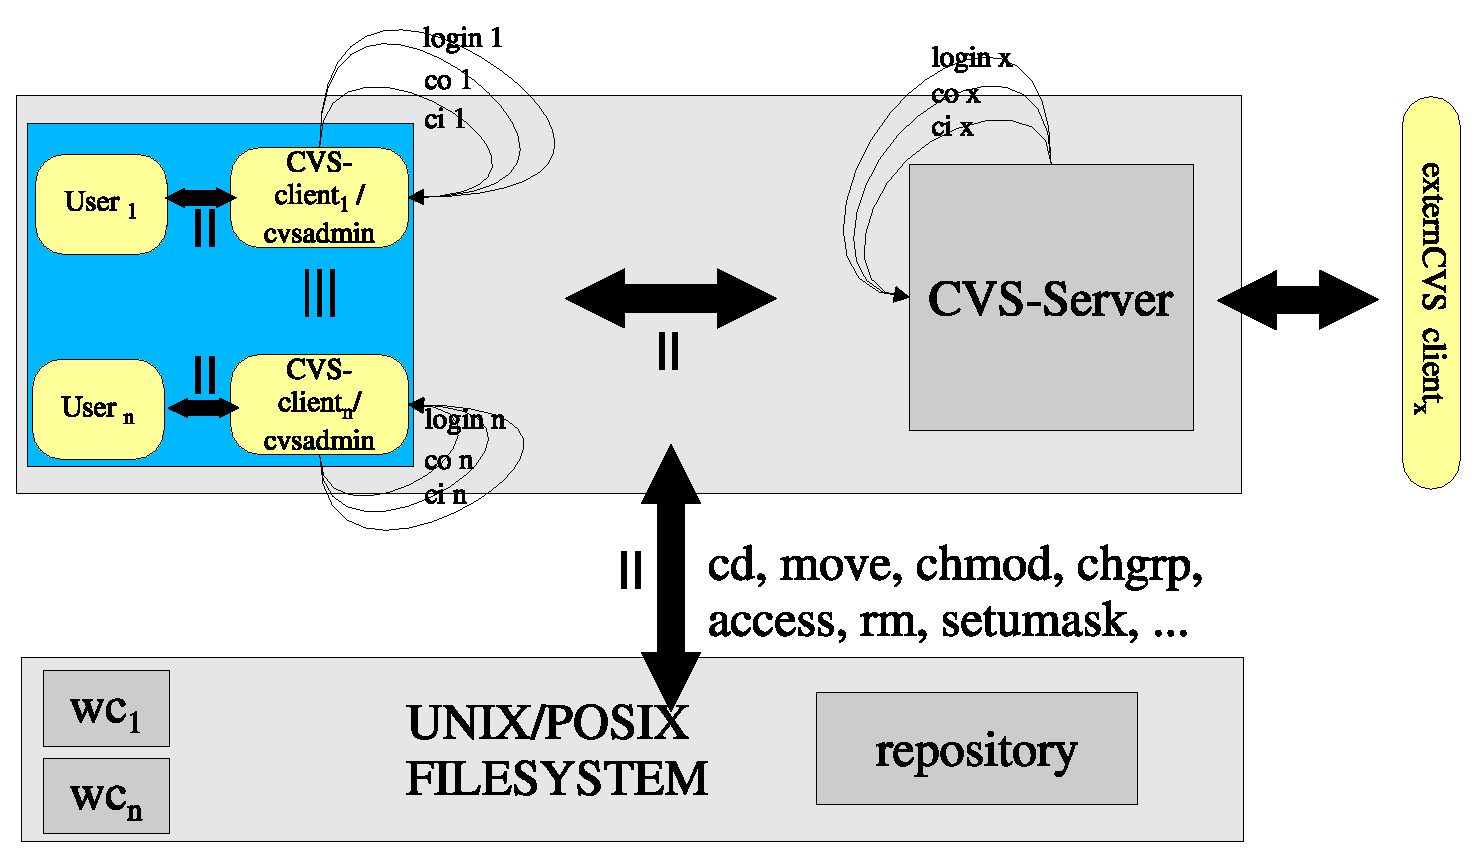
\includegraphics{pics/arch_overview4}}
    \caption{Communication in the open security architecture.\label{fig:overview4}}
  \end{figure}
  Here, we have a collection of user-side CVS-client processes, that may perform
  \cvscmd{cvs\_login}, \cvscmd{cvs\_ci} (checkin), \cvscmd{cvs\_co} (checkout),
  \unixcmd{cd}, \unixcmd{read}, \unixcmd{write}, \unixcmd{mv}, \unixcmd{mkdir},
  \unixcmd{rmdir}, \unixcmd{rm}, \unixcmd{setumask}, \unixcmd{chgrp} and
  \unixcmd{chmod} commands (parameterized in this very simple behavioral model
  just by their user ID $uid$). We assume one particular uid ``root''.  Further,
  we assume a collection of roles and authentication for them.  Now our formal
  architecture model is defined as a collection of interleaved processes that can be
  stated as follows:
\begin{cspverb}
   CLIENT(uid) = |~| role:ROLE,pwd:PWD @ 
                     cvs_login!uid!role!pwd -> CLIENT(uid) |~| 
                     cvs_ci!uid             -> CLIENT(uid) |~|  
                     cvs_co!uid             -> CLIENT(uid) |~|  
                     cd!uid                 -> CLIENT(uid) |~|  
                     read!uid               -> CLIENT(uid) |~|  
                     write!uid              -> CLIENT(uid) |~|  
                     mv!uid                 -> CLIENT(uid) |~| 
                     mkdir!uid              -> CLIENT(uid) |~|  
                     rmdir!uid              -> CLIENT(uid) |~|  
                     rm!uid                 -> CLIENT(uid) |~| 
                     setumask!uid           -> CLIENT(uid) |~|  
                     chgrp!uid              -> CLIENT(uid) |~|  
                     chmod!uid              -> CLIENT(uid) 

   CLIENTS = ||| u:UID @ login!uid -> CLIENT(uid)
\end{cspverb}
In the model above, we allow the user to apply for arbitrary roles ---
later, more refined models of the CVS-server will refuse traces
where the clients do not apply appropriate authentication, but
here we concentrate just on the possible communications. However,
we require that any client process starts with an overall
login command that authenticates the client wrt.\ to the UNIX/Filessystem.

We turn now to the next component, the CVS--server.
It is build as a simple component that accepts all 
logins, checkins   and checkouts, does have (internal) communication with the
file system, and is put into communication with the \texttt{CLIENTS}-component:
\begin{cspverb}
   CVS      = cvs_login?uid  -> CVS []  
              cvs_ci?uid     -> CVS []
              uid            -> CVS []  
              read!cvsadmin  -> CVS []  
              write!cvsadmin -> CVS []  
              mv!cvsadmin    -> CVS [] 
              mkdir!cvsadmin -> CVS []  
              rmdir!cvsadmin -> CVS []  
              rm!cvsadmin    -> CVS

   CLIENTS_CVS = CLIENTS [| {|cvs_login,cvs_ci,cvs_co|} |] CVS
\end{cspverb}
We conclude by putting the whole architecture together with the UNIX-file-
system, which is essentially a server for the \texttt{CLIENTS\_CVS} subsystem.
\begin{cspverb}
   FS    =    login?uid     -> FS [] 
              cd?uid        -> FS []  
              read?uid      -> FS []  
              write?uid     -> FS []  
              mv?uid        -> FS [] 
              mkdir?uid     -> FS []  
              rmdir?uid     -> FS []  
              rm?uid        -> FS [] 
              setumask?uid  -> FS []  
              chgrp?uid     -> FS []  
              chmod?uid     -> FS 

   SYSTEM = CLIENTS_CVS 
              [| {|cd,read,write,mv,mkdir,rmdir,rmdir,rm,
                 setumask,chgrp,chmod|}|] 
            FS
\end{cspverb}
This represents a quite precise view of the possible traces of the system.
However, in principle, the following aspects are not covered by the 
architectural view discussed so far:
\begin{itemize}
    \item The filesystem is a passive listener; its internal state
          is not modeled. In particular it does not contain files
          and their attributes,
    \item therefore, there are no control of reads and writes: 
          the whole UNIX security service is missing.
    \item The architecture does not include ACL-lists,
          we will deliberately not treat this feature of
          our actual implementation in this paper for
          simplicity reasons.
    \item So far, we can not even state security properties \ldots 
    \item nor the security state of repository (ACL's, passwd, file attributes)
    \item the roles and the role changes of the user
\end{itemize}
Since an analysis of the CVS-server security architecture is the main
goal in this paper, we will have to model the compound state of
\texttt{SYSTEM} in more detail. Since the compound state is inherently
complex and requires mostly data structures, their composition and an
overall transition relation over this, and since the communication
aspects of our problem are of minor importance and can be captured on
the level of the trace model of CSP (see~\cite{roscoe:csp:98}), we
will apply in the next sections another specification formalism that
is more suited for this problem domain: namely Z. In particular, tool
support for a wealth of infinite data types (lists, tables, sets,
\ldots) and infinite state models is available, while analysis tools
for CSP\index{CSP} such as FDR\index{FDR} are restricted to finitely
(and small) states and finite data structures.

The formal specification language
Z~\cite{spivey:z_notation:1992}\index{Z} is based on typed set theory
and first-order logic with equality, for which many excellent
textbooks are available (cf.~\cite{woodcock.ea:using:1996}). The
syntax and the semantics are specified in an ISO-standard~\cite{iso:z:2000};
for future standardization efforts of operating system libraries or
programming language semantics, Z is therefore a likely candidate. Z
provides constructs for structuring and combining data-oriented
specifications: schemas model the states of the system (\emph{state
  schemas}\index{schema!state}) and operations on states
(\emph{operation schemas}\index{schema!operation}), while the
\emph{schema calculus}\index{schema calculus} is used to compose these
sub-specifications to larger ones.

We introduce into Z and present these constructs using a standard example,
Spivey's ``birthday book''.  This simple system stores names and dates of
birthdays and provides, for example, an operation to add a new birthday.  In Z,
abstract types for $NAME$ and $DATE$ can be declared that we use in a schema
(consisting of a declaration part and a predicate part) to define the system
state $BirthdayBook$.  For transitions over the system state, the schema
$AddBirthday$ is used:
\begin{zedgroup}
  \begin{schema}{BirthdayBook}
    known: \power NAME \\
    birthday: NAME \pfun DATE \\
    \where
    known = \dom birthday \\
  \end{schema}
  \begin{schema}{AddBirthday}
    \Delta BirthdayBook \\
    n?: NAME; d?: DATE
    \where
    n? \notin known \\
    birthday' = birthday \cup \{n? \mapsto d?\} \\
  \end{schema}
\end{zedgroup}
$\Delta BirthdayBook$ imports the state schema into the operation schema in a
``stroked'' and a ``non-stroked'' version: $BirthdayBook'$ and
$BirthdayBook$. The resulting variables $birthday'$ and $birthday$ are conventionally
understood as the states after and before the operation, respectively.

This system is refined to a more concrete one based on a state $BirthdayBook1$
containing two (unbounded) arrays and an operation that implements $AddBirthday$
on this state:
\begin{zedgroup}
\begin{schema}{BirthdayBook1}
  names: \nat \pfun NAME \\
  dates: \nat \pfun DATE \\
  hwm: \nat \\
  \where
  \forall i,j: 1 \upto hwm @  i \neq j \\
  \t1 \implies names(i) \neq names(j) \\
\end{schema}
\begin{schema}{AddBirthday1}
  \Delta BirthdayBook1 \\
  name?: NAME;  date?: DATE \\
  \where
  \forall i: 1 \upto hwm @ name? \neq names(i) \\
  hwm' = hwm + 1 \\
  names' = names \oplus \{ hwm' \mapsto name? \} \\
  dates' = dates \oplus \{ hwm' \mapsto date? \}
\end{schema}
\end{zedgroup}
One can use the schema calculus to combine different operation schemas into one
operation.  For example, one could strengthen the $AddBirthday$ operation with
an operation schema $AlreadyKnown$ which expresses the fact that the entry that
should be added already exists in the birthday book:
\[
  Add \equiv AddBirthday \lor AlreadyKnown \\
\]
This concludes the birthdaybook-example.

The question arises how architectural --- and this means behavioral
--- descriptions can be formalized in Z, which is traditionally
considered as a data-oriented specification formalism. One part of the
answer is that the \emph{traditional use} of Z is geared toward
data-specifications, the formalism itself is actually powerful enough
to capture both facets of a system: Operation
schemas\index{schema!operation} can be converted into \emph{relation
  on states}, over which traditional transitive closure or trace set
constructions as in the semantics of CSP can be done. Over these,
usual temporal reasoning (is there a state reachable in which a
predicate $P$ holds? If one reaches a state in which $Q$ holds, is it
possible to reach from there a state in which $R$ holds? etc.)
Another part of the answer is concerned with the communication
primitives (e.g. \verb+c!a -> P+ or \verb+c?x -> P x+ in CSP) and
their representation in Z in general and with the representation of
connectors and their representation in our models in particular.  In
general, CSP offers the concept of synchronous communication between
two processes incorporated in the synchronization operator 
\verb+ P [| C |] Q+: if two processes \verb+P+ and \verb+Q+ may engage in an event
$a$ and perform a system transition, that the combined process 
\verb+P [| a |] Q+ may engage in $a$ and result in the combined successor
states of the transition. Such a synchronous communication is a
special form of a connector.  If we represent in Z the transition
relation by an operation schema $P$ and $Q$, we can achieve the effect
of a synchronization as follows, assuming that $P$ sends $a$ to $Q$:
\zcomment{%
\begin{zedgroup}
  \begin{schema}{P}
    \Delta State;
    a : T
    \where
    P_b (x) \\
    a = x \\
  \end{schema}
  \begin{schema}{Q}
    \Delta State;
    a : T
    \where
    Q_b (a) \\
  \end{schema}
\end{zedgroup}
} With the schema calculus\index{schema calculus}, we can now express
the synchronous communication of $P$ to $Q$ via $a$ by a combination
of schema conjunction $\land$ and the hiding operator $\\$
corresponding to existential quantification (which is also the usual
``wiring''-operator between components in hardware design):
\[ PQ \equiv (P \land Q) \setminus \{a\} \; \]
With respect to the logical rules of Z, it is now an easy exercise to
prove that this definition is equivalent to:
\zcomment{%
\begin{zedgroup}
  \begin{schema}{PQ}
    \Delta State
    \where
    P_b (x) \land Q_b (x) \\
  \end{schema}
\end{zedgroup}
}
This logical equivalence motivates how we will use Z with respect to
architectural connectors in particular throughout our specification:
Since we are interested in a ``big-step semantics'' of our system,
i.e.\ $cvs\_add$ will be considered as one big transition step over
the filesystem and intermediate steps (such as internal communication
steps between the client and the server were abstracted away in our model),
we will not distinguish the client and server sides in own schemas.
Instead of introducing an $cvs\_add\_client$ and $cvs\_add\_server$ and putting
them in parallel via synchronization over internal tables to $cvs\_add$,
we will give the specification of the combined system transistions
directly. Alternatively, one could have introduced an own syntax for
architectural compositions; however, since our focus is on theorem
proving and not language design, we consider this approach as out
of the scope of our work. 
%%% Local Variables:
%%% TeX-master: "arch"
%%% fill-column:80
%%% x-symbol-8bits:nil
%%% End:

\rcsInfo $Id: refinement.tex,v 1.9 2002/12/28 18:43:33 brucker Exp $

\chapter{Discussion: Refining Security Architectures}
In this chapter, we will discuss the conceptual problems of an architectural
refinement and a description of the technology we use to preform our analysis
formally.

\section{Concepts}
As outlined in the previous section, there are conceptually simpler and more
complex architecture models. In a way, one might ask if these models are related
and if this relationship can be used for the task of an analysis.

It is useful to distinguish a \emph{system
  architecture}\index{architecture!system} (which will turn out to be
similar to figure~\ref{fig:overview1}) from a \emph{implementation
  architecture}\index{architecture!implementation} (similar to
figure~\ref{fig:overview3}).  While the former is a model produced
during the system requirements analysis of a software development
process, the latter is merely a product of the design phase
\cite{brohl.ea:vmodell:1995, kruchten:rup:1998}, where the mapping to
a concrete target operating system, programming language and
programming libraries has to be worked out. In the context of
security, this means that conceptually a mapping between these
architecture levels is needed (see figure~\ref{fig:refsec1}).
\begin{figure}
    \center
      \scalebox{0.5}{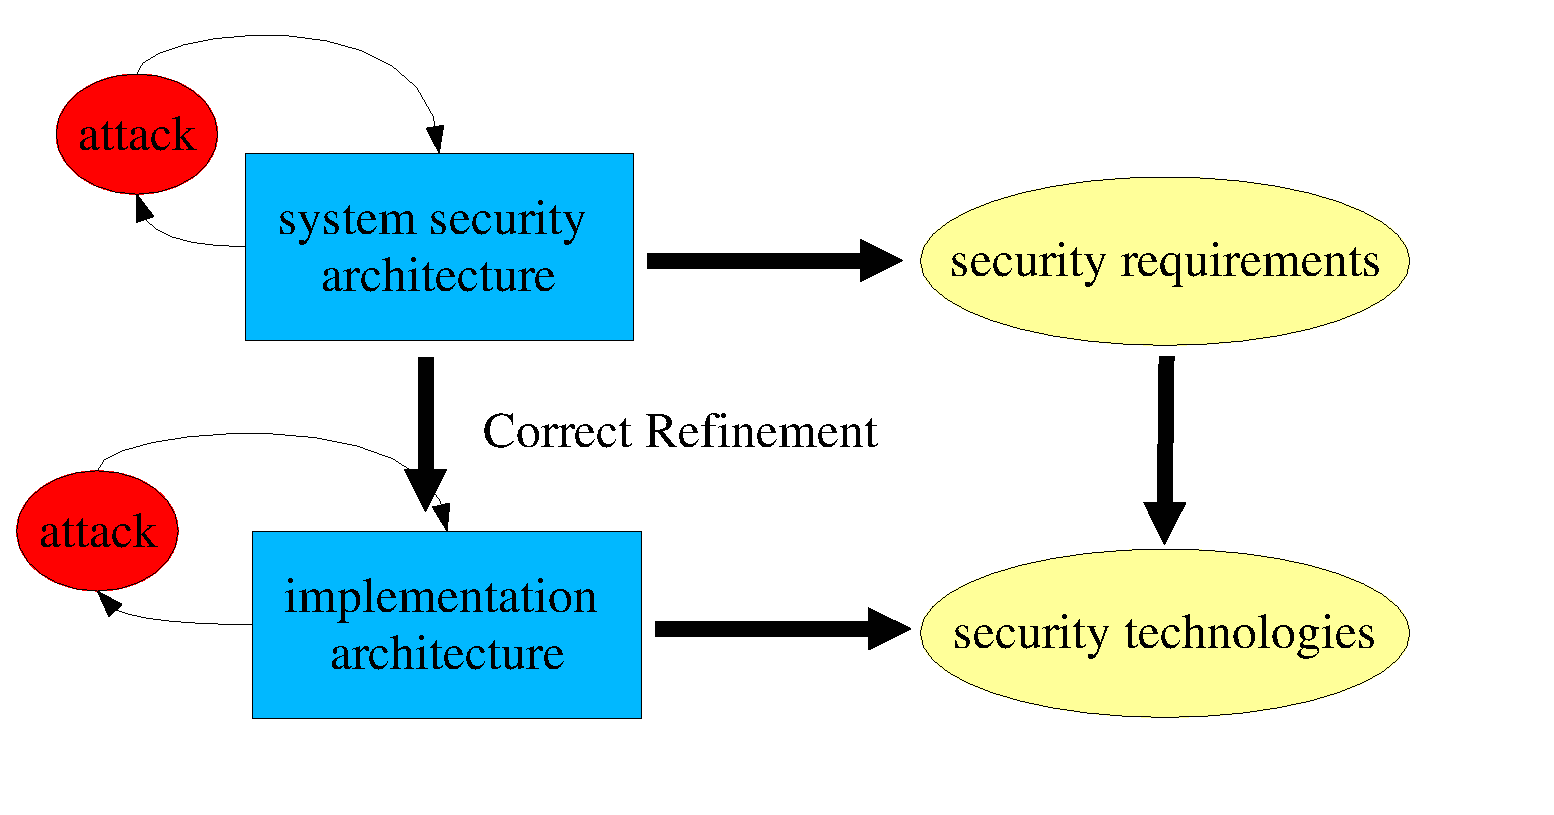
\includegraphics{pics/ref_sec1}}
    \caption{Refining Security Architectures.\label{fig:refsec1}}
\end{figure}
We have a system architecture on top, that is designed to fulfill
certain (security) requirements (a file can only be written, if a
client has an appropriate \emph{role}\index{role}, for example). This
architecture has to be mapped to an implementation architecture with
its security technologies or mechanisms (such as read/write/execute
permissions for files, for example) and security properties (a file
can't be written without write permissions, for example).  Now, we
require the security technology mapping to be correct, i.e.\ the
technologies and their properties meet indeed the security
requirements on the system architecture level.  As an
\emph{attack}\index{attack} we define a sequence of operations, that
attempt to violate a security property; if an architecture ``indeed
meets its security properties'', this means that all attacks have to
be unsuccessful.
  
In the community of formal methods, the relation between abstract and
more concrete views on a system and their semantic underpinning is
well-known under the term \emph{refinement}\index{refinement}, and
security technology mappings can be understood as a special case of
these. Various refinement notions have been proposed (As for Z,
see~\cite{woodcock.ea:using:1996} for example, as for CSP,
see~\cite{roscoe:csp:98}).  In our setting, we chose to use only a
very simple data refinement notion
following~\cite{spivey:z_notation:1992} which essentially requires
that any formula of the abstract view is implied by the formulae of
the concrete view.  Of course, following the approach taken in this
paper, we do not attempt to formally prove such a relationship.
Rather, we will check the consistency of the specifications and their
refinement relation by paper and pencil proofs. In our setting, if the
refinement relation holds, i.e.\ all operations on the concrete layer
indeed preserve the properties of the abstract layer, it can be
concluded for a \emph{correct refinement}, that attacks built by
operations of the abstract layer will not be successful, neither on
the abstract nor the concrete level.
  
Unfortunately, as shown in figure~\ref{fig:refsec2},
\emph{implementing}\index{security implementation} one security
architecture by another opens the door to \emph{new} types of attacks
on the implementation architecture, that can be completely overlooked
on the abstract level.
\begin{figure}
  \center
  \scalebox{0.5}{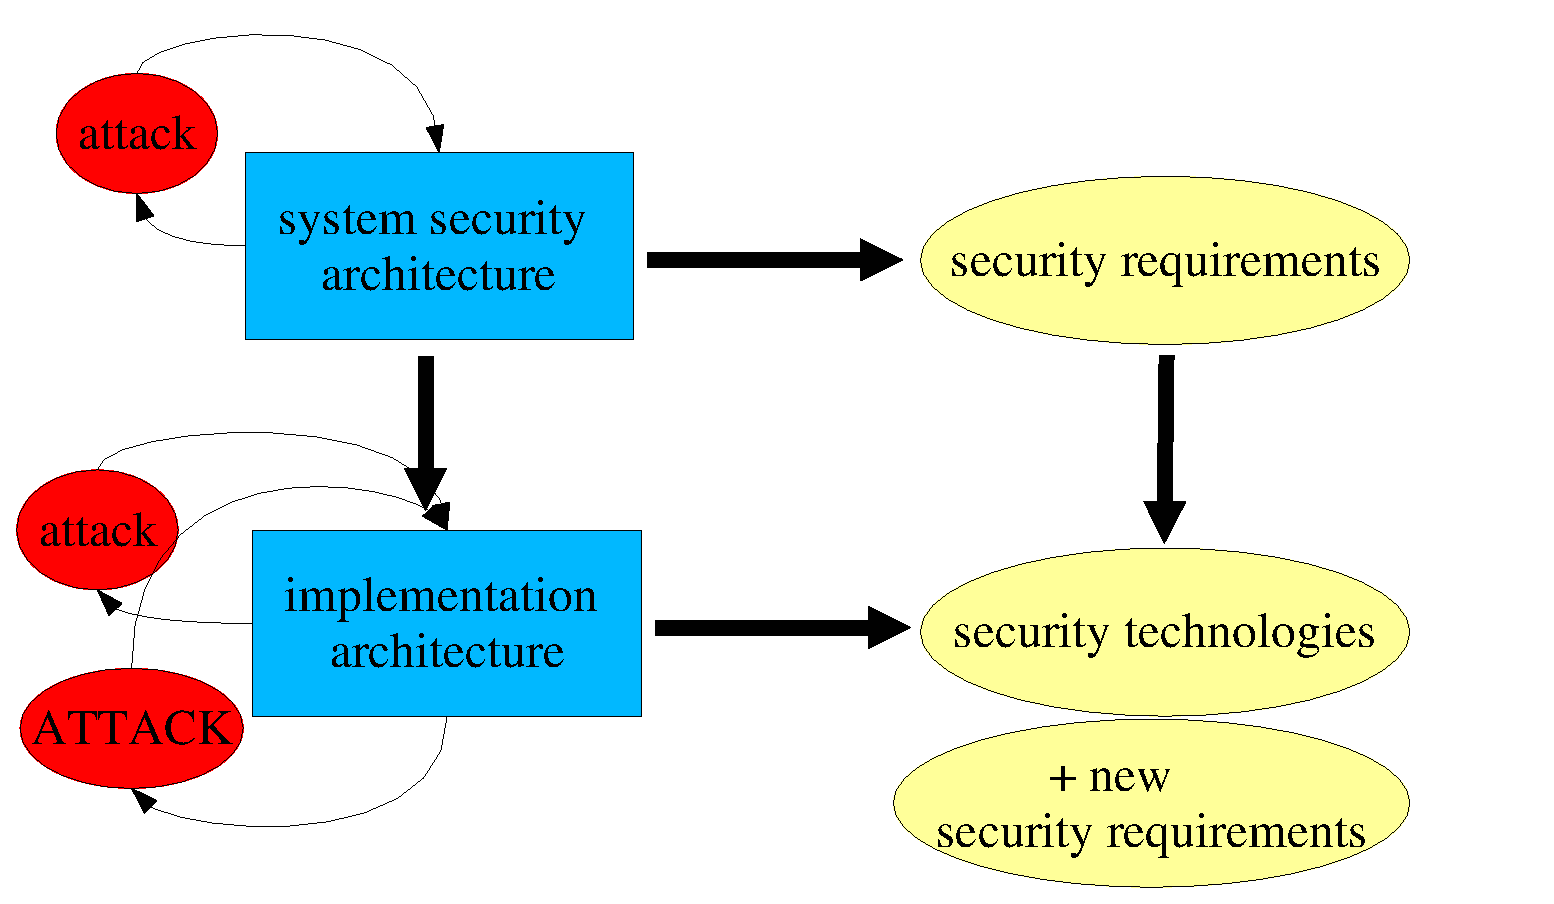
\includegraphics{pics/ref_sec2}}
  \caption{An overview of the open security architecture.\label{fig:refsec2}}
\end{figure}

These new types of attacks\index{attack} may be based on internal data
structures or internal operations of the implementation layer.  The
problem is highly relevant for our case, and, as we believe, for many
practically relevant applications and their security analysis too. In
a way, this reflects common knowledge/experience that implementing an
architecture seems to inherently ``mess up'' a security
concept\index{security concept}.  Maybe that this experience is the
deeper reason for the widespread skepticism against formal
methods\index{formal method} among implementors. However, from the
methodological viewpoint this simply means that \emph{attacks against
  the implementation}\index{attack!implementation} must simply be
taken more seriously, which implies that models of implementation
architectures are deserve more attention as before, where more
abstract models have been preferred.  But in security, more abstract
models are not necessarily better ones.

Coming back to the general refinement scenario, refining an system architecture
be a security technology mapping produces new possibilities of attacks, and
consequently new security requirements on the implementation level.

As an example, consider the instantiation of the previous scheme with our 
application scenario in~\ref{fig:refsec3}.
\begin{figure}
  \center
  \scalebox{0.5}{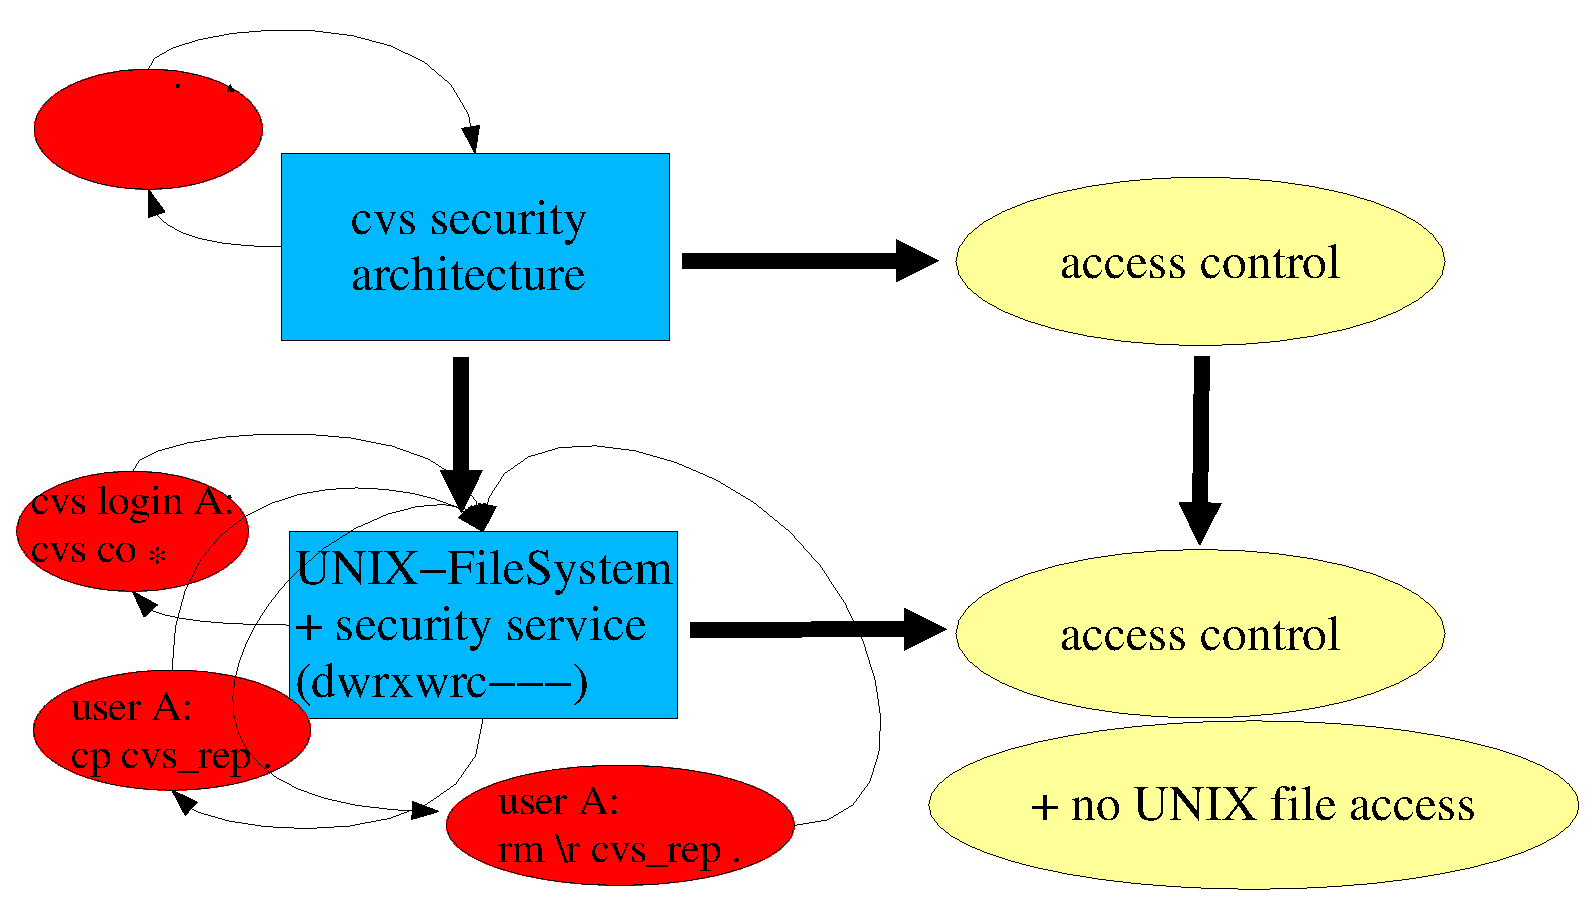
\includegraphics{pics/ref_sec3}}
  \caption{An overview of the open security architecture.\label{fig:refsec3}}
\end{figure}

Using our two-level modeling approach makes it possible to do
security analysis\index{security analysis} on both abstraction levels.
This enables also a combination-strategy of abstract and more concrete
proofs in one setting, allowing to do as much as possible on the
abstract level and concentrating the task on the concrete level to the
parts that deal with implementation specialties that may open the door
for attacks against the implementation.

\section{Performing Refinement Proofs in HOL/Z 2.0}\label{sec:holz}

HOL-Z 2.0\index{HOL-Z} is a tool chain for writing Z specifications,
type-checking them, and proving properties about them. In this
setting, we can specify our Z specifications in a type setting system,
automatically generate proof obligations, import both of them into a
theorem prover environment and use the existing proof mechanisms to
gain a higher degree of automation.  With the proof support for the
schema calculus, realistic analysis of specifications, in particular
refinement proof, in particular proofs along classical data
refinement~\cite{spivey:z_notation:1992} become feasible.

\subsection{HOL-Z: The Tool Chain for Literate Specification}
HOL-Z is now embedded in a chain of tools, that can either be integrated into
XEmacs (the way in which this document was created) or in usual
shell scripts, that allow for an easy integration of the specification process
into the general software development process.
\begin{figure}
\centering\scalebox{.5}{\input{pics/toolchain}}
\caption{A Tool Chain supporting Literate Specification\label{fig:tool-chain-supp}}
\end{figure}
The data flow in our tool chain can be described as follows: At the
beginning, a normal \LaTeX-based Z specification is created. Running
\LaTeX{} leads to the expansion of proof-obligation macros, which also
generates an Isabelle-script\index{Isabelle} that checks that the
obligations are fulfilled (to be run at a later stage).  \Zeta{} takes
over, extracts the definitions and axioms from the \LaTeX{} source
(including the generated ones) and type checks them or provides
animation for some Z schemas.  Our plug-in into \Zeta{} converts the
specification (sections, declarations, definitions, schemas, \ldots)
into SML-files that can be loaded into Isabelle.  In the theory
contexts provided by these files, usual Isabelle proof-scripts can be
developed. An integration of the process into a version management
system allows for semantically checked specifications: for example,
only when the proof obligation check scripts run successfully, new
versions of the specification document are accepted as final versions.

\subsubsection{\texttt{holz.sty} --- A Macro Package for Generating Proof Obligations}
We decided to use \LaTeX{} itself as a flexible mechanism to construct and
present proof-obligations inside the specification --- this may include
consistency conditions, refinement conditions or special safety properties
imposed by a special formal method for a certain specification architecture. Our
\LaTeX-package \verb|holz.sty| provides, among others, commands for generating
refinement conditions as described in~\cite{spivey:z_notation:1992},
where also the paradigmatical ``BirthdayBook'' is presented we use as running 
example. For $AddBirthday$ \emph{is refined by} $AddBirthday1$, we instantiate 
a macro as follows:
{\small
\begin{verbatim}
\zrefinesOp[Astate=BirthdayBook, Cstate=BirthdayBook1,
            Aop=AddBirthday, Cop=AddBirthday1,
            Args={name?: NAME; date?: DATE}, Abs=Abs]{Add}
\end{verbatim}
Here, \verb|Astate| contains the schema describing the abstract
state and \verb|Cstate| hold the schema describing the concrete state. Based
on this input, our \LaTeX-package automatically generates the following two
proof obligations:
\begin{zed}
Add_1 &==& \forall BirthdayBook;  BirthdayBook1; name?: NAME; date?: DATE @ \\
&&(\pre AddBirthday \land Abs) \implies \pre AddBirthday1\\
Add_2 &==& \forall BirthdayBook;  BirthdayBook1;  BirthdayBook1 ';name?: NAME;\\
&& date?: DATE @ (\pre AddBirthday \land Abs \land AddBirthday1)\\
&&\implies(\exists BirthdayBook ' @ Abs ' \land AddBirthday)\\ 
\end{zed}
These proof obligations are type checked using \Zeta{} and are converted to
\holz{} by our \Zeta{}-to-\holz converter. 

\subsubsection{The \Zeta-System}
\Zeta~\cite{zeta}\index{Zeta@{\Zeta}} is an open environment for the development, analysis and
animation of specifications based on Z. Specification documents are represented
by \emph{units} in the \Zeta{} system, that can be annotated with different
\emph{content} like \LaTeX{} mark-up, type-checked abstract syntax, etc. The
contents of units is computed by adaptors, which can be plugged into the system
dynamically.


\subsubsection{\Zeta-to-\holz{}Converter}
The converter consists of two parts: an adaptor that is plugged into \Zeta and
converts the type-checked abstract syntax of a unit more or less directly into an
SML file. On the SML side, this file is read and a theory context is build
inside Isabelle/HOL-Z. This involves an own type-checking and an own check of
integrity conditions of the specification and some optimizations for partial
function application in order to simplify later theorem proving.


\subsection{Proof Support for Z}
\subsubsection{Isabelle/HOL-Z revisited}
The language Z is centered around a specific structuring mechanism
called \emph{schema}\index{schema}. Semantically, schemas are just
sets of records (called \emph{bindings}\index{binding} in Z
terminology;~\cite{iso:z:2000}) of a certain type.  Z is based on
typed set theory equivalent to HOL set theory. However, a reference to
a schema can play different \emph{roles} in a specification: it can
serve as \emph{import} in the declaration list in other schemas, or as
\emph{predicate} (where all arguments are suppressed syntactically),
or as \emph{set} (see~\cite{kolyang.ea:z:96} for more details).

The approach of HOL-Z is to represent records by products in Isabelle/HOL and to
manage their layout in order to support \emph{as import}-references. This is
achieved by a parser making implicit bindings in Z expressions explicit and
generating coercions of schemas according to their role. For example, we assume
throughout this section a schema $A$ of type $[ x_1 \bindsto \tau_1, x_2
\bindsto \tau_2]$ and a schema $B$ of type $[ x_2 \bindsto \tau_2, x_3 \bindsto
\tau_3]$. Then, a schema expression $A \land B$ can be represented by
\[ \lambda (x_1,x_2,x_3)\bullet A(x_1,x_2) \land B(x_2,x_3)\;, \]
while an expression $A \cup A$ will be represented by 
$(\mathrm{asSet}~A) \cup (\mathrm{asSet}~A)$.

Thus, having ``parsed away'' the specific binding conventions of Z into standard
$\lambda$-calculus, Isabelle's proof-engine can handle Z as ordinary
HOL-formulas. There is no more ``embedding specific'' overhead such as
predicates stating the well-typedness of certain expressions, etc.

For full-automatic proofs this is fine; however, in practice, realistic case
studies require proofs with user interaction. This leads to the requirement that
intermediate lemmas can be inserted ``in the way of Z'', intermediate results
are presented ``Z-alike'' and deduction attempts to mimic the proof style
imposed by Z (cf.~\cite{woodcock.ea:using:1996}). As a prerequisite, we defined
a special abstraction operator \emph{SB} semantically equivalent to the
pair-splitting $\lambda$-abstraction from the example above, which is actually
encoded by:
\[
  \mathrm{SB}~\mbox{``$x_1$''} \leadsto x_1, \mbox{``$x_2$''} \leadsto x_2, 
  \mbox{``$x_3$''} \leadsto x_3\bullet A(x_1,x_2) \land B(x_2,x_3) 
\]
where each field-name is kept as a (semantically irrelevant) string in the
representation. Thus, while the ``real binding'' is dealt with by Isabelle's
internal $\lambda$, which is underlying $\alpha$-conversion, the
\emph{presentation} of intermediate results is done on the basis of the original
field-names used in the users specification.

\subsubsection{New Proof Support in HOL-Z 2.0}
Schemas can also be used in quantifications as part of some very Z specific
concept, the so-called \emph{schema calculus}, for which we implemented syntax 
and proof support. For
example, $\forall A \spot B$ is a schema of type $\power ([x_3 \bindsto
\tau_3])$. In HOL-Z, it is represented by:
\[ 
  \mathrm{SB}~\mbox{''$x_3$''} \leadsto x_3\bullet \forall (x_1,x_2) :
  \mathrm{asSet}~A \spot B(x_2,x_3) 
\]
This and similar quantifiers and operators allow for a very compact presentation
of typical proof-obligations occurring in refinements in Z. As example, we use 
an already slightly simplified version of $Add_1$ already described 
in~\cite[pp. 138]{spivey:z_notation:1992}. (The full proof had been omitted 
for space reasons). Instead of referring to constants representing the proof 
obligations generated by the \LaTeX-based front-end, we use the HOL-Z-parser directly:
\begin{holzverb}
zgoal thy 
"%A BirthdayBook @  %A  BirthdayBook1 @  %A  name? %:  Name @ %A date? %:  Date @ 
      (name? ~:  known /\  known = {n. ?i: #1..hwm. n=names %^ i}
       =+=> (!i : #1..hwm. name? ~=  names %^ i))";
\end{holzverb}
which opens an Isabelle proof-state.

In the literature, several calculi for the schema calculus have been presented
more or less formally (\cite{iso:z:2000,henson.ea:logic:1998}). From the
perspective of HOL-Z it is quite clear what is needed: for any construct of the
schema calculus, a special tactic must be provided that works analogously to the
usual introduction and elimination rules for standard (bounded) quantifiers and
set comprehensions. These tactics have been implemented and combined to new
tactics, for example to a tactic that ``strips-off'' all universal quantifiers
(including schema quantifiers) and implications. Thus, the HOL-Z tactic:
\begin{holzverb}
   by(stripS_tac 1);
\end{holzverb}
transforms the goal into the following proof state:
\begin{holzverb}
1. !!birthday known dates hwm names name? date? i.
    [| BirthdayBook (birthday, known); BirthdayBook1 (dates, hwm, names);
       name? : Name; date? : Date;
       name? ~:  known /\  known = {n. ?i: #1..hwm. n=names %^ i};
       i : ( #1 .. hwm) |] ==> name? ~=  names %^ i
\end{holzverb}
Note that the quite substantial reconstruction of the underlying binding still
leads to a proof state that is similar in style and presentation
to~\cite{woodcock.ea:using:1996}.

Besides the ``schema calculus'', Z comes with a large library of set operators
specifying relations, functions as relations, sequences and bags; this library
--- called the \emph{Mathematical Toolkit} of Z --- differs in style
substantially from the Isabelle/HOL library, albeit based on the same
foundations. For HOL-Z 2.0, we improved this library substantially and added
many derived rules that make a higher degree of automatic reasoning by
Isabelle's standard proof procedures possible. For example, the goal above is
simply ``blown away'' by:
\begin{holzverb}
   auto();
\end{holzverb}
which finishes the proof.
%%% Local Variables:
%%% TeX-master: "arch"
%%% fill-column:80
%%% x-symbol-8bits:nil
%%% End:

s\rcsInfo $Id: sys-arch.tex,v 1.37 2004/01/29 10:36:23 hiss Exp $

\chapter{A Formal Model of the System Security Architecture}\label{cha:sys-arch}

In this section, we will describe the more abstract view of our system. In order
to avoid unnecessary complexity, we will reduce our architecture to exactly one
client communicating with the server.  This is realistic since the CVS server
processes all requests sequentially and different clients could be modeled by
one client logging in and out with different user IDs and roles.  We will model
the state of a client and the state of the CVS repository and the operations the
combined system may perform.  These operations include read and write access of
clients to the repository and allow for a fairly compact description of the
access control policy the CVS-Server may enforce.

This access control policy is well known as \emph{role-based access
  control}\index{RBAC}\index{role-based access control}. In
\cite{sandhu.ea:role-based:1996}, a formal framework of role-based
access control is described that introduces the \rbac-model for role
hierarchies that is closely related to the security policy enforced by
our system architecture.  However, we differ from \rbac{} in a number of
minor issues in order to get a model that can be refined to the
implementation architecture.  For instance, we will \emph{not} model
\emph{sessions} of \rbac directly.  Moreover, since we assume a
one-to-one correspondence between roles and permissions (i.e.\ the
\emph{permission assignment $(PA)$}\index{permission assignment} is a
bijective function), we directly define the role hierarchy $(RH)$ on
permissions, which is more convenient for technical reasons.  Further,
since the administrator is part of the model (the authorization for a
user may thus be dynamically withdrawn), the pair consisting of a
\emph{user ID}\index{user ID} and its authentication (a
\emph{password}\index{password}) representing a \emph{permission} has
to be kept in the user state and can not be evaluated to a permission
for the whole session during login-time; rather, for any access to the
repository, the system checks (as the real CVS-Server) if the pair
still represents a valid permission at access-time.

Besides the access operations, we introduce a
\emph{login}\index{login} operation that marks the entry of a session
(if we neglect the dynamic aspect of authentication).  During the
login operation, a user authenticates for a role; this operation
either results in a change of the permissions of the client state
corresponding to that user or in a failure.


\section{Fundamental Entities of the Model}\label{sec:basics}

%%macro \zcomment 1

\zsection{Basics}\vspace{1ex}\noindent

Common to both architectural models is an adopted \rbac-model.  Therefore, we
introduce basic data types for users, permissions (one particularity of our
model is the isomorphism of roles and permissions), and passwords for
authenticating.
\begin{zed}
  [ Cvs\_Uid, Cvs\_Perm, Cvs\_Passwd ]
\end{zed}

The role hierarchy\index{role!hierarchy} is captured by a reflexive,
transitive relation with the administrative permissions ($cvs\_admin$)
as greatest and the permissions for public access ($cvs\_public$) as
least element.  Since roles and permissions are isomorphic in our
model, for convenience, we define the order directly on permissions.
\begin{doc}{4}
  \begin{axdef}
    cvs\_admin, cvs\_public : Cvs\_Perm \\
    cvs\_perm\_order        : Cvs\_Perm \rel Cvs\_Perm \\
    \where
    cvs\_perm\_order = cvs\_perm\_order \star \\
    \forall x: Cvs\_Perm @ (x,cvs\_admin) \in cvs\_perm\_order \\
    \forall x: Cvs\_Perm @ (cvs\_public,x) \in cvs\_perm\_order \\
    \forall x: Cvs\_Perm @ (x \neq cvs\_admin)\implies (cvs\_admin,x) \notin cvs\_perm\_order \\
    \forall x: Cvs\_Perm @ (x \neq cvs\_public)\implies (x, cvs\_public) \notin cvs\_perm\_order \\
    \forall x: Cvs\_Perm @ \exists y: Cvs\_Perm @ (x,y) \in cvs\_perm\_order\\
  \end{axdef}
\end{doc}

For authentication\index{authentication} and
authorization\index{authorization} of the client upon him accessing
the repository or for logging in, we need a fixed preconceived table
that associates permissions to an ID, a client has authenticated for
with his password.  Additionally, we define a table that associates to
CVS user IDs the corresponding passwords.  The client state of our
model will manage such a table.
\begin{zed}
  AUTH\_TAB == Cvs\_Uid \cross Cvs\_Passwd \pfun Cvs\_Perm \\
  PASSWD\_TAB == Cvs\_Uid \rel Cvs\_Passwd \\
\end{zed}


\section{The State of the System Architecture}

\zsection[Basics]{AbstractState}\vspace{1ex}\noindent

As a basis to define the system state and its operations in the Z-sections
\texttt{AbsState} and \texttt{AbsOperations} we have to define Z data types that
represent files (a mapping from names to data), and data types for modeling
access control properties, e.g., necessary permissions to access data.
\begin{zed}
  [Abs\_Name, Abs\_Data] \\
  ABS\_DATATAB == Abs\_Name \pfun Abs\_Data \\
  ABS\_UIDTAB == Abs\_Name \pfun Cvs\_Uid \\
  ABS\_PERMTAB == Abs\_Name \pfun Cvs\_Perm \\
\end{zed}
CVS server store their authentication table inside the repository --- thus, the
table can be accessed and modified using the operations of CVS\@. We will
capture this fact in our model; as a prerequisite, we define a name
$abs\_cvsauth$ to which data is associated, that is isomorphic to an
authentication table. This isomorphism is established by a pair of functions ---
that can be viewed as \emph{parser} and \emph{pretty\_printer} --- and the usual
axioms.
\begin{axdef}
  abs\_cvsauth: Abs\_Name \\
  abs\_auth\_of: Abs\_Data \pfun AUTH\_TAB \\
  abs\_data\_of: AUTH\_TAB \fun Abs\_Data \\
  authtab   : ABS\_DATATAB \pfun AUTH\_TAB \\
  \where
  \ran(abs\_data\_of) \subseteq \dom(abs\_auth\_of) \\
  \forall x : \dom abs\_auth\_of @ abs\_data\_of(abs\_auth\_of~x) = x \\
  \forall x : AUTH\_TAB @ abs\_auth\_of(abs\_data\_of~x) = x \\
  \forall r : ABS\_DATATAB @   abs\_cvsauth \in \dom(r) \implies \\
  \t2 authtab(r) = abs\_auth\_of(r~abs\_cvsauth) \\
\end{axdef}

A vital predicate for the access control is the predicate $has\_access$.  It
checks according to the underlying data-structures of the server, if the user
has for a particular $Cvs\_Uid$ (i.e.\ a ``role'') and a particular $file$ access
in the repository. This requires:
\begin{enumerate}
\item that role and actual password are defined in the authentification
      table in the repository,
\item and that the resulting permission from the authentification
      is sufficient with respect to the permission ordering.
\end{enumerate}
Formally, this predicate looks as follows:
%%prerel has\_access
\begin{axdef}
  has\_access \_ :\power(ABS\_PERMTAB\cross ABS\_DATATAB\cross PASSWD\_TAB\cross Abs\_Name\cross Cvs\_Uid)
  \where
  \forall rep\_pt : ABS\_PERMTAB; rep:ABS\_DATATAB; pwtb : PASSWD\_TAB; \\
    \t1 file:Abs\_Name; role: Cvs\_Uid @ \\
    \t2 has\_access(rep\_pt,rep,pwtb,file,role)  \iff \\
    \t3 (role, pwtb(role)) \in \dom(authtab~rep) \\
    \t3 \land (rep\_pt(file),authtab(rep)(role, pwtb(role)))\in cvs\_perm\_order
\end{axdef}


Note that the parser $abs\_auth\_of$ is a partial function; this models the fact
that not all file contents do actually represent input that can be interpreted.
Moreover, we did not make any assumptions on authentication tables $AUTH\_TAB$;
for example, a requirement like ``there is someone that can authenticate as
$cvs\_admin$'' (i.e.  $ cvs\_admin \in \dom at$ where $at : AUTH\_TAB$) would be
helpful but is omitted since the real CVS-Server does not make this assumption.
This has far reaching consequences; in particular, it is possible to bring the
CVS server into a state where all operations block since all authentications
fail, which resembles a \emph{denial of service
  attack}\index{attack!denial of service} at the \posix-layer.

In the remainder of this section, we define the states of the client and the
server component.  To motivate the details of our specification, we present an
excerpt from the informal description of the CVS \cvscmd{login} command:
\begin{quote}
  \emph{Contacts a CVS server and confirms authentication information for a
    particular repository. This command does not affect either the working copy
    or the repository; it just confirms a password with a repository and stores
    the password for later use in the .cvspass file in your home directory.
    Future commands accessing the same repository with the same username will
    not require you to rerun login, because the client-side CVS will just
    consult the .cvspass file for the password.}~\cite{fogel:cvs:1999}
\end{quote}
The state of the client ($ClientState$) captures the concept of a working copy
in the variable $wc$, a set of files, and also introduces $wc\_uidtab$ which is
used to record for each file in the working copy the user ID that was used to
access this file in the repository.  The above mentioned file ``.cvspass'' is
modeled by $abs\_passwd$ which is a set of pairs of user IDs and passwords the
client has logged in with.  In addition, we introduce a set of focused files
($wfiles$) which will be the implicit arguments for most CVS operations.
\begin{doc}{ClientState}
  \begin{schema}{ClientState}
    wfiles: \power Abs\_Name \\
    wc: ABS\_DATATAB \\
    wc\_uidtab: ABS\_UIDTAB \\
    abs\_passwd: PASSWD\_TAB \\
  \end{schema}
\end{doc}
It is straightforward to motivate the state $RepositoryState$ of the server
component: The central concept of CVS is the repository, a set of files, which
is defined as $rep$.  Since the access to each file is checked individually, we
also define $rep\_permtab$, a table that associates the required access
permissions to each file.

As mentioned above, CVS-Server stores the authentication data inside the
repository --- thus it can be accessed and modified with CVS operations.  To
model this, we introduce a name $abs\_cvsauth$ and auxiliary functions.  In the
server state, we now require that $abs\_cvsauth$ is a file in the repository,
and that only the CVS administrator has sufficient permissions to access the
authentication data, i.e.\ we set the necessary permission to the greatest
element $cvs\_admin$ of our permission/role hierarchy.
\begin{doc}{RepositoryState}
  \begin{schema}{RepositoryState}
    rep: ABS\_DATATAB \\  
    rep\_permtab: ABS\_PERMTAB \\
    \where
    abs\_cvsauth \in \dom rep \\
    \dom rep = \dom rep\_permtab \\
    rep\_permtab(abs\_cvsauth) = cvs\_admin \\
    rep(abs\_cvsauth) \in \dom abs\_auth\_of \\ 
  \end{schema}
\end{doc}


\section{The Operations of the System Architecture}

\zsection[AbstractState]{AbsOperations}\vspace{1ex}\noindent

Now we define the operations of the system that model combined state transitions
of the client and the repository.  We begin with the \cvscmd{login} operation of
our CVS-Server system architecture.  Logging in marks the begin of a session, in
which the client authenticates for permissions that control his access to the
repository.  The operation \cvscmd{cd} sets the focused files ($wfiles$) for the
following operations.
\begin{zedgroup}
  \begin{doc}{absops_login}
    \begin{schema}{abs\_login}
      \Delta ClientState \\
      \Xi RepositoryState \\
      passwd?: Cvs\_Passwd \\
      uid?: Cvs\_Uid \\
      \where
      (uid?,passwd?) \in \dom (authtab~rep) \\
      abs\_passwd' = abs\_passwd \\
      \t1 \oplus \{ uid? \mapsto passwd? \} \\
      wc' = wc \\
      wc\_uidtab' = wc\_uidtab \\
      wfiles' = wfiles \\
    \end{schema}
  \end{doc}
  \begin{doc}{absops_cd}
    \begin{schema}{abs\_cd}
      \Delta ClientState \\
      \Xi RepositoryState \\
      wfiles?: \power Abs\_Name \\
      \where
      wfiles' = wfiles? \\
      wc' = wc \\
      wc\_uidtab' = wc\_uidtab \\
      abs\_passwd' = abs\_passwd \\
    \end{schema}
  \end{doc}
\end{zedgroup}

The next three operations allow for a synchronization of the working copy with
the operations. Recall that our model deliberately neglects all aspects related
to version control and merging of files; our model focuses on the security
aspects of the CVS-Server.

The \cvscmd{add} operation mirrors the fact that the user has created new
content (new filenames as well as new associated data). The operation adds this
new data to the local working copy and makes sure that the new names are
actually new in the repository.
\begin{doc}{absops_add}
  \begin{schema}{abs\_add}
    \Delta ClientState \\
    \Xi RepositoryState \\
    newfiles?: ABS\_DATATAB \\
    \where
    \dom newfiles? \cap \dom rep = \emptyset \\
    wc' = wc \oplus newfiles?  \\
    wc\_uidtab'= wc\_uidtab \oplus \{ n : \dom newfiles? | n \notin \dom wc\_uidtab \\
    \t2  \land (\exists id : \dom abs\_passwd @ \\
    \t3 (id, (abs\_passwd~id)) \in \dom (authtab~rep)) @\\
    \t2 n \mapsto (\mu id:
    \dom abs\_passwd | (id, (abs\_passwd~id)) \in \dom (authtab~rep)) \} \\
    wfiles' = wfiles \\
    abs\_passwd' = abs\_passwd \\
  \end{schema}
\end{doc} 
The \cvscmd{commit} and \cvscmd{checkin} operations usually take a set if files
as arguments (here denoted by $files?$).  However, if no arguments are provided
then these operations use the set of currently focused files ($wfiles$) as
implicit arguments.  This is modeled by restricting $files?$ by 
$wfiles$\footnote{Note that in order to operate on the
complete set of focused files, $files?$ must be equal to $wfiles$.}.

In our model the \cvscmd{commit} (or \cvscmd{checkin}) operation assumes that 
for all focused files (restricted by the input parameter), the user actually has access
to these files in the repository, i.e.\ his actual permission is larger than the
required one in the repository\footnote{We slightly oversimplified the
  situation for the sake of the presentation: the real implementation actually
  filters out the non-accessible files, while in our model, the operation
  blocks.}. For these files, the content of the working copy is transferred to
the repository. Note the use of $wc'$ here to mirror the fact that the data in
the working copy may have changed non-deterministically by user interaction and
merge operations which are excluded from our model.
\enlargethispage{\baselineskip}
\begin{doc}{absops_ci}
  \begin{schema}{abs\_ci}
    \Xi ClientState \\
    \Delta RepositoryState  \\
    files?: \power Abs\_Name \\
    \where
    (wfiles \cap files?) \subseteq \dom wc \\

    rep' = rep \oplus (\{ n: wfiles \cap files? | n \notin \dom rep \land n \in
    \dom wc\_uidtab \\
    \t1 \land (wc\_uidtab(n), abs\_passwd(wc\_uidtab~n)) \in
    \dom(authtab(rep))\} \dres wc) \\  
    \t2 \oplus (\{n : wfiles \cap files? | n \in \dom rep \land n \in \dom
    wc\_uidtab \\
    \t2 \land has\_access(rep\_permtab,rep,abs\_passwd,n,wc\_uidtab(n))\}
    \dres wc) \\

    rep\_permtab' = rep\_permtab \oplus \{ n: wfiles \cap files? |  n \notin
    \dom rep \land n \in \dom wc\_uidtab \\
    \t1 \land (wc\_uidtab(n), abs\_passwd(wc\_uidtab~n)) \in \dom(authtab~rep) @
    \\
    \t2 n \mapsto authtab(rep)(wc\_uidtab(n), abs\_passwd(wc\_uidtab~n)) \} \\

  \end{schema}
\end{doc}

The \cvscmd{update} operation updates every file in the working copy by the
corresponding file in the repository if the client has sufficient permissions to
access the file in the repository, i.e., is in a senior enough role. This
operation does not block if the client does not have sufficient permissions, but
silently ignores those files.  Additionally, this operation also updates the
permission table in the working copy.  If an accessible file does not exist in
the working copy $wc$ of the client, then $abs\_up$ simply inflates it from the
repository. Otherwise, CVS \cvscmd{update} originally distinguishes between four cases. The
working copy is \ldots
\begin{itemize}
  \item up-to-date and not locally modified. There is no action.
  \item up-to-date and locally modified. The message \glqq locally
    modified\grqq{} is displayed.
  \item outdated but not locally modified. The old version is replaced by the
    new one.
  \item both outdated and locally modified. An RCS~\cite{tichy85rcs}\index{RCS} merge
    operation (a 3-way-merge) is used to combine the working copy, the version
    in the repository and the latest ancestor which they have in common. This is
    the version of the file in the repository with the revisionnumber of the
    corresponding file of the working copy.
\end{itemize}

In our model we simplify this procedure using a non-deterministic merge
operation which implicitly handles all four cases.

\begin{doc}{3}
  \begin{axdef}
    merge : (Abs\_Data \cross Abs\_Data) \fun Abs\_Data \\
    \where
    \forall x : Abs\_Data @ merge(x,x) = x \\
  \end{axdef}
\end{doc} 

\begin{doc}{absops_up}
  \begin{schema}{abs\_up}
    \Delta ClientState \\
    \Xi RepositoryState  \\
    files?: \power Abs\_Name \\
    \where 
%wc' = wc \oplus (\{ n: wfiles \cap files? | n \in \dom rep \land n \in \dom
%    wc\_uidtab \\
%    \t1 \land (wc\_uidtab(n), abs\_passwd(wc\_uidtab~n)) \in \dom(authtab~rep) \\
%    \t1 \land (rep\_permtab(n),authtab(rep)(wc\_uidtab(n), \\
%    \t2 abs\_passwd(wc\_uidtab~n)))\in cvs\_perm\_order\} \dres rep) \\
wc' = wc \oplus (\{ n: wfiles \cap files? | n \notin \dom wc \land n \in \dom rep \land n \in \dom
    wc\_uidtab' \\
    \t1 \land has\_access(rep\_permtab,rep,abs\_passwd,n,wc\_uidtab'(n))\} \dres rep) \\    
    \oplus \{ n: wfiles \cap files? | n \in \dom wc \land n \in \dom rep \land n \in \dom
    wc\_uidtab \\
    \t1 \land has\_access(rep\_permtab,rep,abs\_passwd,n,wc\_uidtab(n)) @ n \mapsto (merge(rep(n), wc(n)))\}\\

    wc\_uidtab' = wc\_uidtab \oplus \{ n: wfiles \cap files? |  n \in \dom rep \\
    \t1 \land n \notin \dom wc\_uidtab \land (\exists id : \dom abs\_passwd @ \\
    \t2 has\_access(rep\_permtab,rep,abs\_passwd,n,id)) @\\
    \t2 n \mapsto (\mu id: \dom abs\_passwd | has\_access(rep\_permtab,rep,abs\_passwd,n,id)) \} \\

    abs\_passwd' = abs\_passwd \land wfiles' = wfiles \\
  \end{schema}
\end{doc}

In addition to these abstract models of the CVS operations we provide a modify operation which explicitly models interactions of users with their files via modifying the files of the working copy of the client state.

\begin{doc}{absops_modify}
  \begin{schema}{modify}
    \Delta ClientState \\
    \Xi RepositoryState  \\
    filename? : Abs\_Name \\
    newData? : Abs\_Data \\
    \where 
    filename? \in \dom wc\\
    wc' = wc \oplus\{ filename? \mapsto merge(wc~filename?, newData?)\} \\
    wfiles' = wfiles \\
    wc\_uidtab' = wc\_uidtab \\
    abs\_passwd' = abs\_passwd \\
  \end{schema}
\end{doc}

%%% Local Variables:
%%% TeX-master: "arch"
%%% fill-column:80
%%% x-symbol-8bits:nil
%%% End:


\rcsInfo $Id: impl-arch.tex,v 1.50 2003/12/04 15:03:06 brucker Exp $

\chapter{A Formal Model of the Implementation Security Architecture}\label{cha:form-model-impl} 

\section{The POSIX Security Architecture}\label{sec:posix-secur-arch}

We implement our role-based access control model by embedding it into the
Discretionary Access Control (DAC\index{DAC}\index{Discretionary
  Access Control@see{DAC}}) as provided by the \unix{} operating system
and its hierarchic filesystem layer. This specific DAC implementation was first
described in POSIX.1\index{POSIX} and adopted by the ``Single UNIX Specification Version
2'' (Unix98)~\cite{open:unix:1997}, a
standard all modern \unix variants follow. This DAC is also described in the
common successor of these two documents, which is ``The Single UNIX
Specification Version 3''~\cite{open:unix:2002}\index{Single UNIX Specification}; referenced in the following as
\susv.

In this chapter, we define a formal model of this filesystem specification, and
use it as a basis for specifying the implementations of the CVS commands.  

\subsection{Prelude}

\zsection{Prelude}\vspace{1ex}\noindent

The following structure is a foundational part of our specification.
Essentially, type sums are introduced, that are not part of the standard. Type
sums can simulate enumerations in Z free type definitions on the fly. In the
following, we define type sums via a generic schema in Z\footnote{While generic
  schemes are not accepted by HOL-Z 2.0, type sums are compiled via another
  mechanism and are therefore exceptionally accepted.}.

$Prelude\_SUM$ just serves as a tag of the type for the translation.
\begin{zed}
  [Prelude\_SUM]
\end{zed}
\zfunction{30 (\_ \pplus \_)}
\begin{gendef}[X,Y]
  \_ \pplus \_ : X \cross Y \fun \power (Prelude\_SUM \cross X \cross Y) 
\end{gendef}
\begin{gendef}[X,Y]
  Inl   : X \fun (X \pplus Y) \\
  Inr   : Y \fun (X \pplus Y) \\ 
\end{gendef}
The definition of injection functions or recursors is omitted; the declarations
above serve as pure type interface. A semantic definition of these constructs is
straightforward, however.


\subsection{The Basic Data Structures}

\zsection[Prelude,Basics]{FileSystem}\vspace{1ex}\noindent

In the following, we declare basic abstract sorts for \unix user IDs,
group IDs, data (file contents; left abstract in this
model)\index{ID}\index{ID!user}\index{ID!group} and filenames. The
file hierarchy\index{file hierarchy} is left implicit in our model; it will be essentially
captured by some kind of ``prefix-closedness'' on legal paths\index{path} in the
filesystem.  Additionally, we define an enumeration $Unit$ which will
be used to distinguish directories\index{directory} from regular files\index{file!regular}.
\begin{zed}
  [ Uid, Gid, Data, Name ] \\
  Path == \seq Name \\
  Unit ::= Nil \\
\end{zed}

In our model, we assume a static table \emph{groups} that assigns a set of
groups to each user. The axiomatic definition below also states the existence
of a special user ID $root$ which models the system administrator (usually
called \textit{root}). In principle, all security properties can only hold for
all users except $root$, because root is allowed to do (almost) everything in a
\unix system.
\begin{doc}{root_groups}
  \begin{axdef}
    groups: Uid \fun \power Gid \\
    root: Uid \\
  \end{axdef}
\end{doc}

The function $cutPath$ removes a given prefix from a path.
\begin{axdef}
  cutPath: (Path \cross Path) \pfun Path \\
  \where
  \forall a,b,c: Path @ cutPath(a,b) = c \iff  a = b \cat c \\
\end{axdef}

Now we introduce the set of permissions\index{permission}, including the ``set-uid bits'': Within
\unix{} every file belongs to a unique pair of owner (user) and group.
Logically \emph{file access}\index{file access} is divided into three classes:
\begin{enumerate}
\item Access by the \emph{user} (owner\index{owner}\index{file!owner}) of the file,
\item access by a member of the \emph{group}\index{group}\index{file!group} the file is owned by, or
\item access by any \emph{other}\index{other} user (world).
\end{enumerate}
Further, the standard \unix{} DAC\index{DAC} distinguishes between access for reading
(\unixcmd{r}), writing (\unixcmd{w}), and executing (\unixcmd{x}).\footnote{For
  directories, this can be interpreted as access for searching in the directory
  (\unixcmd{r}), creating new files or subdirectories (\unixcmd{w}) and entering
  (\unixcmd{x}) the directory.}  The execution model\index{execution model} of \unix{} further
introduces the set-id\index{set-id} (for owner and group) and the
sticky bit\index{sticky bit}. Our model uses
only the set-gid\index{set-gid} (set-id for groups) facility on directories, which affects the
default group of newly created files within that directory. We exclude the
set-id bit, and the sticky bits, whose semantics has changed over time, and
therefore can possibly have different semantics within the different
\unix-implementations (a detailed discussion of the different implementations is
for example given in~\cite{frisch:administration:1995}).  Apart from that, the
sticky bits are irrelevant for our problem and are not used by our
implementation either.
\begin{zed}
Perm  &::= &    ru | wu | xu \\
      &    &  | rg | wg | xg \\
      &    &  | ro | wo | xo \\
      &    &  | sg \\
\end{zed}

The filesystem consists of files which are represented by mapping the
file content to each path, which is either $Data$ for regular
files\index{file!regular} or $Unit$ for directories\footnote{We do not
  consider \emph{special files}\index{file!special}, like devices,
  named pipes or process files.}\index{file!directory}, and of file
attributes (assigning to each file or directory the
permissions\footnote{Often the terms
  \emph{attributes}\index{attribute} and
  \emph{permissions}\index{permission} are used interchangeably.}, the
user ID of the owner and the group it belongs to). In the following,
if we speak only of \emph{files} we mean a regular file or a
directory.  Note that our concept of file attributes may be extended
easily by adding new components to its records.
\begin{zed}
  FILESYS\_TAB == Path \pfun (Data \pplus Unit) \\
  FILEATTRIBUTES == [ perm: \power Perm; uid: Uid; gid: Gid ] \\
  FILEATTR\_TAB == Path \pfun FILEATTRIBUTES \\
\end{zed}

For testing if a directory contains a specific file we provide the function
$\isin$.  Further we provide functions that test for regular files ($\isfilein$)
and for directories ($\isdirin$).
% \zfunction{30 (\_ \isdirin \_)}
%\begin{verbatim}
%%inrel \isdirin
%%inrel \isfilein
%%inrel \isin
%\end{verbatim}
\begin{axdef}
  \_ \isin \_     : Path  \rel (Path \pfun (Data \pplus Unit))  \\
  \_ \isdirin \_  : Path  \rel (Path \pfun (Data \pplus Unit))  \\
  \_ \isfilein \_ : Path  \rel (Path \pfun (Data \pplus Unit))  \\
  \where
  \forall fs: (Path \pfun (Data \pplus Unit)); f: Path @ \\
  \t1 (f \isin fs) \iff f \in \dom fs \\

  \forall fs: (Path \pfun (Data \pplus Unit)); d: Path @ \\
  \t1 (d \isdirin fs) \iff (d \isin fs) \land (\exists u: Unit @ fs(d) = Inr(u))
  \\

  \forall fs: (Path \pfun (Data \pplus Unit)); f: Path @ \\
  \t1 (f \isfilein fs) \iff (f \isin fs) \land \lnot (f \isdirin fs) \\
\end{axdef}
  

\subsection{The Filesystem State}

At this point we are ready to model the filesystem state, which mainly describes
the set of existing files and their attributes.  The filesystem has to obey the
following two invariants:
\begin{enumerate}
\item All defined paths must be ``prefix-closed'', i.e.\ all prefix paths must
  be defined in the filesystem (thus constituting a tree) and point to
  directories, and
\item file attributes must be defined for every file in the filesystem.
\end{enumerate}
\begin{doc}{FileSystem}
  \begin{schema}{FileSystem}
    files: FILESYS\_TAB \\
    attributes: FILEATTR\_TAB \\
    \where
     \forall p: \dom files @ (p = \langle \rangle) \lor (front(p) \isdirin
     files) \\ 
    \dom files = \dom attributes \\
  \end{schema}
\end{doc}

%%% stolen axioms...
%%\begin{axdef}
%%  files\_has\_root: \nat \\
%%  \where
%%  \forall FileSystem @ \dom files \neq \emptyset \implies \langle \rangle \in
%%  \dom files \\
%%\end{axdef}

First we introduce a function $has\_attrib$, which decides whether the
attributes (read, write and execute) of a file are set with respect to a
specific user (and the groups he is a member of). Within this function, a
nitpicking detail of the \susv{} access model is formalized, namely (local) file
access is strictly tested in the following order and testing ends whenever a
test for access fails\index{file!access}:
\begin{itemize}
\item If the user owns the file, he can only access the file if the access
  attributes for users ($\{ru,wu,xu\}$) grant access.
\item If the user is a member of the group owning the file, he can access the
  file if the access attributes for the group ($\{rg, wg, xg\}$) grant access.
\item In all other cases the access attributes for others ($\{ro,wo,xo\}$) are
  checked.
\end{itemize}
This testing strategy leads to the strict precedence of owner permissions over
the group or other permissions and to the following detail, which seems to be a
little awkward at first sight: Assume the user $u$ who is a member of the group
$g$ tries to read a file, owned by him, with permissions $\lblot
perm==\{rg,ro\},uid==u,gid==g \rblot$. Is the user $u$ allowed to read the file?
Astonishingly, this is not the case because the rights specified for the user
$u$ (who is also the owner of the file) precede the rights given for the group
or others.  Therefore this file can only be read by all users not member of
group $g$ and all members of group $g$ except the user $u$.  Using the same
``trick'' it is possible to specify permissions for a file that is readable for
all users except the members of one specific group.

Based on $has\_attrib$ we introduce $has\_r\_attrib$, $has\_w\_attrib$ and
$has\_x\_attrib$ for testing the read, write and execute attributes.
%%prerel has\_attrib
%%prerel has\_r\_attrib
%%prerel has\_w\_attrib
%%prerel has\_x\_attrib
\begin{doc}{3}
\begin{axdef}
  has\_attrib \_ : \power(Uid\cross Path\cross FILEATTR\_TAB\cross Perm\cross Perm\cross Perm)\\ 
  \where
  \forall uid : Uid; fa : FILEATTR\_TAB; pu,pg,po:Perm @ \forall p : \dom(fa) @\\
  \t1 has\_attrib(uid,p,fa,pu,pg,po) \iff \\
  \t2 ((uid = root) \lor
  \t2  (\forall m: \power Perm; diruid : Uid; dirgid : Gid |\\
  \t3 \lblot perm==m,uid==diruid,gid==dirgid\rblot =fa(p) @\\
  \t4 (diruid = uid \land pu \in m)  \lor                       \\
  \t4 (diruid \neq uid \land dirgid \in groups(uid) \land pg \in m) \lor \\
  \t4 (diruid \neq uid \land dirgid \notin groups(uid) \land po \in m))) \\
\end{axdef}
\begin{axdef}
  has\_r\_attrib \_ : \power (Uid \cross Path \cross FILEATTR\_TAB) \\
  has\_w\_attrib \_ : \power (Uid \cross Path \cross FILEATTR\_TAB) \\
  has\_x\_attrib \_ : \power (Uid \cross Path \cross FILEATTR\_TAB) \\
  \where

  \forall uid : Uid; p : Path; fa : FILEATTR\_TAB @ \\
  \t1 has\_r\_attrib(uid,p,fa) \iff has\_attrib(uid,p,fa,ru,rg,ro) \\
  
  \forall uid : Uid; p : Path; fa : FILEATTR\_TAB @ \\
  \t1 has\_w\_attrib(uid,p,fa) \iff has\_attrib(uid,p,fa,wu,wg,wo) \\
  
  \forall uid : Uid; p : Path; fa : FILEATTR\_TAB @ \\
  \t1 has\_x\_attrib(uid,p,fa) \iff has\_attrib(uid,p,fa,xu,xg,xo) \\
\end{axdef}
\end{doc}

For accessing a specific file described by an absolute path name, it is not
sufficient to test the file attributes\index{file!access}.  Access to the directory containing that
file also has to be granted. In particular, we need to be able to enter each
directory (the execution bit has to be set) along the path. Here it makes no
difference if the ``enter'' access is granted based on user, group or other
permissions.  This is described in the functions $has\_w\_access$ and
$has\_r\_access$ for testing if a user can write or read a file.
%%prerel has\_w\_access
%%prerel has\_r\_access
%%prerel has\_x\_access
\begin{doc}{3}
  \begin{axdef}
    has\_w\_access \_ : \power (Uid \cross Path \cross FILEATTR\_TAB) \\
    has\_r\_access \_ : \power (Uid \cross Path \cross FILEATTR\_TAB) \\
    has\_x\_access \_ : \power (Uid \cross Path \cross FILEATTR\_TAB) \\
    \where
    \forall uid : Uid; p : Path; fa : FILEATTR\_TAB @ \\
    \t1 has\_w\_access(uid,p,fa) \iff \\
    \t2 (\forall pref: Path | pref \prefix(front~p) @ has\_x\_attrib(uid,pref,fa)) \\
                                %\t2 \land (has\_w\_access(uid,p,fa) 
    \t2 \land has\_w\_attrib(uid, front~p ,fa) \\
    
    \forall uid : Uid; p : Path; fa : FILEATTR\_TAB @ \\
    \t1 has\_r\_access(uid,p,fa) \iff \\
    \t2 (\forall pref: Path | pref \prefix(front~p) @ has\_x\_attrib(uid,pref,fa)) \\
    \t2 \land has\_r\_attrib(uid,p,fa) \\

    \forall uid: Uid; p: Path; fa: FILEATTR\_TAB @ \\
    \t1 has\_x\_access(uid,p,fa) \iff \\
    \t2 (\forall pref: Path | pref \prefix(front~p) @ has\_x\_attrib(uid,pref,fa)) \\
    \t2 \land has\_x\_attrib(uid,p,fa) \\
  \end{axdef}
\end{doc}


\subsection{Process State}
In addition to the filesystem state, we introduce a state schema for user
related information, namely the current user and group ID, the user's umask
(which is used to set the initial file attributes on newly created files), and
the current working directory of the user.  The current working directory $wdir$
will always be used as an implicit parameter to filesystem and CVS operations.
\begin{doc}{ProcessState}
  \begin{schema}{ProcessState}
    uid: Uid \\
    gid: Gid \\
    umask: \power (Perm \setminus \{ sg \}) \\
    wdir: Path
  \end{schema}
\end{doc}


\subsection{Modeling \posix/\unix{} Operations}

Now, we introduce the specification of the filesystem operations
incorporating the access control mechanisms. We need to specify methods for
changing directories, accessing files and changing their access modes. See
Tab.~\ref{tab:comp-impl-arch} for an assignment of the \susv{} 
functions~\cite{open:unix:2002} to our model.

Although many of these operations have similar requirements, e.g.\ the current
working directory must be a valid,% directory in the filesystem, 
we didn't define these requirements as general state invariants to keep 
our model general and reusable.  Furthermore, according to the \susv{} 
specification, every operation checks at invocation-time if the working directory is 
a valid directory and fails otherwise.

\begin{table}[bt]
\centering
\begin{tabular}{l|l|l}
Z Specification & \unix{} specification & purpose\\
\hline
$cd$       & \unixcmd{chdir}        & change current working directory\\
$mkdir$    & \unixcmd{mkdir}        & create new directory\\
$mkfile$   & \unixcmd{create} (\unixcmd{open}) & create new file\\
$access$   & \unixcmd{read}         & read file content\\
$write$    & \unixcmd{write}        & write data to file\\
$rm$       & \unixcmd{unlink}       & remove file\\
$rmdir$    & \unixcmd{rmdir}        & remove directory\\
$mv$       & \unixcmd{rename}       & rename (move) file or directory\\
$chown$    & \unixcmd{chown}        & change group and owner of files\\
$chmod$    & \unixcmd{chmod}        & change access permissions of file or directory\\
$setumask$ & \unixcmd{umask}        & set the file mode creation mask\\
\end{tabular}
\caption{Implementation architecture vs.\ \susv{}\label{tab:comp-impl-arch}}
\end{table}

The operation \unixcmd{cd} changes the user's current working 
directory.  In order to set this, the new path must point to a valid directory, 
and the user must have sufficient permissions to access
it.
\enlargethispage{3.5\baselineskip}
\begin{doc}{cd}
  \begin{schema}{cd}
    \Xi FileSystem \\
    \Delta ProcessState \\
    p? : Path \\
    \where
% since prefix is reflexive, we don't have to define predicates on p?
    has\_x\_attrib(uid,p?,attributes) \land p? \isdirin files \\ 
    uid' = uid \land gid' = gid \land umask' = umask \land wdir' = p? \\
  \end{schema}
\end{doc}
We introduce filesystem operations for creating directories
(\unixcmd{mkdir}) and regular files (\unixcmd{mkfile}). In comparison to the
\susv{} operations, these functions are slightly simplified, in particular we
create the files in the current working directory.  Due to the necessary
calculation of the initial attributes assigned to the newly created file
(depending on the user's umask and set-gid bit), the specification of $mkdir$
and $mkfile$ are already quite complex.  As expected, we require that the user
must have write permissions on the working directory, and only files with names
that don't yet exist in the working directory may be created.  
\enlargethispage{3.5\baselineskip}
\begin{doc}{mkdir}
  \begin{schema}{mkdir}
    \Delta FileSystem \\
    \Xi ProcessState \\
    u? : Name \\
    \where
    wdir \isdirin files \\
    \lnot ( wdir\cat\langle u? \rangle \isdirin files) \\
    has\_w\_access(uid,wdir,attributes) \\
% otherwise Stale NFS handle: (and on a local drive, e.g.  non-NFS ;-))
%  wdir \in \dom files \\
    
    files' = files \cup \{ wdir \cat \langle u? \rangle \mapsto Inr(Nil) \} \\

    attributes' = ( \< \LET pms  == \{ru,wu,xu,rg,wg,xg,ro,wo,xo\} \setminus
    umask @ \\ 
    \LET pms' == \< \IF sg \in (attributes(wdir)).perm   \\
    \THEN pms \cup ((attributes(wdir)).perm \cap \{rg,wg,xg\}) \\
    \ELSE pms @ \>
    \LET wdir\_gid == \< \IF sg \in (attributes(wdir)).perm\\
    \THEN (attributes(wdir)).gid\\
    \ELSE gid @ \> 
    \t1 attributes \oplus \{wdir\cat\langle u?\rangle\mapsto \\
    \t2 \lblot perm==pms',uid==uid,gid==wdir\_gid \rblot \})\>
  \end{schema}
\end{doc}
\begin{doc}{mkfile}
  \begin{schema}{mkfile}
    \Delta FileSystem \\
    \Xi ProcessState \\
    u?: Name \\
    d?: Data \\
    \where
    wdir \isdirin files \\
    \lnot ( wdir\cat\langle u? \rangle \isdirin files)\\
    has\_w\_access(uid,wdir,attributes) \\
  % otherwise Stale NFS handle: (and on a local drive, e.g.  non-NFS ;-))
  %  u? \notin subdirs(files)(wdir) \\
%  wdir \in \dom files \\
  
    files' = files \oplus \{ wdir \cat \langle u? \rangle \mapsto Inl(d?)\}  \\

    attributes' = (\< \LET pms  == \{ru,wu,xu,rg,wg,xg,ro,wo,xo\} \setminus umask @ \\
    \LET pms' == \< \IF sg \in (attributes(wdir)).perm \\
    \THEN pms \cup ((attributes(wdir)).perm \cap \{rg,wg,xg\}) \\
    \ELSE pms @ \>
    \LET wdir\_gid == \< \IF sg \in (attributes(wdir)).perm \\
    \THEN (attributes(wdir)).gid \\
    \ELSE gid @ \>
    \t1 attributes \oplus \{wdir\cat\langle u?\rangle\mapsto \\
    \t2 \lblot perm==pms',uid==uid,gid==wdir\_gid \rblot \})\>
  \end{schema}
\end{doc}
Beside the fact
that files of different types are created, the only difference lies in the
treatment of the ``set-gid'' attribute ($sg$): If this attribute is set on the
current working directory, it will also be set on newly created subdirectories
whereas it is ignored on regular files.  

For accessing and manipulating the file content, we provide the operations
$access$ and $write$, which are only defined for accessing and writing the whole
file ``at once''.  Variants of these operations for partial writing and reading
(e.g.\ appending data) can be modeled at a higher abstraction level as a
sequence of $access$ and $write$ operations.  As before, we require the accessed
file to be a valid file in the current working directory and the user to have
access and write permissions on the file, respectively.
\begin{doc}{access}
  \begin{schema}{access}
    \Xi FileSystem \\
    \Xi ProcessState \\
    u?: Name \\
    c!: (Data \pplus Unit) \\
    \where
%  wdir \isdirin files \\
    ( wdir \cat \langle u? \rangle ) \isfilein files \\
%  u? \in subdirs(files)(wdir) \\
    
    has\_r\_access(uid,wdir,attributes) \\
    c! = files(wdir \cat\langle u?\rangle)
  \end{schema}
\end{doc}
\begin{doc}{write}
  \begin{schema}{write}
    \Delta FileSystem \\
    \Xi ProcessState \\
    u?: Name \\
    d?: Data \\
    \where
%  wdir \isdirin files \\
    (wdir \cat \langle u?\rangle) \isfilein files\\ 
    has\_w\_access(uid,wdir \cat \langle u?\rangle,attributes)\\

    files' = ( \{wdir \cat \langle u?\rangle\} \ndres files ) \oplus \{(wdir
    \cat \langle u?\rangle) \mapsto Inl(d?)\} \\ 
    attributes' = attributes \\
  \end{schema}
\end{doc}
\enlargethispage{3\baselineskip}
For deleting, we provide the operation \unixcmd{rm} for files, and
\unixcmd{rmdir} for directories. Following the \susv{}, \unixcmd{rmdir} can only
delete empty directories.  
\begin{doc}{rm}
  \begin{schema}{rm}
    \Delta FileSystem \\
    \Xi ProcessState \\
    u?: Name
    \where
%  wdir \isdirin files \\
%\lnot(wdir\cat\langle u? \rangle \isdirin (files))\\
%  u? \notin subdirs(files)(wdir) \\
    (wdir \cat \langle u?\rangle) \isfilein files\\ 
    has\_w\_access(uid,wdir,attributes) \\
    has\_w\_access(uid,wdir \cat \langle u?\rangle,attributes)\\
% files' = files \setminus \{y:\ran files @  (wdir \cat \langle u?\rangle) \mapsto y \} \\
    files' = \{wdir \cat \langle u?\rangle\} \ndres files\\
    attributes' = attributes \\ 
  \end{schema}
\end{doc}
\begin{doc}{rmdir}
  \begin{schema}{rmdir}
    \Delta FileSystem \\
    \Xi ProcessState \\
    u?: Name
    \where
%  wdir \isdirin files \\
    (wdir\cat\langle u? \rangle) \isin files \\
%  u? \in subdirs(files)(wdir) \\
%  subdirs(files)(wdir \cat \langle u? \rangle) = \emptyset\\
    \{ x : Name | wdir \cat \langle u? \rangle \cat \langle x \rangle \isdirin
    (files) \}= \emptyset \\
    has\_w\_access(uid,wdir,attributes) \\
    has\_w\_access(uid,wdir \cat \langle u?\rangle,attributes) \\
 % files' = files \setminus \{y:\ran files @  (wdir \cat \langle u?\rangle) \mapsto y \} \\
    files' = \{wdir \cat \langle u?\rangle\} \ndres files \\
    attributes' = attributes \\ 
  \end{schema}
\end{doc}
Again, we require the file or directory that should
be deleted to be valid in the current working directory, and the user to have
write permissions on the file or directory and the working directory.

Additionally, we provide an operation $mv$ for moving (renaming) files.  This
specification mimics the often misunderstood ``feature'' of the \susv{}
\unixcmd{rename} operation which allows to move a file without requiring any
permission on the file itself, but instead depends on the access attributes of
the directory containing the file.  To be more precise: For moving a file, only
write access for the source and the destination directory (including the needed
execute attribute along the paths) is needed.  As a consequence, the behavior of
\unixcmd{rename} can not be modeled as a sequence of \unixcmd{cp},
\unixcmd{create}, \unixcmd{mkdir}, \unixcmd{mkfile}, \unixcmd{rm}, and
\unixcmd{rmdir} operations.

This confirms the intuition that directories can be interpreted as regular files
whose content is the set of names (or references) of the files it contains.
Using this intuition, moving a file is an operation which only accesses the
content of the parent directory, hence no access or write privileges are needed
on the file itself. We only model $mv$ as a simplified version of
\unixcmd{rename}, allowing only renaming within the same working directory. This
is no restriction, as all other behavior can be ``emulated'' by calling
sequences of $cd$, $access$, $write$, $rmdir$ and $unlink$ operations.  Thus,
the only reason for specifying $mv$ is the possibility of renaming files within
a directory without having any rights on them.

To handle the complexity of this operation, we employ the schema calculus and
split the operation into different schemas: One that captures moving files, one
that captures moving directories, and one that specifies renaming a directory.
Files can either be renamed or an existing file can be overwritten with another
file.
\enlargethispage{2.5\baselineskip}
\begin{doc}{mvfile}
 \begin{schema}{mv\_file}
    \Delta FileSystem \\
    \Xi ProcessState \\
    u1?,u2? : Name \\
    \where
    wdir \cat \langle u1? \rangle \isfilein files \\
    has\_w\_access(uid,wdir,attributes) \\                                      

    \lnot (wdir \cat \langle u2? \rangle \isin files) \\
    \t1 \lor ((wdir \cat \langle u2? \rangle \isfilein files)
    \land has\_w\_access(uid,wdir \cat \langle u2?\rangle,attributes)) \\
    
    files' = ( \{wdir \cat \langle u1?\rangle\} \ndres files ) \oplus \{(wdir
    \cat \langle u2?\rangle) \mapsto files(wdir \cat \langle u1?\rangle)\} \\
    
    attributes' = ( \{wdir \cat \langle u1?\rangle\} \ndres attributes ) \oplus \\
    \t1 \{(wdir \cat \langle u2?\rangle) \mapsto attributes(wdir \cat \langle
    u1?\rangle)\} \\ 
  \end{schema}
\end{doc}
The schema $mv\_dir$ defines the case where an existing file or directory (and
subsequently its contents, i.e.\  files and subdirectories) is moved into an
existing directory.
\begin{doc}{mvdir}
 \begin{schema}{mv\_dir}
    \Delta FileSystem \\
    \Xi ProcessState \\
    u1?,u2? : Name \\
    \where
    wdir \cat\langle u1? \rangle \isin files \\
    has\_w\_access(uid,wdir,attributes) \\                                      

    wdir \cat \langle u2? \rangle \isdirin files \\
    has\_w\_access(uid,wdir \cat \langle u1?\rangle,attributes) \\

    files' = ( \{ p: \dom files | wdir \cat \langle u1?\rangle \prefix p \}
    \ndres files ) \\
    \t1 \oplus  \{ p: Path | wdir \cat \langle u1? \rangle \cat p \isin files @
    \\
    \t2 wdir \cat \langle u2? \rangle \cat p  \mapsto files(wdir \cat \langle
    u1?\rangle \cat p )\} \\

    attributes' = ( \{ p: \dom attributes | wdir \cat \langle u1?\rangle \prefix p \}
    \ndres attributes ) \\
    \t1 \oplus  \{ p: Path | wdir \cat \langle u1? \rangle \cat p \isin files @
    \\
    \t2 wdir \cat \langle u2? \rangle \cat p \mapsto attributes(wdir \cat \langle
    u1?\rangle \cat p )\} \\
  \end{schema}
\end{doc}
Sadly, renaming a directory cannot be captured by the above schema and we have
to introduce the following additional schema $rename\_dir$.
\begin{doc}{renamedir}
 \begin{schema}{rename\_dir}
    \Delta FileSystem \\
    \Xi ProcessState \\
    u1?,u2? : Name \\
    \where
    wdir \cat \langle u1? \rangle \isdirin files \\
    has\_w\_access(uid,wdir,attributes) \\                                      

    \lnot (wdir \cat \langle u2? \rangle \isin files) \\

    has\_w\_access(uid, wdir \cat \langle u1? \rangle, attributes) \\

    files' = ( \{ p: \dom files | wdir \cat \langle u1? \rangle \prefix p \}
    \ndres files ) \\
    \t1 \oplus  \{ p: Path | wdir \cat \langle u1? \rangle \cat p \isin files @
    wdir \cat \langle u2? \rangle \mapsto files(wdir \cat \langle
    u1? \rangle \cat p )\} \\

    attributes' = ( \{ p: \dom attributes | wdir \cat \langle u1?\rangle \prefix p \}
    \ndres attributes ) \\
    \t1 \oplus  \{ p: Path | wdir \cat \langle u1? \rangle \cat p \isin files @
    \\
    \t2 wdir \cat \langle u2? \rangle \mapsto attributes(wdir \cat \langle
    u1? \rangle \cat p )\} \\
  \end{schema}
\end{doc}
Using the schema calculus, we can now join these three operations to build a
comprehensive $mv$ operation:
\begin{zed}
  mv == mv\_file \lor mv\_dir \lor rename\_dir \\
\end{zed}

For the following two operations ($chown$ and $chmod$), we require that the
input file exists in the filesystem and that the user is either the
administrator or the owner of the file.

The operation ``change owner'' ($chown$) allows to set the owner and group of
files and directories.  To set the group attribute of a file, the user must be a
member of that new group.  Then the attributes are set according to the input
parameters; the permissions remain unchanged except for one minor issue: the
set-id flags are omitted.
\begin{doc}{chown}
  \begin{schema}{chown}
    \Delta FileSystem \\
    \Xi ProcessState \\
    p? : Path \\
    gr? : Gid \\
    ow? : Uid \\
    \where
  % path must be defined in the filesystem
%  wdir \isdirin files \\
    p? \in \dom(files) \\

  %either you are root
    (root = uid) \lor \\
  %or you must be owner and belong to the group you
    \t1 (root \neq uid \land ow? = uid \land ow? = ((attributes~p?).uid) \land
    gr?\in groups(uid)) \\ 

    files' = files \\
    attributes' = attributes \oplus \{ p? \mapsto \lblot \< perm ==
    (attributes~p?).perm \setminus\{ sg \}, \\
    uid == ow?, \\
    gid == gr? \rblot \} \> \\
  \end{schema}
\end{doc}

The operation ``change mode'' ($chmod$) allows to set the file access attributes
for a file.
\begin{doc}{chmod}
  \begin{schema}{chmod}
    \Delta FileSystem   \\
    \Xi ProcessState \\
    ps? : \power Perm \\
    p? : Path \\
    \where  % path must be defined in the filesystem
%  wdir \isdirin files \\
    p? \in \dom files \\

%either you are root or you are owner
    (root = uid) \lor (root \neq uid \land uid = (attributes~p?).uid) \\
    
    files' = files \\
    attributes' = attributes \oplus \{ p? \mapsto \lblot \< perm == ps?, \\
    uid == (attributes~p?).uid, \\ 
    gid==(attributes~p?).gid \rblot \} \> \\
  \end{schema}
\end{doc}

The operation $setumask$ allows setting the value of the $umask$, which
influences the file attributes of newly created files. It is fairly simple --
apart from the fact that one cannot use it to set the set-uid and the set-gid
bit, it straightforwardly updates the $umask$ in the $ProcessState$.
\begin{doc}{setumask}
  \begin{schema}{setumask} 
    \Xi FileSystem \\
    \Delta ProcessState \\
    mask? : \power (Perm \setminus \{ sg \}) 
    \where
%  wdir \isdirin files \\
    uid' = uid \land gid' = gid \land umask' = mask? \land wdir' = wdir
  \end{schema}
\end{doc}


\section[CVS-Server]{The CVS-Server Security Architecture}

\zsection[Prelude,FileSystem,Basics]{CVSServer}\vspace{1ex}\noindent

Our CVS-Server provides two security mechanisms for access control of files
managed by the data base of the CVS server (called repository), an ACL-based
(access control list) mechanism and a general hierarchical role concept.

However, in the following, we will not model the ACL-based mechanism that allows
for an individual, ``point-wise'' access control of files in the CVS system.
This mechanism is an add-on to the hierarchical concept described in this
section and has quite complementary pragmatics.  We base our model on a
bijection between roles and permissions and use the terms ``role'' and
``permission'' interchangeably as described in Section~\ref{cha:sys-arch}.  In
our formal model we only define a type for permissions ($Cvs\_Perm$) but in the
textual descriptions we might use the term ``roles'' when appropriate.


\subsection{Mapping CVS onto \unix}

Technically, our CVS-Server role model will be mapped onto a \unix{} file
system. In the following, we collect several requirements of this mapping.
Essentially, we describe a mapping of the CVS roles (actually CVS permissions)
on \unix{} user and group IDs and their permissions (file attributes).

For every CVS operation, the server determines the CVS permissions according to
the user's CVS user ID and password.  These permissions are then mapped onto
\unix{} user and group IDs, and these are compared to the file attributes of the
files and directories which are the arguments of the operations.  It is
important to notice that CVS IDs ($Cvs\_Uid$) are independent of \unix{} IDs
($Uid$) and that the \unix{} IDs which are used by CVS are disjoint from
``normal'' \unix{} user IDs, i.e.\  it is impossible to login to the \unix{}
system with such a special \unix{} ID\@.  Figure~\ref{fig:ids} should help clarify
this cumbersome concept.
\begin{figure}
    \centering
    \rotatebox{-90}{\scalebox{1.0}{\includegraphics{pics/ids}}}
    \caption{Relation between different IDs}
    \label{fig:ids}
\end{figure}
From these distinctness constraints it follows that the \unix{} system
administrator and the CVS administrator are different (have different user IDs).
Of course, our security mechanism is bypassed if a user gets \unixcmd{root}
permissions on the \unix{} system.

These distinctness constraints will show up as critical preconditions of the
security architecture's safety properties.  Moreover, we require that the group
table (administrated by the system administrator and nobody else) is compatible
with $cvs\_perm\_order$, as defined in Section~\ref{sec:basics}.
\begin{doc}{5}
  \begin{axdef}
    cvsperm2uid: Cvs\_Perm \inj Uid \\
    cvsperm2gid: Cvs\_Perm \inj Gid \\
    users: \power Uid \\
    \where
    root \notin \ran cvsperm2uid \\
    \ran cvsperm2uid \cap users = \emptyset \\
    \ran cvsperm2gid \cap \bigcup \{ x : users @ groups(x) \} = \emptyset \\
    \ran cvsperm2uid \dres groups = \{ x : Cvs\_Perm @ \\
    \t1 cvsperm2uid~x \mapsto \{c:Cvs\_Perm | (c,x) \in cvs\_perm\_order @
    cvsperm2gid~c\} \}
  \end{axdef}
\end{doc}
The latter requirement means that for all CVS-related user IDs $u$
(and hence the ones in $\ran cvsperm2uid$), the function $groups$ is expected to map $u$ to the
set of group IDs that correspond to the CVS permissions that are equivalent to
roles below the user's current role.  As a consequence,
$cvsperm2uid(cvs\_public)$ is in $groups(u)$ for all $u$,
$cvsperm2gid(cvs\_admin)$ is contained in $groups(u)$ for no $u$ different from
$cvs\_admin$, and we have
\[ groups(cvsperm2uid(cvs\_admin)) = \ran cvsperm2gid, \]
i.e.\ the CVS administrator belongs to all CVS related groups. (For an example
of an ordering and a setup of groups satisfying all these constraints, see
Appendix~\ref{cha:textsfs-repos}).
  
Now we turn to the model of the repository (the internal data base of the CVS
server). A distinguished feature of our approach is that the repository is just
a part of the ordinary filesystem.  Hence, users might have access to that part
of the filesystem representing the repository via standard \unix{} commands like
\unixcmd{cd} or \unixcmd{mv}, bypassing the access control of CVS or --- even
worse --- the integrity of the repository. By accessing the internal files that
contain the representation of the mapping from CVS user IDs to CVS permissions
or to the necessary authentication information, users could also corrupt the
authentication mechanism of the CVS server.


\subsection{The CVS Repository}\label{sec:cvs-repository}

The CVS repository is a subtree of the normal filesystem.  The root of this tree
is denoted by the absolute path $cvs\_rep$ (called \texttt{\$CVS\_ROOT} in the
implementation).  All paths inside the repository are relative to $cvs\_rep$.
The administrative files of CVS are stored in the $CVSROOT$ directory, which is
a subdirectory of $cvs\_rep$, and the file that contains all authentication
information is called $cvsauth$ and is located inside $CVSROOT$.  Additionally,
we define functions that convert between the conceptual authentication table
(defined in section~\ref{sec:basics}) and the actual data associated to files
containing an authentication table, in particular $cvsauth$.
\begin{doc}{6}
  \begin{axdef}
    cvs\_rep: Path \\
    CVSROOT: Name \\
    cvsauth: Name \\
    auth\_of: Data \pfun AUTH\_TAB\\
    data\_of: AUTH\_TAB \fun Data\\
    \where 
    \ran data\_of \subseteq \dom auth\_of \\
    \forall x : \dom auth\_of @ data\_of(auth\_of~x) = x \\
    \forall x : AUTH\_TAB @ auth\_of(data\_of~x) = x \\
  \end{axdef}
\end{doc}


\subsection{Modeling the CVS Filesystem State}

A major design decision for our specification is to enrich the $FileSystem$
state specified in the previous section by new state components relevant to CVS,
or more precisely, the combined client/server process of CVS\@. First, there is
the concept of a working copy --- a copy of (a local part of) the repository,
for which the user needs write permissions (w.r.t.\ \unix{} permissions) and at
least read permissions for the repository (w.r.t.\ the CVS permissions).  A
working copy can be represented by a table associating CVS attributes to paths
referring to the file system; in our model, CVS attributes are characterized by
the CVS user ID $f\_uid$, representing the ``effective role'' or equivalently in our
model the ``effective permission'' a file possesses, and the path $rep$ where
the file is located in the repository.\footnote{In the CVS implementation, this
  working copy related information is stored in \unixcmd{CVS} directories and
  comprises lists of version numbers, dates, branches, names of controlled files
  etc. Thus ``original path'' $rep$ is kept in the file
  ``\unixcmd{Repository}'', the CVS user ID is part of the information kept in
  ``\unixcmd{Root}''.}
\begin{zed}
  CVS\_ATTRIBUTES == [rep: Path; f\_uid: Cvs\_Uid] \\
  CVS\_ATTR\_TAB == Path \pfun CVS\_ATTRIBUTES \\
\end{zed}

\noindent The function $repOf$ is simply a projection function needed to
overcome some shortcomings in the current HOL-Z implementation.
\begin{axdef}
  repOf: CVS\_ATTRIBUTES \fun Path \\
  \where
  \forall as: CVS\_ATTRIBUTES @ repOf(as) = as.rep \\
\end{axdef}

\noindent This way, some non-trivial invariants can be stated particularly
nicely; namely that
\begin{enumerate}
\item working copies are just subtrees in the file system, and that
\item the CVS administrative file containing the authentication information
  ($cvsauth$) exists in the filesystem.
\end{enumerate}

Moreover, we introduce a state variable $cvs\_passwd$ into the $Cvs\_FileSystem$
state, denoting a table that associates the CVS user IDs and their passwords the
client logged in with.

Summarizing, we have the following central invariant properties of the CVS
extended filesystem ($Cvs\_FileSystem$):
\begin{itemize}
\item Working copies must be subsystems of the file system.
\item There must be a \texttt{cvsauth} file in the file system, that is a file
  in the administrative area $cvs\_rep \cat CVSROOT$ (from prefix-closedness it
  follows, that they exist).
\item $cvs\_rep \cat CVSROOT$ must be a directory.
\item The root directory of the repository $cvs\_rep$ must disallow any access
  for \emph{others}. In particular it must have the permissions $\{ru, wu, xu,
  xg, sg\}$; the user ID must be $cvs\_admin$, and the group ID $cvs\_public$.
  For the implementation, it seems to be preferable to postulate these rights
  for the parent directory of $cvs\_rep$.  In this setting the CVS administrator
  is free to set the access rights of $cvs\_rep$ to suit his needs.  These
  settings insure that
  \begin{itemize}
  \item only a CVS administrator is able to create new ``top level'' files and
    directories, and 
  \item only members of the CVS group hierarchy are able to change into the
    repository; in particular this prevents \emph{any} attack on the \unix{}
    file system level by a user not belonging to the CVS group hierarchy.
  \end{itemize}
\item General requirements on attributes \emph{within} the repository are:
  \begin{itemize}
  \item The owners of files must be \unix{} user IDs that are disjoint from
    ``regular'' \unix{} user IDs, and the group IDs must be legal w.r.t.\ the
    CVS role hierarchy.  This guarantees that any \unix{} user with a user ID
    and group ID that is not a special \unix{} ID in the restricted CVS range
    has only the rights described by the file attributes for others. Thus, our
    initial invariant for the $cvs\_rep$ directory implies that such a user
    cannot do anything, using only \unix{} operations, within the repository.
  \item All read, write and execute permissions are identical for users and
    groups.  Together with our group setup this ensures that the initial CVS
    role (represented by the \unix{} file owner) and all roles with higher
    precedence have the same access rights on that file.
  \end{itemize}
\item General requirements on attributes within the administrative area of the
  repository are:
  \begin{itemize}
  \item The top of the administrative area must belong to the group $cvs\_admin$ and
    owned by the user $cvs\_admin$ with permissions $\{ru,wu,xu,rg,wg,xg,sg,xo\}$.  This way
    the CVS administrator has write access to the administrative area.
  \item The owner user ID of all files within the administrative area must
    correspond to the CVS permission (role) $cvs\_admin$.
  \item The owner of all files must be either $cvs\_admin$ or
    $cvs\_public$. We have to allow this because some files (namely
    \unixcmd{history} and \unixcmd{modules}) have to be readable, or even
    writable (e.g. \unixcmd{history}), by any CVS user.
  \item The file $cvs\_rep \cat CVSROOT \cat cvsauth$ has to be handled
    sensitively because it contains the most security related data: The
    CVS-Server user administration. Therefore this directory is owned by the
    user $cvs\_admin$ with the restrictive attributes $\{ru, wu, xu\}$.  This
    configuration guarantees that \emph{no one} except the CVS administrator is
    able to access files in this directory.
  \item All files must have read permissions for user and group but no write
    permission at all.  This invariant holds for all files in the repository
    which are subject to version control by CVS.\footnote{Exceptions are
      \texttt{\$CVS\_ROOT/CVSROOT/val-tags} and
      \texttt{\$CVS\_ROOT/CVSROOT/history} which are not subject to revision
      control, but stored within the repository.}
  \end{itemize}
\item General requirements on attributes \emph{outside} the administrative area
  of the repository are:
  \begin{itemize}
  \item On all directories the permissions must be set to
    $\{ru,wu,xu,rg,wg,xg,sg,xo\}$.  Because our model allows subdirectories to
    have more rights than their parent directories have (e.g.\ directories that
    allow only access for $csv\_admin$ can have subdirectories that allow write
    access for $cvs\_public$), we have to allow anybody to change into
    directories (thus the $ox$ attribute). Further, the $sg$ attribute ensures
    that newly created subdirectories inherit the access rights from their
    parent directories by default.
  \item All files must have read permissions for user and group, but no write
    permission.  This is a property of the real CVS implementation for
    preventing accidental deletion within the repository. This mechanism is in
    principle superseded by our general setup.
  \end{itemize}
\end{itemize}

These requirements are captured in the following predicates.  General
requirements inside the repository are defined by the predicate
$attributes\_in\_rep$, requirements on attributes inside the administrative area
are defined by the predicate $attributes\_in\_root$, and requirements on
attributes outside the administrative area are captured by the predicate
$attributes\_outside\_root$.

%%prerel attributes\_in\_rep
%%prerel attributes\_in\_root
%%prerel attributes\_outside\_root
\begin{axdef}
  attributes\_in\_rep \_: \power FileSystem \\
\where  
  \forall fs: FileSystem @ attributes\_in\_rep(fs) \iff \\
  \t1 (\forall p: \dom fs.files | (cvs\_rep \prefix p) @ \\
  \t2 (((fs.attributes~p).uid) \in \ran cvsperm2uid \land \\
  \t2 ((fs.attributes~p).gid) \in groups((fs.attributes~p).uid) \land \\
  \t2 (ru \in ((fs.attributes~p).perm) \iff rg \in (fs.attributes~p).perm) \land
  \\ 
  \t2 (wu \in ((fs.attributes~p).perm) \iff wg \in (fs.attributes~p).perm) \land
  \\ 
  \t2 (xu \in ((fs.attributes~p).perm) \iff xg \in (fs.attributes~p).perm))) \\
\end{axdef}
\begin{axdef}
  attributes\_in\_root \_: \power FileSystem \\
  attributes\_outside\_root \_: \power FileSystem \\
  \where
  \forall fs: FileSystem @ attributes\_in\_root(fs) \iff \\
  (\t1 \forall p: \dom fs.attributes | (cvs\_rep \cat \langle CVSROOT \rangle
  \prefix p) @ \\ 
%  the uid must be cvs\_admin
  \t2 (((fs.attributes~p).uid) = cvsperm2uid(cvs\_admin) \land \\
%  the group must be either cvs\_admin or cvs\_public
  \t2 (((fs.attributes~p).gid) = cvsperm2gid(cvs\_admin) \lor \\
  \t3 ((fs.attributes~p).gid) = cvsperm2gid(cvs\_public)) \land \\
%     if directory:  
%     permissions must be set to 770, sgid-bit set
  \t2 ((p \isdirin fs.files \land ((fs.attributes~p).perm) = \\
  \t3 \{ru,wu,xu,xg,rg,wg,sg\}) \lor \\  
%     if regular file:
%     must have read permissions user and group   
  \t3 (\lnot(p \isdirin fs.files) \land \{ru,rg\} \subseteq
  ((fs.attributes~p).perm) \\ 
%     but not any write permission
  \t3 \land ((fs.attributes~p).perm) \subseteq \{xu,xg,xo,ru,rg,ro,sg\})))) \\

  \forall fs: FileSystem @ attributes\_outside\_root(fs) \iff \\
  (\t1 \forall p: \dom fs.attributes; pms : \power Perm | (cvs\_rep\prefix p)
  \land \\ 
  \t2 \lnot (cvs\_rep\cat\langle CVSROOT\rangle\prefix p) @ \\
%     if directory:   
%     permissions 771, sgit-bit set
  \t3 (((p \isdirin fs.files \land ((fs.attributes~p).perm) = \\
  \t4 \{ru,wu,xu,xg,rg,wg,sg,xo\}) \\
%     if regular file:   
%     must have read permissions user and group   
  \t4 \lor ((p \isdirin fs.files) \land \{ru,rg\} \subseteq
  ((fs.attributes~p).perm) \\ 
%     but not any write permission
  \t4 \land ((fs.attributes~p).perm) \subseteq \{xu,xg,xo,ru,rg,ro,sg\})))) \\
\end{axdef}

These predicates are now used to defined the state invariants of the CVS file
system state $CvsFileSystem$:
\begin{doc}{CvsFileSystem}
  \begin{schema}{Cvs\_FileSystem}
    FileSystem \\
    wcs\_attributes: CVS\_ATTR\_TAB \\
    cvs\_passwd: PASSWD\_TAB \\
    \where 
%  working copies must be subsystems of the filesystem
    \dom wcs\_attributes \subseteq \dom files \\
%  there must be a cvsauth file in the file system, that is file in the
%  administrative area (i.e.\ below CVSROOT) and  that
%  is file in cvs_rep (from prefix-closedness it follows, that they exist)
%   cvs\_rep \cat \langle CVSROOT, cvsauth \rangle \in \dom files \\
%  cvs\_rep/CVSROOT must be a directory 
%   \lnot  (cvs\_rep \cat \langle CVSROOT, cvsauth \rangle \isdirin files) \\
    (cvs\_rep \cat \langle CVSROOT, cvsauth \rangle \isfilein files) \\
%  the root of the repository cvs_rep must have the following attributes:
    attributes(cvs\_rep) = \lblot \< perm == \{ru,wu,xu,xg,sg\}, \\
    uid  == cvsperm2uid(cvs\_admin), \\
    gid  == cvsperm2gid(cvs\_public)\rblot \> \\
%
%  General requirements on attributes within the repository:
%  all uids are cvsuids all gids are legal wrt. groups
    attributes\_in\_rep(\theta FileSystem) \\
%  General requirements on attributes within administrative area the repository:
%  The top of the administrative area must have group cvs\_admin
    ((attributes(cvs\_rep \cat \langle CVSROOT \rangle)).gid) =
    cvsperm2gid(cvs\_admin) \\ 

    attributes\_in\_root(\theta FileSystem) \\
%  Properties outside administrative area
    attributes\_outside\_root(\theta FileSystem) \\
  \end{schema}
\end{doc}

% From ``cvs\_rep \cat \langle CVSROOT, cvsauth \rangle \isfilein files''
% it follows that Cvs_FileSystem implies that files is not empty.
%%\begin{axdef}
%%  files\_not\_empty: \nat
%%  \where
%%  \forall Cvs\_FileSystem @ files \neq \emptyset \\
%%\end{axdef}

\subsection{Auxiliary Functions on the CVS Filesystem State}

Before we describe in the next section, the operations of the CVS-Server
including its internal security architecture (\cvscmd{login}, \cvscmd{add},
\cvscmd{checkout}, \cvscmd{update}, and \cvscmd{commit}), we need, as a
prerequisite, to model the access to the CVS authentication table that is part
of the $cvs\_rep \cat CVSROOT$ directory and underlies the standard access
discipline of CVS-Server. In particular, the authentication table is only
modifiable by the CVS administrator, but not by any standard user of the system.
\begin{doc}{7}
  \begin{axdef}
    get\_auth\_tab: FILESYS\_TAB \fun AUTH\_TAB  \\
    \where
    \forall fs: FILESYS\_TAB @ \\
    \t1 get\_auth\_tab(fs) = ( \< \LET p == cvs\_rep \cat \langle
    CVSROOT,cvsauth \rangle @ \\
    \LET m == (\mu x: \dom auth\_of | Inl(x) = fs(p)) @ \\
    \t1 auth\_of(m)) \> \\
  \end{axdef}
\end{doc}


\subsection{The Operations on CVS-Server}

Now we have an established basis for defining the operations on the combined
\unix{} and CVS environment. The first operation treats the login w.r.t.\ the
CVS server and essentially updates the password table $cvs\_passwd$, provided
that for this combination the server authentication does not fail.
\begin{doc}{cvslogin}
  \begin{schema}{cvs\_login}
    \Delta Cvs\_FileSystem\\
    \Xi ProcessState \\
    cvs\_uid?: Cvs\_Uid \\
    cvs\_pwd?: Cvs\_Passwd \\
    \where
    (cvs\_uid?,cvs\_pwd?) \in \dom(get\_auth\_tab~files) \\
    cvs\_passwd' = cvs\_passwd \oplus \{ cvs\_uid? \mapsto cvs\_pwd? \} \\
    wcs\_attributes' = wcs\_attributes \\
    \theta FileSystem = \theta (FileSystem)' \\
  \end{schema}
\end{doc}

The \cvscmd{add} operation adds new files or directories in the working copy
into the repository. \cvscmd{add} owns a mechanism for deducing the permissions
of an item to be added from its context in the working copy (i.e.\  its father
directory). For the permissions a valid authorization is required. We restrict
our concrete model of the CVS \cvscmd{add} operation to argument paths of length
one --- this restriction is used for simplification reasons without loss of 
generality and loss of power of our security results.  Further preconditions are:
\begin{itemize}
\item The \emph{working directory} must be \emph{valid}, i.e.\ point to a legal
  directory in the filesystem (this mirrors the reality in \unix: it is, in
  principle, possible that another client process removes the working directory
  --- which leads usually to error messages).
\item We require that the file to be added is fresh, i.e.\ does not yet exist in
  the repository.
\item Since CVS implements the attribute table in a collection of files in the
  $CVS$ subdirectories in the working copies, we require that the working
  directory is readable and the item to be added is writable provided it is a
  directory (this mirrors the reality in CVS but does not play any role in our
  model).
\end{itemize}

In order to structure the operation specification, we will apply a standard
technique: we introduce an operation schema with normal behavior and another
one capturing the exceptional behavior. We employ the schema calculus to
combine (in this case disjoin) the two schemas and form the operation schema
$cvs\_add$. This technique will also be applied to the other operations of our
model.
\begin{doc}{cvsAdd}
  \begin{schema}{cvs\_add\_normal}
    \Delta Cvs\_FileSystem\\
    \Xi ProcessState \\
    p?: Path \\
    \where
% we use wdir, thus we must assure that it exists in files 
    wdir \isdirin files \\
% also ensure that the current directory is known to CVS
    wdir \in \dom wcs\_attributes \\
% must have read access for the father directory in order
% to check if CVS - subdirectory is there
    has\_r\_access(uid, wdir, attributes) \\
% it must be possible to add the CVS-subdirectory
% provided the item to be added is a directory
   (wdir \cat p? \isdirin files) \implies  \\
   \t1 has\_w\_access(uid, wdir \cat p?, attributes) \\
% we constrain the length of the path to one, this
% slightly underspecifies cvs, but simplifies matters
% conservatively, i.e.\ without compromising security analysis
    \# p? = 1 \\
% file to be added must be fresh in the repository
    cvs\_rep \cat (wcs\_attributes~wdir).rep \cat p? \notin \dom files \\
% the role assigned to the father of the added item,
% i.e.\ the f_uid stored in wdir, will be used to compute
% a permission, which must have write-access in the repository.
    has\_w\_access(\LET fu == (wcs\_attributes~wdir).f\_uid @  \\
    \t1 \LET perm == get\_auth\_tab(files)(fu,cvs\_passwd~fu) @ \\
    \t2 cvsperm2uid perm, \\
    \t3 cvs\_rep \cat (wcs\_attributes~wdir).rep \cat p?, attributes) \\ 
% two cases must be distinguished: either, we add a directory - then
% the role of the father must be stored. The case for 
    wcs\_attributes' = wcs\_attributes \\
    cvs\_passwd' = cvs\_passwd \\
  \end{schema}
  \begin{schema}{cvs\_add\_error}
    \Xi Cvs\_FileSystem\\
    \Xi ProcessState \\
    p?: Path \\ 
    \where
    \lnot wdir \isdirin files \\
    \t1 \lor \lnot(wdir \in \dom wcs\_attributes) \\
    \t1 \lor \lnot has\_r\_access(uid, wdir, attributes) \\
    \t1 \lor \lnot ((wdir \cat p? \isdirin files) \implies \\
    \t2 has\_w\_access(uid, wdir \cat p?, attributes)) \\
    \t1 \lor \lnot \# p? = 1 \\
    \t1 \lor \lnot cvs\_rep \cat (wcs\_attributes~wdir).rep \cat p? \notin \dom
    files \\ 
    \t1 \lor \lnot has\_w\_access(\LET fu == (wcs\_attributes~wdir).f\_uid @ \\
    \t2 \LET perm == get\_auth\_tab(files)(fu,cvs\_passwd fu) @ \\
    \t3 cvsperm2uid perm, \\
    \t4 cvs\_rep \cat (wcs\_attributes~wdir).rep \cat p?, attributes) \\
  \end{schema}
  \begin{zed}
    cvs\_add == cvs\_add\_normal \lor cvs\_add\_error \\
  \end{zed}
\end{doc}

% NOTE: \fixme{wcs\_attributes' is not handled adequately - if directory,
%       the new attributes must be stored \ldots}

The following operation is the most crucial one: the checkout from the
repository. It requires that the given path $p?$ is actually defined in the
repository and that the (CVS) client has write permission on the working
directory.  Then, all files below $p?$ for which the client ($cvs\_uid$) has
access, will be copied relative to the working directory, where the copy gets
the \unix{} permissions according to the client's $umask$ and the
$wcs\_attributes$ in $Cvs\_FileSystem$.

As a prerequisite, we define a function $rep\_access$ that computes the paths
into the repository to which the client has read-access according to his CVS
role (which is determined from the CVS user ID and password).\footnote{We do not
  model here the fact that the working copy may already exist and that CVS roles
  in it may be available; here, we model that in such cases an existing working
  copy is simply overwritten, and we (safely) assume that this is the
  implemented behavior.}
\begin{axdef}
  rep\_access: Cvs\_FileSystem \fun Path \fun \power Path \\
  \where
  \forall cfs: Cvs\_FileSystem; p: Path @ \\
  \t1 rep\_access(cfs)(p) = \{ q : Path | p \prefix q \land cvs\_rep \cat q \in
  \dom cfs.files \\
  \t2 \land (\exists idpwd: cfs.cvs\_passwd @ idpwd \in
  \dom (get\_auth\_tab(cfs.files)) \\ 
  \t2 \land (has\_r\_access(cvsperm2uid(get\_auth\_tab(cfs.files)(idpwd)), \\
  \t3 cvs\_rep \cat q, cfs.attributes) \\
  \t3 \lor (has\_x\_access(cvsperm2uid(get\_auth\_tab(cfs.files)(idpwd)), \\
  \t4 cvs\_rep \cat q, cfs.attributes) \land cvs\_rep \cat q \isdirin
  cfs.files))) \} \\ 
\end{axdef}

Additionally, we define a function $choose$ which deduces the CVS user ID for a
path which was necessary to check out this path, or is necessary for a
consecutive check in of that path.
\begin{axdef}
  choose: (Cvs\_FileSystem \cross Path) \fun Cvs\_Uid \\
  \where \forall fs: Cvs\_FileSystem; q: Path @ choose(fs,q) = (\mu id: \dom
  fs.cvs\_passwd | \\
  \t1 (fs.attributes(cvs\_rep \cat q)).uid = \\
  \t2 cvsperm2uid(get\_auth\_tab(fs.files)(id,fs.cvs\_passwd(id))) \\
  \t1 \land (fs.attributes(cvs\_rep \cat q)).gid = \\
  \t2 cvsperm2gid(get\_auth\_tab(fs.files)(id,fs.cvs\_passwd(id)))) \\
\end{axdef}

Now we can define the checkout operation.  Additionally, we require that the
directory we wan to check out must exist in the top-level directory of the
repository and that we have not checked it out yet.
\begin{doc}{cvsCheckout}
  \begin{schema}{cvs\_co} % cvs_checkout 
    \Delta Cvs\_FileSystem\\
    \Xi ProcessState \\
    p?: Path \\
    \where
  % path must be defined in repository
    cvs\_rep \cat p? \in \dom files \\
  % file does not exist in the working copy
    \forall q:rep\_access(\theta Cvs\_FileSystem)(p?) @ wdir \cat q \notin \dom
    files \\ 
  % user must have write access in working copy
    has\_w\_access(uid,wdir,attributes) \\

    files' = files \oplus \{ q:rep\_access(\theta Cvs\_FileSystem)(p?) @ \\
    \t1 wdir \cat q \mapsto files(cvs\_rep \cat q) \}  \\ 

    attributes' = attributes  \oplus \{q:rep\_access(\theta Cvs\_FileSystem)(p?)
    @ \\ 
    \t1 wdir \cat q \mapsto \lblot perm == \emptyset, uid == uid, gid == gid
    \rblot \} \\
    
    wcs\_attributes' = wcs\_attributes  \oplus \{q:rep\_access(\theta
    Cvs\_FileSystem)(p?) @ \\ 
    \t1 wdir \cat q \mapsto \lblot rep == q, f\_uid == choose(\theta
    Cvs\_FileSystem, q) \rblot \} \\
    cvs\_passwd' = cvs\_passwd \\
  \end{schema}
\end{doc}

The following operations use the current working directory as a default
parameter, e.g.\ the \cvscmd{checkin} operation tries to check in every file and
recursively every subdirectory in the working directory ($wdir$) unless we
restrict it with the input parameter $p?$ to some subdirectory.  These
operations do not fail if the user only has sufficient permissions for some
files.  Instead, it ignores all other files and directories and only performs a
partial update or checkin.

The $cvs\_update$ operation schema, which similar to $cvs\_checkout$ except that 
the files to be updated can already exist
in the working copy.  As for the \cvscmd{add} operation, we use
the schema calculus to model
normal behavior and exceptional behavior, and then to conjoin these schemas to
form the $cvs\_up$ operation.
\enlargethispage{2.7\baselineskip}
\begin{doc}{cvsUpdate}
  \begin{schema}{cvsUp}
    \Delta Cvs\_FileSystem\\
    \Xi ProcessState \\
    p?: Path \\
    \where
  % wdir must be known to CVS
    wdir \in \dom wcs\_attributes \\
  % path must be defined in repository
%    cvs\_rep \cat (wcs\_attributes~wdir).rep \cat p? \in \dom files \\
    cvs\_rep \cat repOf(wcs\_attributes~wdir) \cat p? \in \dom files \\
  % user must have write access in working copy
    has\_w\_access(uid, wdir \cat p?, attributes) \\
    
    files' = files \oplus \{ q: rep\_access(\theta Cvs\_FileSystem)
    ((wcs\_attributes~wdir).rep \cat p?) @ \\ 
    \t1 wdir \cat cutPath(q, (wcs\_attributes~wdir).rep) \mapsto files(cvs\_rep
    \cat q) \} \\ 
    
    attributes' = attributes \oplus \\
    \t1 \{ q: rep\_access(\theta Cvs\_FileSystem) ((wcs\_attributes~wdir).rep
    \cat p?) @ \\
    \t2 wdir \cat cutPath(q, (wcs\_attributes~wdir).rep) \\
    \t3 \mapsto \lblot perm == \emptyset, uid == uid, gid == gid \rblot \} \\ 
    
    wcs\_attributes' = wcs\_attributes \cup \\
    \t1 \{ q: rep\_access(\theta Cvs\_FileSystem)((wcs\_attributes~wdir).rep
    \cat p?) | \\ 
    \t2 wdir \cat cutPath(q, (wcs\_attributes~wdir).rep) \notin \dom
    wcs\_attributes @ \\  
    \t3 wdir \cat cutPath(q, (wcs\_attributes~wdir).rep) \\
    \t4 \mapsto \lblot \< rep == q, f\_uid == choose(\theta Cvs\_FileSystem, q)
    \rblot \} \> \\  
    cvs\_passwd' = cvs\_passwd \\
  \end{schema}
  The schema $cvsUpNoAct$ defines the condition that the input file name does not exist in
  the repository and nothing happens.
  \begin{schema}{cvsUpNoAct}
    \Xi Cvs\_FileSystem\\
    \Xi ProcessState \\
    p?: Path \\
    \where
    cvs\_rep \cat repOf(wcs\_attributes~wdir) \cat p? \notin \dom files \\
  % wdir must be known to CVS
    wdir \in \dom wcs\_attributes \\
%    cvs\_rep \cat (wcs\_attributes~wdir).rep \cat p? \notin \dom files \\
  \end{schema}
  The schema $cvsUpErr$ defines the behavior when the client does not have sufficient write
  access in the working copy.  The operation outputs an error message and does
  nothing else.
  \begin{schema}{cvsUpErr}
    \Xi Cvs\_FileSystem\\
    \Xi ProcessState \\
    p?: Path \\
    error!: \denotation \\
    \where
    \lnot (has\_w\_access(uid, wdir \cat p?, attributes)) \\
    \t1 \lor \lnot (wdir \in \dom wcs\_attributes) \\
    error! = \ZD{No write permission!} \\
  \end{schema}
  \begin{zed}
    cvs\_update == cvsUpNoAct  \lor cvsUp \lor cvsUpErr \\
  \end{zed}
\end{doc}

The checkin command is modeled by the schema $cvs\_ci$.  Here we require that
the client has read access for the file or directory in the current working
directory and sufficient permissions to modify the repository.
\begin{doc}{cvsCI}
  \begin{schema}{cvs\_ci}
    \Delta Cvs\_FileSystem\\
    \Xi ProcessState \\
    p?: Path \\
    \where
% must have read access
    has\_r\_access(uid, wdir \cat p?, attributes) \\
% must be in working copy of the repository
    wdir \in \dom wcs\_attributes \\
    
    files' = files \oplus \{ q: rep\_access(\theta Cvs\_FileSystem)
    ((wcs\_attributes~wdir).rep \cat p?) | \\ 
    \t1 has\_r\_access(uid, wdir \cat cutPath(q, (wcs\_attributes~wdir).rep),
    attributes) @ \\ 
    \t2 cvs\_rep \cat q \mapsto files(wdir \cat cutPath(q,
    (wcs\_attributes~wdir).rep)) \} \\ 

    attributes' = \\
    \t1 attributes\oplus\{ q: rep\_access(\theta Cvs\_FileSystem)
    ((wcs\_attributes~wdir).rep \cat p?) | \\
    \t1 has\_r\_access(uid, wdir \cat cutPath(q, (wcs\_attributes~wdir).rep),
    attributes) @ \\ 
    \t2 cvs\_rep \cat q \mapsto \< \lblot  perm == \{ru,rg\}, \\
    uid == cvsperm2uid(get\_auth\_tab(files)((wcs\_attributes~q).f\_uid, \\
    \t3 cvs\_passwd((wcs\_attributes~q).f\_uid))), \\
    gid == cvsperm2gid(get\_auth\_tab(files)((wcs\_attributes~q).f\_uid, \\
    \t3 cvs\_passwd((wcs\_attributes~q).f\_uid)))\rblot \} \> \\
    
    wcs\_attributes' = wcs\_attributes \land cvs\_passwd' = cvs\_passwd \\ 
  \end{schema}
\end{doc}


\subsubsection{Operations lifted from the UNIX level}

The following schemas are used to lift the \unix{} filesystem operations (which
were defined in terms of the $FileSystem$ state) to the $Cvs\_FileSystem$ state.
This is only done to get a uniform specification.  We can then reason about
traces of mixed \unix{} and CVS operations over the same state.  All schemas
follow the same model: they introduce $Cvs\_FileSystem$ and the actual \unix{}
operation and keep CVS-specific components of $Cvs\_FileSystem$ constant.
\begin{zedgroup}
  \begin{doc}{cvscd}
    \begin{schema}{cvs\_cd}
      \Delta Cvs\_FileSystem\\
      cd \\
      \where
      wcs\_attributes' = wcs\_attributes \\
      cvs\_passwd' = cvs\_passwd \\ 
    \end{schema}
  \end{doc}
  \begin{doc}{cvsmkdir}
    \begin{schema}{cvs\_mkdir}
      \Delta Cvs\_FileSystem\\
      mkdir \\
      \where
      wcs\_attributes' = wcs\_attributes \\
      cvs\_passwd' = cvs\_passwd \\ 
    \end{schema}
  \end{doc}
  \begin{doc}{cvsmkfile}
    \begin{schema}{cvs\_mkfile}
      \Delta Cvs\_FileSystem\\
      mkfile \\
      \where
      wcs\_attributes' = wcs\_attributes \\
      cvs\_passwd' = cvs\_passwd \\ 
    \end{schema}
  \end{doc}
  \begin{doc}{cvsaccess}
    \begin{schema}{cvs\_access}
      \Delta Cvs\_FileSystem\\
      access \\
      \where
      wcs\_attributes' = wcs\_attributes \\
      cvs\_passwd' = cvs\_passwd \\ 
    \end{schema}
  \end{doc}
  \begin{doc}{cvswrite}
    \begin{schema}{cvs\_write}
      \Delta Cvs\_FileSystem\\
      write \\
      \where
      wcs\_attributes' = wcs\_attributes \\
      cvs\_passwd' = cvs\_passwd \\ 
    \end{schema}
  \end{doc}
  \begin{doc}{cvsrm}
    \begin{schema}{cvs\_rm}
      \Delta Cvs\_FileSystem\\
      rm \\
      \where
      wcs\_attributes' = wcs\_attributes \\
      cvs\_passwd' = cvs\_passwd \\ 
    \end{schema}
  \end{doc}
  \begin{doc}{cvsrmdir}
    \begin{schema}{cvs\_rmdir}
      \Delta Cvs\_FileSystem\\
      rmdir \\
      \where
      wcs\_attributes' = wcs\_attributes \\
      cvs\_passwd' = cvs\_passwd \\ 
    \end{schema}
  \end{doc}
  \begin{doc}{cvsmv}
    \begin{schema}{cvs\_mv}
      \Delta Cvs\_FileSystem\\
      mv \\
      \where
      wcs\_attributes' = wcs\_attributes \\
      cvs\_passwd' = cvs\_passwd \\ 
    \end{schema}
  \end{doc}
  \begin{doc}{cvschown}
    \begin{schema}{cvs\_chown}
      \Delta Cvs\_FileSystem\\
      chown \\
      \where
      wcs\_attributes' = wcs\_attributes \\
      cvs\_passwd' = cvs\_passwd \\ 
    \end{schema}
  \end{doc}
  \begin{doc}{cvschmod}
    \begin{schema}{cvs\_chmod}
      \Delta Cvs\_FileSystem\\
      chmod \\
      \where
      wcs\_attributes' = wcs\_attributes \\
      cvs\_passwd' = cvs\_passwd \\ 
    \end{schema}
  \end{doc}
  \begin{doc}{cvssetumask}
    \begin{schema}{cvs\_setumask}
      \Delta Cvs\_FileSystem\\
      setumask \\
      \where
      wcs\_attributes' = wcs\_attributes \\
      cvs\_passwd' = cvs\_passwd \\ 
    \end{schema}
  \end{doc}
\end{zedgroup}


%%% Local Variables:
%%% TeX-master: "arch"
%%% fill-column:80
%%% x-symbol-8bits:nil
%%% End:


\rcsInfo $Id: verification.tex,v 1.45 2003/12/04 15:03:06 brucker Exp $

\chapter{Verifying the Consistency and the Refinement}\label{chap:verification}

\section{Consistency Conditions}\label{sec:consistency}

Two types of consistency conditions that we expect in general in a
specification, can be listed:
\begin{enumerate}
\item Logical consistency. This comprises:
  \begin{enumerate}
  \item The \emph{conservativity} of all axiomatic definitions, and
  \item the \emph{definedness} of all relational applications $f(x)$.
  \end{enumerate}
\item Methodological consistency. This comprises the $deadlock$-$freeness$ of
  all operations.
\end{enumerate}

Conservativity can be assured if it is syntactically checked that all axiomatic
definitions belong to one of the following \emph{conservative axiom schemes}
described by~\cite{gordon.ea:hol:1993}, which also form the basis of the
Isabelle/HOL libraries.  Here, we briefly review the five most essential
schemes:
\begin{enumerate}
\item The \emph{constant definition}: An equational, non-recursive axiom
  introducing a fresh constant as an ``abbreviation'' of already defined
  concepts.
\item The \emph{constant specification}: An arbitrary predicate $P(c)$ over a fresh
  constant $c$; as proof obligation, it remains to show that there is a witness of
  the predicate: $\exists x. P(x)$.
\item The \emph{type definition}: A fresh type constructor is defined via an
  isomorphism to a set of values defined before.
\item The \emph{well-founded recursion} scheme: A recursive axiom for a fresh
  constant that requires that it is applied to ``less'' arguments in all
  occurrences on the right hand side, where ``less'' is understood in terms of a
  preconceived well-founded ordering.
\item The \emph{primitive recursion} scheme: This is a special case of the
  previous definition scheme.
\end{enumerate}

Note that the latter two schemes were mapped to constant definitions in
Isabelle/HOL; the necessary proof work is performed by the system behind the scene.
Unfortunately, currently HOL-Z does not automatically check the side-conditions
of conservativity according to these schemes (as, in contrast, Isabelle/HOL
does).  Hence, throughout this paper, these checks have been established by
reviews --- a mechanical check for these conditions, although highly desirable 
since specifications are constantly changed during development,
has not been implemented so far. 

The second type of logical inconsistency condition is not crucial from a HOL
point of view; relational application is defined by the Hilbert operator:
\begin{lstlisting}{}
   f(x) == @ y. (x,y) : f
\end{lstlisting}
such that from the HOL point-of-view, these expressions are well-defined -- but
arbitrary. With respect to Z semantics, this kind of expression is $undefined$.
This means that Z is semantically more restrictive, and these situations should
be avoided.  Thus, in the case of HOL-Z, this boils down to the proof that for
all relational applications $f(x)$, $x$ actually belongs to the declared domain
of $f$.

Methodological consistency is unproblematic from the logical point of view ---
methodologically inconsistent operations are just non-left-total relations ---,
but from the pragmatical point of view, specifications of operations that
represent a deadlock are simply ``wrong'' in the sense that they do not model
real operational behavior. Therefore, checks of this kind help to find errors
in the specification. Here, ``deadlock-freeness'' of an operation means that for
any \emph{legal} input $x?$ and a given $state$, there must be at least one
possible output $y!$ (if output parameters were defined) and a successor state
$state'$. In other words, whenever an operation is given legal input in a
consistent state, a transition to a consistent successor state is assured. This
condition can be compactly represented by the schema operator $pre op$ for any
given schema $op$, which is equivalent to $\exists y! state'. op$.  The question
remains to settle what ``legal'' input $x?$ is. As such, we consider input that
fulfills all constraints in the body of a schema, more precisely, all these
conjoints in the body, that contain only occurrences of input variables (i.e.\
variables with a $?$-suffix) or state variables (i.e.\  variables that do not
have a stroke-suffix or an exclamation mark suffix). We call the conjunction of
all conjoints fulfilling this condition the \emph{syntactic precondition}
$syn\_pre$ of an operation schema $op$. On this basis, we can define
deadlock-freeness schematically as:
\[
   df_{op} \equiv syn\_pre_{op} \implies pre op
\]
In a backward proof, a theorem of deadlock-freeness can be used to reduce the
proof-task $pre op$ just to the syntactic precondition. It turns out that this
step is crucial for proving the first refinement condition (see
Section~\ref{sec:refinement}). Therefore, theorems of deadlock-freeness 

\subsection{The Conservativity of the System Architecture}
First, recall that all schema definitions and all schema logical definitions are
non-recursive definitions as ``sets of records'', thus constant
definitions. Therefore, only axiomatic definitions remain to consider.
Manually, it is easy to check that only non-polymorphic constant definitions are
used throughout all axiomatic definitions. There are two exceptions:
\begin{enumerate}
\item The specification of $cvs\_perm\_order$ in Section~\ref{sec:basics},
      which is in fact a constant specification: recall that 
      $cvs\_perm\_order$ must be a partial order (reflexive, transitive,
      antisymmetric) with $cvs\_public$ as least and $cvs\_admin$ as greatest
      elements. Such an ordering exists; witness for it is just the trivial
      ordering $\{(cvs\_public,cvs\_admin)\}$.
\item The operation $cutPath$ is a relict due to laziness: it can be
  reformulated as constant definition easily via the Hilbert-Operator.
\end{enumerate}

\subsection{The Definedness of the System Architecture}
In the following, we will list the definedness conditions.
The proofs (mostly done by H. Hiss in his ``Studienarbeit'' are contained
in special \verb+.ML+-files contained in the HOL-Z distribution (see
\verb+examples/zeta/cvs-server/holz+). The proofs are in their vast majority
just calls of Isabelle's \verb+auto+-tactics.
%
%HH adds:
%

In general, the question $(x \in \dom f)$ is not decidable. In the CVS server
specification, approximately 50 percent of the functions are total functions.
Total functions are a special case which makes the task of proving the
obligations easier, as Z specifications require all variables to be declared on
sets which are usually equal to the domain of the function. The proof is
simplified to finding the set constraint declaration of the variable (e.g.\ via
expanding schemas) and using the function declaration as main argument for an
automatic proof. The remaining proofs have to be considered individually.
Provided that the goal is provable, after inserting few implication steps using
facts and predicates from the specification, they can be handled in a fast and
simple manner.

For formulating all definedness consistency conditions, it was necessary to
distinguish whether the function applications appear inside Z-schemas or
axiomatic definitions. Since schemas themselves may be used as predicates, the
definedness goals caused by terms located in schemas can easily be stated within
the schema calculus using schema quantification. In contrast to that,
definedness goals evoked by function applications inside axiomatic definition
environments have to be treated separately, as boolean constants only exist
inside schema predicate parts. The corresponding Isabelle proofs differ only in a few lines. \\
As an example, we perform the procedure for the operation $mkdir$ of the
Z-Section $FileSystem$. The function
application $attributes(wdir)$ produces the condition $mkdir\_cc1$.\\
%
\zcomment{%
    \begin{schema}{mkdir}
    \Delta FileSystem \\
    \Xi ProcessState \\
    u? : Name \\
    \where
    wdir \isdirin files \\
    \lnot ( wdir\cat\langle u? \rangle \isdirin files) \\
    has\_w\_access(uid,wdir,attributes) \\
% otherwise Stale NFS handle: (and on a local drive, e.g.  non-NFS ;-))
%  wdir \in \dom files \\
    
    files' = files \cup \{ wdir \cat \langle u? \rangle \mapsto Inr(Nil) \} \\

    attributes' = ( \< \LET pms  == \{ru,wu,xu,rg,wg,xg,ro,wo,xo\} \setminus
    umask @ \\ 
    \LET pms' == \< \IF sg \in (\fbox{\color{red}attributes(wdir)}).perm   \\
    \THEN pms \cup ((attributes(wdir)).perm \cap \{rg,wg,xg\}) \\
    \ELSE pms @ \>
    \LET wdir\_gid == \< \IF sg \in (attributes(wdir)).perm\\
    \THEN (attributes(wdir)).gid\\
    \ELSE gid @ \> 
    \t1 attributes \oplus \{wdir\cat\langle u?\rangle\mapsto \\
    \t2 \lblot perm==pms',uid==uid,gid==wdir\_gid \rblot \})\>
  \end{schema}}

%
%
Our formulation of the condition $mkdir\_cc1$ uses the Z specific schema
calculus.\\

 \zcomment{\begin{zed} mkdir\_cc1
    == \forall mkdir @ \\
    [ \Delta FileSystem; \Xi ProcessState; u? : Name | wdir \in \dom attributes ]
    \\
\end{zed}} 

The schema all-quantification of $mkdir$ provides the local schema context. It can be used to trivially dissolve the set constraints caused by the signature of the ad-hoc schema\\[0.3cm]
$[ \Delta FileSystem; \Xi ProcessState; u? : Name | wdir \in \dom attributes ]$.\\[0.3cm]
Therefore the definedness consistency condition $mkdir\_cc1$ is made up of the
predicate $(wdir \in \dom attributes)$, with respect to the local context. The
function $attributes$ is an element of the set $FILEATTR\_TAB$ which contains
partial functions ($FILEATTR\_TAB == Path \pfun FILEATTRIBUTES$). This means
that the proof has to be customized and can not immediately be handled like the
proofs for total functions. We first show a paper and pencil proof of
$mkdir\_cc1$ and afterwards illustrate the computer supported proof of it.

\begin{enumerate}
%
% 1. 
%
\item Within the predicate part of the schema $FileSystem$ the following
  equation can be found:
\[
\dom files = \dom attributes
\]
%
% 2.\verb|_isdirin__axdef|
%
\item Inside the axiomatic definition of $isdirin$ and related predicates, there
  is also a formula for the predicate $\isin$:
\begin{center}
$\forall fs : (Path \pfun (Data \pplus Unit)); f:Path @$\\%
$\t1 (f \isin fs) \iff f \in \dom fs$\\
\end{center}
%
% 3.\verb|_isdirin__axdef|
%
\item In the same axiomatic definition, we can find a formula for the
  predicate $\isdirin$:
\begin{center}
$\forall fs: (Path \pfun (Data \pplus Unit)); d: Path @$ \\%
$\t1 (d \isdirin fs) \iff (d \isin fs) \land (\exists u: Unit @ fs(d) = Inr(u))$\\
%$\forall fs : (Path \pfun (Data \pplus \power Name)) ; d:Path@$\\%
%$\t1 (d \isdirin fs) \iff (d \isin fs) \land (\exists m : \power Name @ fs(d) = Inr(m))$\\
\end{center}
%
% 4. 
%
\item Using the definition of $FILESYS\_TAB$ and the declaration of
  $files$ in the schema $FileSystem$, we get:
\begin{center}
$files : FILESYS\_TAB$\\
$FILESYS\_TAB == Path \pfun (Data \pplus Unit)$ \\
$files : Path \pfun (Data \pplus Unit)$
\end{center}
%
% 5. 
%
\item The schema ProcessState contains the following constraint:
\begin{center}
$wdir : Path$\\
\end{center}
%
% 6. 
%
\item In the predicate part of the $mkdir$--operation we can find the
  following prerequisite:
\begin{center}
$wdir \isdirin files$
\end{center}
\end{enumerate}

With these constituents, we can conclude:

\begin{center}
$(6.) wdir \isdirin files \stackrel{(3., 4., 5.)}{\implies} %
wdir \isin files \stackrel{(2.,4.,5.)}{\implies}$\\ %
$wdir \in \dom files \stackrel{(1.)}{\implies} %
wdir \in \dom attributes$
\end{center}
%
To consolidate this proof, here follows a more detailed view in
natural deduction style also showing all basic rules used.\\[0.4cm]
%
%
%
%===================================
%
% the rules which I used in the proof
%
%===================================
\fbox{%
\begin{minipage}{0.97\textwidth}%
  \begin{center}
  %\[
  \begin{prooftree}
    \quad
    \begin{prooftree}
      [A]
      \proofdotseparation=1.2ex
      \proofdotnumber=4
      \leadsto%
      B
    \end{prooftree}
    \justifies
    A \implies B
    \thickness=0.08em
    %\shiftright 0.5cm
    \using
    \mbox{(ImpI)}
    \end{prooftree}%
    \quad\quad\quad\quad%
    \begin{prooftree}
      A \land B
      \justifies
      A
      \using
      \mbox{(AndEl)}
    \end{prooftree}
    \quad\quad\quad\quad%
    \begin{prooftree}
      A\implies B
      \quad A
      \justifies
      B
      %\shiftright 0.5cm
      \using
      \mbox{(Mp)}
    \end{prooftree}
    %\]
  \end{center}
%
    \begin{center}
    %\[%
    \begin{prooftree}
      s=t
      \quad P(s)
      \justifies
      P(t)
      \using
      \mbox{(Subst)}
    \end{prooftree}
    \quad\quad\quad\quad%
    \begin{prooftree}
      y : A
      \quad \forall x : A @ P(x)
      \justifies
      P(y)
      \using
      \mbox{(Bspec)}
    \end{prooftree}
  %  \] 
  \end{center}   
  \end{minipage}%
%
%
}
%-------------------------
%
\begin{center}
  \begin{minipage}{6 cm}
    \vspace{3 mm}
    {A few basic rules}\vspace{3 mm}
  \end{minipage}
\end{center}%
%%
%%===================================
%%
%% small lemma : HS3
%%
%%===================================
%%vorher:\boxed nur
\noindent\fbox{%
  \begin{minipage}{0.97\textwidth}%
    \begin{center}%
    \begin{prooftree}
      \[
        \[
          (A \implies B \land C)
          \quad [A]_1
          \justifies
          B \land C
          \using
          \mbox{(Mp)}
        \]
        \justifies
        B
        \using
        \mbox{(AndEl)}
      \]
      \justifies
      (A \implies B)
      \using
      \mbox{(ImpI)}_1
    \end{prooftree}
    \quad\quad%
    \begin{prooftree}
      (A \implies B \land C)
      \justifies
      (A \implies B)
      \using
      \mbox{(L3)}
    \end{prooftree}
    \end{center}%
  \end{minipage}%
  }\\%
%%-------------------------
%%
\begin{center}
  \begin{minipage}{6 cm}
    \vspace{3 mm}
    {Proof of lemma 3.}\vspace{3 mm}
  \end{minipage}
\end{center}%
%%
%%
%%
%%
%%===============================================
%%
%% Hauptbeweis und Hilfssaetze 1 und 2.
%%
%%===============================================
%%
\begin{landscape}%
\begin{figure}%
\begin{center}%
\begin{prooftree}
  \[
  \mbox{(1.)}
  \justifies
  \begin{array}{l}\dom files \\=\dom attributes\end{array}
  \]
  \quad 
  \[
   \[
   \mbox{lemma 1}
   \justifies
   \begin{array}{l}(wdir \isin files\\ \implies wdir \in \dom files)\end{array}
   \]
   \quad
   \[
     \[
      \[
      \mbox{lemma 2}
      \justifies
      \begin{array}{l}(wdir \isdirin files \\ \implies wdir \isin files \land ?a)\end{array}
      \]
     \justifies
     \begin{array}{l}(wdir \isdirin files \\ \implies wdir \isin files)\end{array}
     \using
     \mbox{(L3)}
     \]
     \quad
     \[
     \mbox{(6.)}
     \justifies
     (wdir \isdirin files)
     \]
   \justifies
   (wdir \isin files)
   \using
   \mbox{(Mp)}
   \]
  \justifies
  wdir \in \dom files
  \using
  \mbox{(Mp)}
  \]
  \justifies
  wdir \in \dom attributes
  \using
  \mbox{(Subst)}
\end{prooftree}
    \end{center}%
\begin{center}%
Proof of $mkdir\_cc1$.%
\end{center}%
\begin{center}%
\begin{prooftree}
    \[
      \[
      (5.)
      \justifies
      wdir : Path
      \]
      \quad
      \[
        \[
        (4.)
        \justifies
        files : FILESYS\_TAB
        \]
        \quad
        \[
        (2.)
        \justifies
        \begin{array}{l}\forall fs : FILESYS\_TAB; d : Path@ \\(d \isin fs \iff d \in \dom fs)\end{array}
        \]
      \justifies
      \forall d : Path@ (d \isin files \iff d \in \dom files)
      \using
      \mbox{(Bspec)}
      \]
    \justifies
    (wdir \isin files \iff wdir \in \dom files)
    \using
    \mbox{(Bspec)}
    \]
  \justifies
  (wdir \isin files \implies wdir \in \dom files)
  \using
  \mbox{(AndEl)}
  \end{prooftree}
\end{center}%
\begin{center}%
Proof of lemma 1.%
\end{center}%
\begin{center}%
\begin{prooftree}
    \[
      \[
      (5.)
      \justifies
      wdir : Path
      \]
      \quad
      \[
        \[
        (4.)
        \justifies
        files : FILESYS\_TAB
        \]
        \quad
        \[
        (3.)
        \justifies
         \begin{array}{l}\forall fs : FILESYS\_TAB; d : Path@ (d \isdirin fs \iff \\(d \isin fs \land (\exists u : Unit @ fs(d) = Inr(u))))\end{array}
        \]
      \justifies
      \forall d : Path@ (d \isdirin files \iff (d \isin files \land a?))
      \using
      \mbox{(Bspec)}
      \]
    \justifies
    (wdir \isdirin files \iff (wdir \isin files \land a?))
    \using
    \mbox{(Bspec)}
    \]
  \justifies
  (wdir \isdirin files \implies (wdir \isin files \land a?))
  \using
  \mbox{(AndEl)}
\end{prooftree}
\end{center}%
\begin{center}%
Proof of lemma 2.%
\end{center}%
%
\caption{Proof of $mkdir\_cc1$ and 2 lemmas.}%
\end{figure}%
\end{landscape}%
%
%
 \begin{figure}
 \begin{center}

   \rotatebox{0}{\scalebox{0.8}{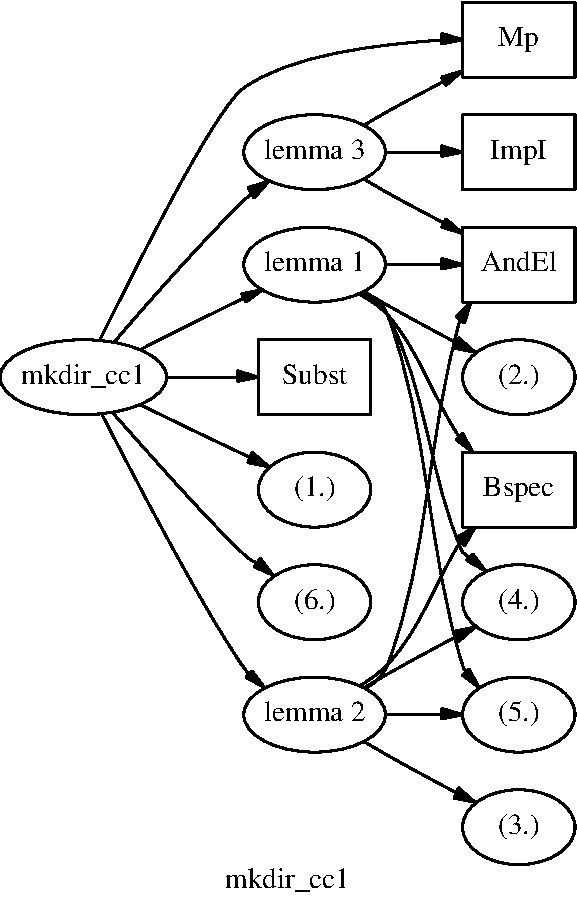
\includegraphics[]{pics/mkdir_cc1.pdf}}}
 %\epsfig{file=mkdir_cc1.ps,height=5.cm}
 \end{center}
 \caption{This is the lemmagraph for the manual proof of $mkdir\_cc1$. The basic rules are inside boxes, and both assumptions and facts found in the specification are printed as numbers.}
 \end{figure}
%
% 
% machine supported proof
%
The machine supported proof of $mkdir\_cc1$ using Isabelle98/HOL-Z can be grouped into five steps.

\begin{enumerate}
\item We formulated the proof obligations in Z. In doing so, the \Zeta~tool
  ensured usage of correct Z syntax and exported both the specification and the
  obligations to a valid HOL-Z format.
%
%
  \begin{center}
\begin{minipage}{.9\linewidth }
\ensuremath{mkdir\_cc}
\zcomment{\begin{zed}
mkdir\_cc1
== \forall mkdir @ \\
[
\Delta FileSystem; \Xi ProcessState; u? : Name | wdir \in \dom attributes
] 
\\
\end{zed}}
\end{minipage}
\end{center}
The HOL-Z \LaTeX\ style automatically generates a nice output of this condition. The following lines result from exporting it to Isabelle.
%
\begin{holzverb}
"mkdir_cc1 ==

      %A mkdir @ +..
                   %Delta SNAME FileSystem (attributes, files);
                   %Xi SNAME ProcessState (gid, uid, umask, wdir); 
                   u? setDecl Name
                 |--
                   wdir : dom attributes
                 -.." 
\end{holzverb}
%
Using this definition, we can start the Isabelle/HOL-Z proof:
\begin{holzverb}
zgoalw SysArchConsistency.thy [mkdir_cc1_def] "mkdir_cc1";
\end{holzverb}
For finding all function applications throughout the whole specification, we
used an ML function which prints each of them grouped by the Z structures where
they appear (zsection, axiomatic definition, schema definition, \dots)
\item In Isabelle/HOL-Z, we start with simplifying the goal by stripping off
  schema quantors and turnstyles and so on~(using \verb|stripS_tac|) and then
  continue by eliminating trivial set constraints which may be found in the
  assumptions either directly or via using a few minor rewrite steps (e.g.\
  expanding schemas).
\item At this point only showing $wdir \in \dom attributes$ is left to us. Using
  one substitution step and the fact $\dom files = \dom attributes$ from the
  predicate part of the $FileSystem$ schema, we reduce this to $wdir \in \dom
  files$.
\begin{holzverb}
by(res_inst_tac [("s","dom files"),("t","dom attributes")] subst 1);
\end{holzverb}
\item Reuse of outsourced lemmas allows us to achieve a higher degree of
  abstraction. The lemma $in\_dom\_if\_isdirin$ can be found in the library
  \verb|FileSystem.ML|.
%
%
\begin{holzverb}
 in_dom_if_isdirin
 =
   "[| ?f : Path -|-> Data + Unit; ?p : Path; (?p, ?f) : _isdirin_ |]
      ==> ?p : dom ?f"  
\end{holzverb}
%
\item The remaining subgoals can be erased trivially either directly or
  indirectly similarly as mentioned in step 2. One could envisage an ML function
  which tries solving a given goal by recursively expanding schemas (via depth-
  or breadth-first search) until the goal statement can be found or in case not,
  throws an exception. But this is a topic for future work.
\end{enumerate}
%
%
%
%
% [Deadlock-freeness section ]
%
%

\subsection{The Deadlock-freeness of the Operation Schemas}
Since the construction of these proof obligations (as described in the
introductory section of this chapter) is canonical, we will simply list the
condition formulations for all operations in the appendix. Some proofs are
contained in the in the HOL-Z distribution (see
\verb+examples/zeta/cvs-server/holz+). The proofs are non-trivial, because they
usually require to show that the state invariants (i.e.\  of
$FileSystem$,$ClientState$ and $RepositoryState$) are still valid after a chosen
system transition.
%
% (for each valid state s there has to exist a 
% successor state s' which preserves the state invariant
% , if transition s - op -> s' holds.)
%
%The proofs are
%highly non-trivial, since they usually require to show that the state invariants
%(i.e.  of $FileSystem$,$ClientState$ and $RepositoryState$) remain valid under
%transition.
%
%HH adds:
%
%
%
In this part, we will show a manual proof of the deadlock-freeness of the
operation $abs\_ci$ in the Z-Section $AbsOperations$ of the CVS Server
specification. Then we describe the computer-supported proof of the
deadlock-freeness of $abs\_ci$. We will see that it can be profitable to combine
manual and mechanized proofs.

With deadlock-freeness we mean that we want to ensure that no
operation possibly leads the system to a dead end. Hence we use the
goal formulation shown in the introductory part of this section. 

\zcomment{%
  \begin{schema}{abs\_ci}
    \Delta ClientState \\
    \Delta RepositoryState  \\
    files?: \power Abs\_Name \\
    \where
    (wfiles \cap files?) \subseteq \dom wc \\

    rep' = rep \oplus (\{ n: wfiles \cap files? | n \notin \dom rep \land n \in
    \dom wc\_uidtab \\
    \t1 \land (wc\_uidtab(n), abs\_passwd(wc\_uidtab~n)) \in
    \dom(authtab(rep))\} \dres wc') \\  
    \t2 \oplus (\{n : wfiles \cap files? | n \in \dom rep \land n \in \dom
    wc\_uidtab \\
    \t2 \land (wc\_uidtab(n), abs\_passwd(wc\_uidtab~n)) \in \dom(authtab~rep) \\
    \t2 \land (rep\_permtab(n),authtab(rep)(wc\_uidtab(n), \\
    \t2 abs\_passwd(wc\_uidtab~n)))\in cvs\_perm\_order\}
    \dres wc') \\

    rep\_permtab' = rep\_permtab \oplus \{ n: wfiles \cap files? |  n \notin
    \dom rep \land n \in \dom wc\_uidtab \\
    \t1 \land (wc\_uidtab(n), abs\_passwd(wc\_uidtab~n)) \in \dom(authtab~rep) @
    \\
    \t2 n \mapsto authtab(rep)(wc\_uidtab(n), abs\_passwd(wc\_uidtab~n)) \} \\

    \dom wc' = \dom wc \\
    wc\_uidtab' = wc\_uidtab \land abs\_passwd' = abs\_passwd \land wfiles' =
    wfiles \\ 
  \end{schema}}

%
% [goal abs_ci]
%
For this example, we will use the schema $abs\_ci$ which produces the
deadlock-free consistency condition $abs\_ci\_df\_cc$. This proof is done for
the previous version of the operation $abs\_ci$ shown above. The current version
defines $wc' = wc$ while the previous version uses nondeterminism for modelling
the successor state ($\dom wc' = \dom wc$). Since $wc' = wc$ implies $\dom wc'
= \dom wc$,
this proof holds for both versions.\\
\begin{center}
\mbox{abs\_ci\_df\_cc} $\equiv$
\begin{minipage}{5 cm}
\zcomment{\begin{schema}{syn\_pre(abs\_ci)}
  ClientState \\
  RepositoryState  \\
  files?: \power Abs\_Name \\
  \where
  (wfiles \cap files?) \subseteq \dom wc \\
\end{schema}}
\end{minipage}
$\implies
~\mbox{pre abs\_ci}$\\%
\end{center}
%
% [simplified goal abs_ci]
%
This proof goal can be simplified canceling those set constraints
that occur on both the left and right side of the implication.
\begin{center}
  \begin{minipage}{5 cm}
    \zcomment{\begin{schema}{syn\_pre(abs\_ci)}
      ClientState \\
      RepositoryState  \\
      files?: \power Abs\_Name \\
      \where
      (wfiles \cap files?) \subseteq \dom wc \\
    \end{schema}}
  \end{minipage}
  $\implies $%
~\mbox{pre }
  \begin{minipage}{5.5 cm}
    \zcomment{\begin{schema}{}
      ClientState' \\
      RepositoryState'  \\
      \where
      \dom wc' = \dom wc\\
      wc\_roletab' = wc\_roletab\\ 
      uid' = uid \land passwd' = passwd\\
      role' = role \land wfiles' = wfiles \\
    \end{schema}}
  \end{minipage}
\end{center}
%
% [common equation for pre]
%
After unfolding the definitions of pre and of the hiding operation, we can eliminate some existentially quantified variables trivially using the equations for the variables of the successor state. Note that we do not make any additional restrictions concerning the variable $wc'$. \\
%
% [unfolding pre OP]
%
\[
\mbox{pre(Op)} \stackrel{(def. pre)}{\equiv} \mbox{Op} \setminus (\mathbf{x'}, \mathbf{y!}) \stackrel{(def. hiding)}{\equiv} \exists \mathbf{x'} : \mathbf{t_1}; \mathbf{y!} : \mathbf{t_2} @ \mbox{Op}
\]
%
%
For the convenience of the reader, we unfold the definitions of $pre$ here.\\
%
% [further simplified goal abs_ci]
%
  \begin{minipage}{6cm}
  \zcomment{\begin{schema}{syn\_pre(abs\_ci)}
    ClientState \\
    RepositoryState  \\
    files?: \power Abs\_Name \\
    \where
    (wfiles \cap files?) \subseteq \dom wc \\
  \end{schema}}
\end{minipage}\hfill\\[-.5cm]
%\\[0.5cm]
\begin{tabular}{cccc}
{\Large$\implies$}&
$\begin{array}{l}
\exists~rep' : ABS\_DATATAB;\\
\quad rep\_permtab' : ABS\_PERMTAB;\\ 
\quad wc' : ABS\_DATATAB
\end{array}$
&$@$&
\parbox{3.8cm}{%
  \zcomment{\begin{schema}{}
    ClientState[wc'/wc]\\
    RepositoryState'  \\
    \where
    \dom wc' = \dom wc\\
  \end{schema}}}
\end{tabular}\\
First we show that the variables $rep'$, $rep\_permtab'$ and $wc'$ satisfy the
corresponding set constraints.\\
%
% two set costraints:
% (three, one directly)
%
\begin{center}
  \begin{enumerate}
        \item $rep' : ABS\_DATATAB$
        \item $rep\_permtab' : ABS\_PERMTAB$
        \item $wc' : ABS\_DATATAB$
  \end{enumerate}
\end{center}

With lemmas like $OplDom$ and $DomRestr$, these set constraints can be shown
easily.\\

\noindent\mbox{%
\begin{minipage}{0.97\textwidth}%
  \[
  \begin{prooftree}
        A:T \quad B:T \quad T=X \pfun Y
        \justifies
        (A \oplus B) : T
        \using
        \mbox{(OplDom)}
  \end{prooftree}
        \quad\quad%
  \begin{prooftree}
        R:T \quad T=X \pfun Y
        \justifies
        (A \dres R) : T 
        \using 
        \mbox{(DomRestr)}
  \end{prooftree}
  \]
\end{minipage}
%
%
}\\[0.4cm]
%-------------------------
%
By definition, the following holds :\\[0.3cm] $ABS\_DATATAB == Abs\_Name \pfun
Abs\_Data$\\
$ABS\_PERMTAB == Abs\_Name \pfun Cvs\_Perm$\\[0.3cm] The variables $rep'$ and
$rep\_permtab'$ are defined by equations using $rep$ and $rep\_permtab$
respectively. $wc'$ is given nondeterministically by the equation $\dom~wc' =
\dom~wc$. We may choose it according to this side condition. The syntactical
precondition yields $rep : ABS\_DATATAB$, $rep\_permtab : ABS\_PERMTAB$ and $wc
: ABS\_DATATAB$.
%
%

We still have to show the validity of the 4 predicates of $RepositoryState$ with $syn\_pre(abs\_ci)$ as assumption.\\
%
% [four subgoals]
%
%
\begin{center}
  \begin{enumerate}
  \item%
    $abs\_cvsauth \in \dom rep'$ 
  \item%
    $\dom rep' = \dom rep\_permtab'$ 
  \item%
    $rep\_permtab'(abs\_cvsauth) = cvs\_admin$ 
  \item%
    $rep'(abs\_cvsauth) \in \dom abs\_auth\_of$
  \end{enumerate}
\end{center}

The schema $syn\_pre(abs\_ci)$ contains the schema $RepositoryState$, we can access these four predicates using $rep$ instead of $rep'$ and $rep\_permtab$ instead of $rep\_permtab'$. The following equations for $rep'$ and $rep\_permtab'$ stem from the schema $abs\_ci$ and show how these variables are correlated. There still is some clearance, as the variable $wc'$ occurs on the right side of each of these equations. For readability, we introduce a few variables which allow highlighting of the important steps. \\[0,4cm]
%
% [variables + rep, rep_permtab]
%
\begin{tabular}{ccc}
  $rep\_new$ & $=$ & $(\{ n: wfiles \cap files? | n \notin \dom rep \land n \in
  \dom wc\_uidtab$ \\
  & & $\land (wc\_uidtab(n), abs\_passwd(wc\_uidtab~n)) \in
  \dom(authtab(rep))\} \dres wc')$\\
 & & \\
  $rep\_old$ & $=$ & $(\{n : wfiles \cap files? | n \in \dom rep \land n \in \dom
    wc\_uidtab $ \\
  & & $\land (wc\_uidtab(n), abs\_passwd(wc\_uidtab~n)) \in \dom(authtab~rep)$\\
  & & $\land (rep\_permtab(n),authtab(rep)(wc\_uidtab(n),$\\
  & & $abs\_passwd(wc\_uidtab~n)))\in cvs\_perm\_order\}
\dres wc')$\\
 & & \\
$rep\_permtab\_new$ & $=$ & $\{ n: wfiles \cap files? |  n \notin
    \dom rep \land n \in \dom wc\_uidtab$\\
 & & $\land (wc\_uidtab(n), abs\_passwd(wc\_uidtab~n)) \in \dom(authtab~rep) @$\\
 & & $n \mapsto authtab(rep)(wc\_uidtab(n), abs\_passwd(wc\_uidtab~n)) \}$\\

\end{tabular}\\[0.4cm]
\begin{tabular}{ccc}
 $rep'$ & $=$ & $(rep \oplus rep\_new \oplus rep\_old)$\\
 & & \\
 $rep\_permtab'$ & $=$ & $(rep\_permtab \oplus rep\_permtab\_new)$\\
\end{tabular}\\[0.4cm]
The fourth subgoal $rep'(abs\_cvsauth) \in \dom abs\_auth\_of$ cannot
be proven without adding further assumptions. We will prove the first
three subgoals in the following, and afterwards we will argue about
further measures concerning the fourth subgoal.
%
%
%
\subsubsection{Proof of the first Subgoal}
%
% [First Subgoal]
%
\[abs\_cvsauth \in \dom rep'\]
%
%
%
\label{proof:sg1}
Using the following statements, the first subgoal can be handled.\\
\begin{enumerate}
\item From the schema $RepositoryState$ in $syn\_pre(abs\_ci)$, we get
  the following fact:
\begin{center}
$abs\_cvsauth \in \dom rep$
\end{center}
\item We use the rules $(OplSubsDom)$, $(subsElem)$ and $(sTrans)$ in our proof:\\[0.4cm]
%
%
%
% fst, (OplSDom)
%
\begin{center}
\begin{minipage}{5 cm}%
  \[\begin{prooftree}%
   Y = X \oplus Z
   \justifies
    \dom X \subseteq \dom Y
   \using 
    \mbox{(OplSDom)}
  \end{prooftree}\]%
\end{minipage}\quad\quad%
%
% snd, (subsElem)
%
\begin{minipage}{5 cm}%
  \[\begin{prooftree}%
    x \in A
    \quad%
    A \subseteq B
  \justifies
  x \in B
  \using 
  \mbox{(SubsElem)}
\end{prooftree}\]%
\end{minipage} %
\end{center}
%
% thrd, (sTrans)
%
\begin{center}
\begin{minipage}{5 cm}%
  \[\begin{prooftree}%
    A \subseteq B
    \quad%
    B \subseteq C
  \justifies
    A \subseteq C
  \using 
  \mbox{(STrans)}
\end{prooftree}\]%
\end{minipage}\\
\end{center}
%
%
%
%
\item Applying $(OplSubsDom)$ twice on the definition of $rep'$, we can show:\\
\[
\begin{array}{rcl}
\dom rep &\stackrel{(OplSubsDom)}{\subseteq}& \dom (rep \oplus rep\_new)\\
&\stackrel{(OplSubsDom)}{\subseteq}& \dom (rep \oplus rep\_new \oplus rep\_old)\\
&\stackrel{(def.rep')}{\equiv}&\dom rep'
\end{array}
\]
\item Now, we can conclude:
\begin{center}
$(1.) abs\_cvsauth \in \dom rep \stackrel{(2)}{\implies} %
abs\_cvsauth \in \dom rep'$\\%
\end{center}%
\end{enumerate}\mbox{}
The following proof tree using natural deduction is a more detailed proof of the first subgoal.%
%
% prooftree for fst subgoal
%
\[%
\begin{prooftree}
  \[
  \mbox{(1.)}
  \justifies
  \parbox{2.1cm}{$abs\_cvsauth$ \\[0.1cm] 
   $\in \dom rep$ \vspace{0.1cm}}
  \]
  \quad 
  \[
    \[
      \[
      \mbox{(refl)}
      \justifies
       \parbox{2.8cm}{$rep \oplus rep\_neu$ \\[0.1cm]
        $= rep \oplus rep\_neu$\vspace{0.1cm}}
      \]
    \justifies
    \parbox{3.0cm}{$\dom rep \subseteq$ \\[0.1cm]
        $\dom (rep \oplus rep\_neu)$\vspace{0.1cm}}
    \using
    \mbox{(OplSDom)}
    \]
    \quad
    \[
      \[
      \mbox{(Def. $rep'$)}
      \justifies
      \parbox{2.0cm}{$rep' =  (rep$ \\[0.1cm] 
                $\oplus rep\_neu)$ \\[0.1cm]  
                $\oplus rep\_alt$ \vspace{0.1cm} }
      \]
    \justifies
    \parbox{2.0cm}{$\dom (rep$ \\[0.1cm] 
                $\,\oplus rep\_neu)$ \\[0.1cm]  
                $\subseteq \dom rep'$\vspace{0.1cm} }
    \using
    \mbox{(OplSDom)}
    \]
  \justifies
  \dom rep \subseteq \dom rep'
  \using
  \mbox{(STrans)}
  \]
  \justifies
  abs\_cvsauth \in \dom rep'
  \using
  \mbox{(SubsElem)}
\end{prooftree}
    \]%
%
%
%
\subsubsection{Proof-Setup for the second Subgoal}
%
% [Second Subgoal]
%
\[\dom rep' = \dom rep\_permtab'\]
%
%
%
%
% [rules, assumptions\ldots for second subgoal]
%
\label{proof:sg2}
The following proof for the second subgoal is more costly. Under the
global assumptions\\[0.4cm]
\begin{tabular}{cl}
$(A1)\quad\quad $ & $ (wfiles \cap files?) \subseteq \dom wc$\\
$(A2)\quad\quad $ & $ \dom rep = \dom rep\_permtab$\\
\end{tabular}\\[0.4cm]
and the side condition\\[0.4cm]
\begin{tabular}{cl}
$(SC)\quad\quad $ & $ \dom wc = \dom wc'$,\\
\end{tabular}\\[0.4cm]
we have to show : $\dom rep' = \dom rep\_permtab' $. Therefore we will use the following basic rules:\\[0.4cm]
\begin{tabular}{ll}
$(OplDomUn) \quad\quad $ & $ \dom (A \oplus B) = \dom A \cup \dom B$\\
$(UnKomm) \quad\quad $ & $ A \cup B = B \cup A$\\
$(UnAss) \quad\quad $ & $ (A \cup B) \cup C = A \cup (B \cup C)$\\
$(DresSub) $ & $ dom (A \dres B) \subseteq A $\\[0.3cm]
$(SubDres) $ &  
\begin{minipage}{6 cm}%
\[\begin{prooftree}%
  A \subseteq B
  \quad
  A \subseteq \dom C
  \justifies
  A \subseteq \dom (B \dres C)
\end{prooftree}\]
\end{minipage}\\[0.4cm]%
$(DomMaplet) $ & $ \dom \{a : S | P @ a \mapsto f(a)\} = \{a : S | P\}$\\
\end{tabular}\\[0.4cm]
We leave proving these basic rules as an exercise for the reader. The following lemmas are especially made for this proof:\\[0.4cm]
%
% [Lemmas for second subgoal]
%
\begin{tabular}{ll}
$\mbox{(L1)} \quad\quad $ & $ \dom rep = \dom rep \cup \dom rep\_old$\\[0.2cm]
$\mbox{(L2)} \quad\quad $ &  %
\begin{minipage}{6 cm}%
  \[\begin{prooftree}%
    \dom wc = \dom wc'%
    \quad%
    (wfiles \cap files?) \subseteq \dom wc%
  \justifies
  \dom rep\_new = \dom rep\_permtab\_new
\end{prooftree}\]%
\end{minipage}\\%
\end{tabular}\\[0.4cm]
In the next section, we show the lemmas (L1) and (L2), before we will continue with presenting the main proof.\\[0.4cm]
%
%
%
\subsubsection{Proof of Lemmas for the second Subgoal}
%
% [Lemmas for Second Subgoal]
%
%---
%
% [Lemma 1 for Second Subgoal]
%
\[\mbox{(L1)} \quad\quad \dom rep = \dom rep \cup \dom rep\_old\]

$rep\_old$ is defined as $C \dres wc'$. The set which we abbreviated with $C$ here, contains the conjunct $n \in \dom rep$. This implies that $C$ is a subset of $\dom rep$.\\
\[
\begin{array}{crcrcl}
(+) \quad\quad & \dom (C \dres wc')& \stackrel{(DresSub)}{\subseteq}& C &\stackrel{(C\subseteq\dom rep)}{\subseteq}& \dom rep\\
\end{array}
\]
With (+) we can complete the proof:
\[
\begin{array}{crcl}
\mbox{(L1)}& \dom rep \cup \dom rep\_old & \stackrel{(def. rep\_old)}{\equiv}& \dom rep \cup \dom (C \dres wc')\\
 & & \stackrel{(+)}{\equiv} & \dom rep\\
\end{array}%
\]
%
% [Lemma 2 for Second Subgoal]
%
Now we show the second lemma.
\[\mbox{(L2)} \quad\quad%
\begin{minipage}{6 cm}%
\[\begin{prooftree}%
    \dom wc = \dom wc'%
    \quad%
    (wfiles \cap files?) \subseteq \dom wc%
  \justifies
  \dom rep\_new = \dom rep\_permtab\_new
\end{prooftree}\]
\end{minipage}\\%
\]

Our proof for (L2) is organized in two parts:
%
\[\mbox{(a)} \quad\quad\dom rep\_new \subseteq \dom
rep\_permtab\_new\]
%
\[\mbox{(b)} \quad\quad\dom rep\_permtab\_new \subseteq \dom
rep\_new\]
%
In the following, we abbreviate the set $\{ n: wfiles \cap files? | n \notin \dom rep \land n \in \dom wc\_uidtab \land (wc\_uidtab(n), abs\_passwd(wc\_uidtab~n)) \in \dom(authtab(rep))\}$ with $D$.\\
Proof of (L2), (a):
%
% [Proof of (L 2)(a)
%
\[
\begin{array}{rcl}
\dom rep\_new & \stackrel{(def.rep\_new)}{\equiv}& \dom (D \dres wc')\\ 
& \stackrel{(DresSub)}{\subseteq} & \\
D & \stackrel{(DomMaplet)}{\equiv}& \dom rep\_perm\_tab\_new\\
\end{array}
\]
%
% [Proof of (L 2)(b)
%
Proof of (L2), part (b):\\
(L2) has two assumptions:\\[0.4cm]
\begin{tabular}{cl}
$(lSC)\quad\quad $ & $ \dom wc = \dom wc'$\\
$(lA1)\quad\quad $ & $ (wfiles \cap files?) \subseteq \dom wc$\\
\end{tabular}\\[0.4cm]
The assumption (lA1) is a local instance of (A1), and (lSC) is a local instance of (SC). Because of the constraint $(wfiles \cap files?)$ in the declaration part of $D$, it follows that $D \subseteq (wfiles \cap files?)$. \\
\[
\begin{array}{rcl}
\dom rep\_perm\_tab\_new &\stackrel{(DomMaplet)}{\equiv}& D \\ %
& \subseteq  & (wfiles \cap files?) \\%
&\stackrel{(lSC)}{\subseteq}& \dom wc \\ %
&\stackrel{(lA1)}{\equiv}& \dom wc'\\%
\end{array}
\]
Now we have:\\ 
\[\mbox{(*)}\quad\quad\dom rep\_perm\_tab\_new \subseteq \dom wc'\]
Using $\dom rep\_perm\_tab\_new \stackrel{(DomMaplet)}{\equiv} D$ we can conclude
\[\mbox{(**)}\quad\quad \dom rep\_permtab\_new \subseteq D\]
Applying the rule $(SubDres)$ unified with (*) and (**) as assumptions, we immediately get (L2)(b):\\[0.4cm]
\begin{tabular}{lclcr}
$\dom rep\_perm\_tab\_new$ & $\stackrel{(SubDres)}{\subseteq}$ & $ \dom(D \dres wc')$%
& $\stackrel{(def.rep\_new)}{\equiv}$ & $ \dom rep\_new$\\
\end{tabular}
%
%
%
\subsubsection{Main Proof of the second Subgoal}
%    
%  [main proof of second subgoal]
%   
Using the settings of the last but one section and the 2 lemmas (L1)
and (L2) proven in the section before, we can now present our main
proof for the second subgoal of the deadlock-free consistency
condition $abs\_ci\_df$.
\begin{center}
\begin{tabular}{rcl}
$\dom rep'$ &$\stackrel{(def. rep')}{\equiv}$&$  \dom (rep \oplus rep\_new \oplus rep\_old)$\\%
&$\stackrel{(OplDomUn)}{\equiv}$&$ \dom (rep \oplus rep\_new) \cup \dom rep\_old  $\\ %
&$\stackrel{(OplDomUn)}{\equiv}$&$ (\dom rep \cup \dom rep\_new) \cup \dom rep\_old$\\%
&$\stackrel{(UnKomm)}{\equiv}$&$ (\dom rep\_new \cup \dom rep) \cup \dom rep\_old$\\%
&$\stackrel{(UnAss)}{\equiv}$&$ \dom rep\_new \cup (\dom rep \cup \dom rep\_old)$\\%
&$\stackrel{(L1)}{\equiv}$&$ \dom rep\_new \cup \dom rep$\\%
&$\stackrel{(A2)}{\equiv}$&$ \dom rep\_new \cup \dom rep\_permtab$\\%
&$\stackrel{(L2,SC,A1)}{\equiv}$&$ \dom rep\_permtab\_new \cup \dom rep\_permtab$\\%
&$\stackrel{(UnKomm)}{\equiv}$&$ \dom rep\_permtab \cup \dom rep\_permtab\_new$\\%
&$\stackrel{(OplDomUn)}{\equiv}$&$ \dom (rep\_permtab \oplus rep\_permtab\_new)$\\%
&$\stackrel{(def.rep\_permtab')}{\equiv}$&$ \dom rep\_permtab'$\\%
\end{tabular}
\end{center}
%
%
%
\subsubsection{Proof of the third Subgoal}
%
\[rep\_permtab'(abs\_cvsauth) = cvs\_admin\]
%
%
%
%
% [Proof of third Subgoal]
%
%
\label{proof:sg3}
To prove the third subgoal of $abs\_ci\_df$, we need the following three arguments\\
\begin{enumerate}
\item Because of the definition of $rep\_permtab'$ in the schema $abs\_ci$, the following holds:\\
\begin{center}
$rep\_permtab' = rep\_permtab \oplus rep\_permtab\_new$
\end{center}
\item The schema $RepositoryState$ inside of $syn\_pre(abs\_ci)$ has the following item in its schema declaration part:\\
\begin{center}
$abs\_cvsauth \in \dom rep$
\\
\end{center}
The set $rep\_permtab\_new$ has the conjunct $n \notin \dom rep$ in its predicate
part. We can conclude that the tuple ($abs\_cvsauth$, $?X$) in $rep\_permtab$
will not be overwritten. We use lemma $ApplOpl$ to express this.\\

%
\noindent\mbox{%
\begin{minipage}{0.97\textwidth}%
  \[
  \begin{prooftree}
        x \notin \dom S
        \justifies
        (R \oplus S)~x = R~x
        \using
        \mbox{(ApplOpl)}
  \end{prooftree}
  \]
\end{minipage}}%
%

\item This item can also be found in $RepositoryState$ from $syn\_pre(abs\_ci)$:\\
\begin{center}
$rep\_permtab(abs\_cvsauth) = cvs\_admin$
\end{center}
\end{enumerate}

Using the facts accumulated above, we can state this proof:\\

\begin{tabular}{lcc}
$rep\_permtab'(abs\_cvsauth) $ & $\stackrel{(1)}{\equiv}$ & $ (rep\_permtab \oplus rep\_permtab\_new)~abs\_cvsauth$\\
  & $\stackrel{(2)}{\equiv}$ & $ rep\_permtab~abs\_cvsauth$\\
  & $\stackrel{(3)}{\equiv}$ & $ cvs\_admin$\\
\end{tabular}
%
%
%
\subsubsection{Unprovable fourth Subgoal}
%
% [Fourth Subgoal]
%
\[rep'(abs\_cvsauth) \in \dom abs\_auth\_of\]\label{proof:sg4}
%
%
%
Without adding assumptions, the fourth subgoal cannot be proved, assuming we
have a consistent underlying theory (see first section of this chapter). The
$abs\_ci$ operation possibly leads the system to a deadlock.  The predicate
$rep'(abs\_cvsauth) \in \dom abs\_auth\_of$ means that after executing an
$abs\_ci$ operation, the actual version of the file $abs\_cvsauth$ in the
repository has to lie in the domain of the authentication table $abs\_auth\_of$.
This statement is not so profound because in this configuration of the CVS-server
only with $perm = cvs\_admin$ the commit operation will start. The schema
$RepositoryState$ contains the condition $rep\_permtab(abs\_cvsauth) =
cvs\_admin$ which ensures this. If we trust the users having $perm =
cvs\_admin$, we can simply add this assumption. Otherwise we could write a
script which also ensures this: before allowing a commit on the file
$abs\_cvsauth$, we simply check if the new version is still parseable, and in
case not, continue with the old version.
%
% (without the following empty line:
% the image is shifted to the right)
\begin{figure}%
\rotatebox{0}{\scalebox{0.8}{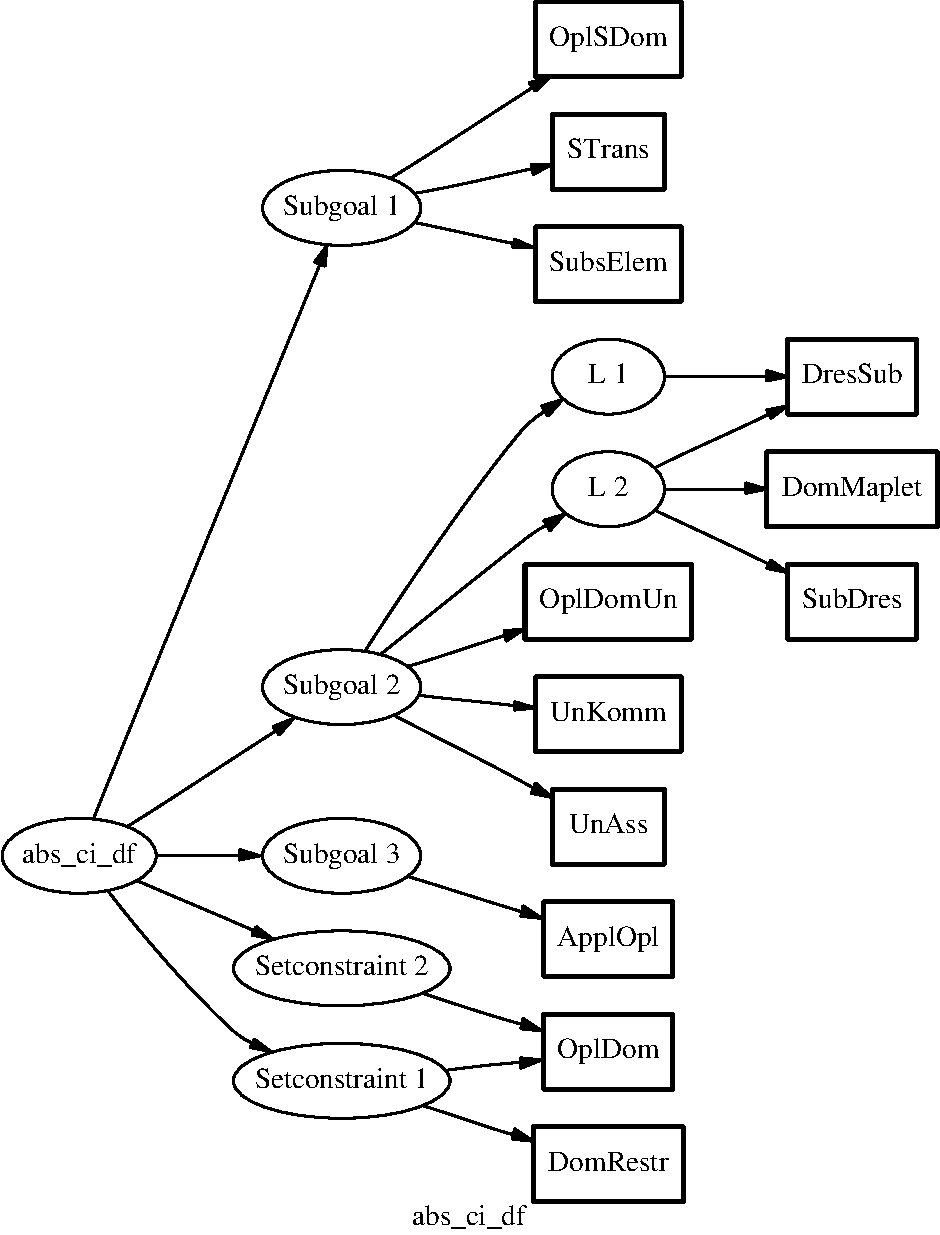
\includegraphics[]{pics/abs_ci_df_Graph_man.pdf}}}
\caption{A lemmagraph for the manual proof of $abs\_ci\_df$}%
\end{figure}%
%
%
%
\subsubsection{Computer Supported Proof}
%
% [Computer Supported Proof]
%
As mentioned at the beginning of this section, proofs of deadlock-free
consistency conditions can get arbitrarily hard to handle. To complete such a
task, we will see that it is profitable to use a mechanical proof. Although a
paper and pencil proof is essential, automatic simplification and management of
assumptions, side conditions (to name just a few examples) can significantly
reduce the required time and
increase trust in the stability of it.\\
The manual proof we have shown has been the basis for the computer supported
proof. The idea of having side conditions in a proof is realised implicitly by
the theorem prover. Completing the goal with the additional assumption
$rep'(abs\_cvsauth) \in \dom abs\_auth\_of$ is a mixture of redrawing the proof
shown before and using simplification routines and automatic tactics. Using and
improving a lemma library and gathering subtasks combining tacticals and
ML-functions leads to a
remarkably fast and short result.\\

Given a syntactic precondition, the goals can be generated uniformly using the HOL-Z-\LaTeX-style.\\[0.4cm]
%
% orginal (modified a little):
%
% (zcomment + naming)
%
\newsavebox{\sampleAbsCiDFBox}
\begin{lrbox}{\sampleAbsCiDFBox}
\begin{minipage}{.9\linewidth}
\ensuremath {abs\_ci\_df}\hfill \\
\zcomment{\begin {dzed}
abs\_ci\_df == 
[ClientState; RepositoryState; files? : \power Abs\_Name | (wfiles \cap files?) \subseteq \dom wc]
\implies \pre abs\_ci
\end{dzed}}
\end{minipage}
\end{lrbox}
\newcommand{\sampleAbsCiDF}{\usebox{\sampleAbsCiDFBox }}
%
% now, use it:
\sampleAbsCiDF\mbox{}\\[0.4cm]
%
%
%
To give an overview, we also add the lemmagraph of the Isabelle proof.
Sometimes, we needed slightly different instances of the lemmas used in the
manual proof. The machine supported proof has been constructed top down. At
first, the main lemmas were proven. Then the main proof was built
linking the lemmas by backward reasoning. Some steps mentioned in
the manual proof were proven automatically.
% 
% 
\begin{figure}%
\rotatebox{0}{\scalebox{0.8}{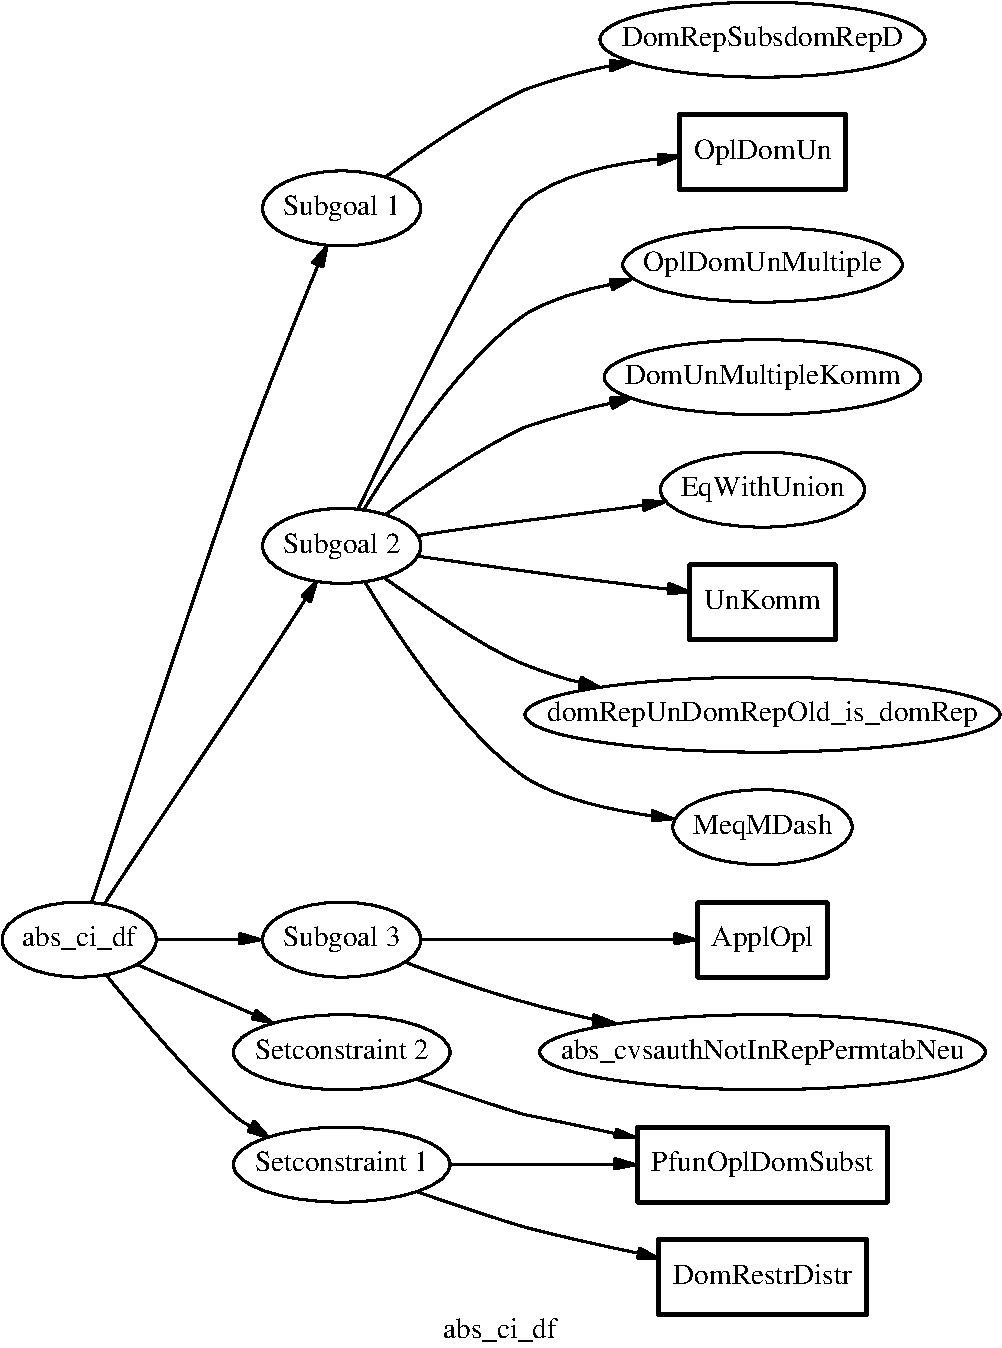
\includegraphics[]{pics/abs_ci_df_Graph.pdf}}}
\caption{A lemmagraph for the proof of $abs\_ci\_df$ using Isabelle/HOL-Z}%
\end{figure}%
%
%
% 
%
\newpage

\section{Verifying the Refinement}
\label{sec:refinement}

\zsection[AbsOperations,CVSServer]{Refinement}\vspace{1ex}\noindent

In this section, we focus on the refinement of the data types of our abstract
system architecture to data structures of our concrete implementation
architecture.  In particular, we will map the CVS repository and working copy to
a \unix file system and permissions to file attributes.

In order to prove that the concrete data structures correctly implements the
abstract data types, we have to define an abstraction schema $R$ which relates
the components of the abstract state schemas to the components of the concrete
implementation state schemas and thereby explains which concrete states
represent which abstract states.

The definition of this relating schema needs auxiliary functions $Rdata$ and
$Rname2path$ that map abstract data to concrete data, i.e.\ files, and the
abstract names of files to paths in the \unix file system.  Since we are not
concerned about the content of the files (except the administration files of
CVS), a very rough specification of these functions suffices.
\begin{axdef}
  Rdata: Abs\_Data \bij Data \\
  Rname2path: Abs\_Name \bij Path \\
  \where
% FRANK: was soll das?
%  \forall p: \ran Rname2path @ cvs\_rep \prefix p \\
  Rname2path(abs\_cvsauth) = cvs\_rep \cat \langle CVSROOT, cvsauth \rangle \\
\end{axdef}

Now we can proceed to define the abstraction schema $R$.  Importing the abstract
and concrete state schemas introduces all components that have to be set into
relation.  Note that some components ($cvs\_uid$ or $passwd$ for example) of the
abstract state also appear in the concrete state.  These components have the
same meaning in both states and do not need to be related in this schema.  The
set $wfiles$ of names of the abstract state, which is used to control the access
operations, must be related to the concrete working directory $wdir$.
Furthermore, we require that the files in the working copy $wc$ and in the
repository $rep$ of the abstract state have corresponding files in the
appropriate directories of the concrete file system $files$.  We also require
that the permission tables in the abstract and in the concrete state are the
same and that the roles and passwords that are assigned to each file in the
working copy of the abstract state have corresponding attributes in the concrete
state.
\begin{schema}{R}
  ClientState \\
  RepositoryState \\
  ProcessState \\
  Cvs\_FileSystem \\
  \where
  abs\_passwd = cvs\_passwd \\

  \forall n: wfiles @ wdir \prefix Rname2path(n) \\
  
  Rname2path \limg \dom wc \rimg = \dom wcs\_attributes \\

  authtab(rep) = get\_auth\_tab(files) \\
  \forall n: \dom rep @ \exists f: \dom files@ cvs\_rep \prefix f \\
  \t1 \land Rname2path(n) = f \land Inl(Rdata(rep~n)) = files(f) \\
  \forall n: \dom wc @ wc\_uidtab(n) = ((wcs\_attributes(Rname2path~n)).f\_uid)  \\
  \forall n: \dom wc @ \exists f: \dom files @ \lnot (cvs\_rep \prefix f) \\
  \forall f: \dom rep @ \exists ps: \power Perm | \{ru,rg\} \subseteq ps @ \\
  \t1 attributes(Rname2path~f) = \lbind \< perm == ps, \\
  uid == cvsperm2uid(rep\_permtab~f), \\
  gid == cvsperm2gid(rep\_permtab~f) \rbind \>
\end{schema}

Closely following the refinement notion of Spivey~\cite{spivey:z_notation:1992},
we must prove two refinement conditions for each operation on the abstract state
$\sigma_{abs}$ and its corresponding operation on the concrete state
$\sigma_{conc}$.  However, the original setting assumes that the abstract
operation $op_{abs}$ and the corresponding concrete operation $op_{conc}$ are
defined over the same input and output parameters, which does not always hold
for our operations.  Therefore, we extend the original refinement notion by
(sometimes) strengthening the premises of the refinement conditions.

\paragraph{Refinement condition (I1)}
A concrete operation $op_{conc}$ can make a transition whenever its
corresponding abstract operation $op_{abs}$ can make a transition (i.e.\ a
successor state $\sigma'_{conc}$ exists). The situation is depicted in
Figure~\ref{fig:refcon1}.
\begin{figure}[h!]
    \center
      \scalebox{0.5}{\input{pics/ref_concept1}}
    \caption{Refinement Condition (I1).\label{fig:refcon1}}
\end{figure}

In other words, condition (I1) ensures that a concrete operation terminates
whenever its corresponding abstract operation is guaranteed to terminate. For
input parameters $in?$, this is formalized as:
\zcomment{
  \begin{zed}
    \forall \sigma_{abs}; \sigma_{conc}; in?: T_1 @ \pre op_{abs} \land R
    \implies \pre op_{conc} \\ 
  \end{zed}}


\paragraph{Refinement condition (I2)}
For any possible state $\sigma'_{conc}$ reachable by the concrete operation,
there must be a $R$-related state $\sigma'_{abs}$ that can be reached by the
abstract operation, provided that the initial states $\sigma_{abs}$ and
$\sigma_{conc}$ had been $R$-related. The situation is depicted in
Figure~\ref{fig:refcon2}.
\begin{figure}[h!]
    \center
      \scalebox{0.5}{\input{pics/ref_concept2}}
    \caption{Refinement Condition (I2).\label{fig:refcon2}}
\end{figure}

This condition ensures that the state after the concrete operation represents
one of those abstract states in which the abstract operation could terminate.
For input parameters $in?$ and output parameters $out!$, this is represented
formally:
\zcomment{
  \begin{zed}
    \forall \sigma_{abs}; \sigma_{conc}; \sigma'_{conc}; in?: T_1; out!: T_2
    @ \\
    \t1 \pre op_{abs} \land R \land op_{conc} \implies (\exists
    \sigma'_{abs} @ R' \land op_{abs}) \\
  \end{zed}}
  
Additionally, there is the requirement that the initial states are compatible:
\paragraph{Refinement condition (II)}
Each possible initial state of the concrete type must represent a possible
initial state of the abstract type.
\zcomment{
  \begin{zed}
    \forall \sigma_{conc} @ Init_{conc} \implies (\exists \sigma_{abs} @
    Init_{abs} \land R) \\
  \end{zed}}

In the following subsections, we will list the proof obligations for the
refinement in full detail. The proofs can be found in the in the HOL-Z
distribution (see \verb+examples/zeta/cvs-server/holz+). The proofs are highly
non-trivial.

%\subsection{Examples of Refinement}

%\subsubsection{Refinement of the initial states}
%The initialization schemas for the abstract and concrete state are
%missing.\fixme{FRANK: Initialzustaende fehlen noch!}

\subsection{The login operation}
As a first simple example, we show the two conditions (I1) and (I2) for the CVS
\cvscmd{login} command, which is used to initially authenticate a client to the
CVS server.  For the definition of the operation schemas, we refer to the
$abs\_login$ schema in the abstract section, and the $cvs\_login$ schema in the
implementation section.

We need the additional preconditions that the requested role and the supplied
passwords are the same on the abstract and concrete level. Here, we
intentionally did not give the input parameters the same names since this leads
to problems in the generated refinement proof-obligations; the standard
refinement notion implicitly requires abstract and concrete states to have
distinct bindings. Since we cannot use arbitrary formulas in schema calculus
expressions, we must wrap a schema $Asm\_login$ around these preconditions:
\begin{schema}{Asm\_login}
  passwd?, cvs\_pwd?: Cvs\_Passwd \\   
  uid?, cvs\_uid?: Cvs\_Uid \\
  \where
  passwd? = cvs\_pwd? \land uid? = cvs\_uid? \\
\end{schema}


\begin{schema}{pre\_of\_cvs\_login}
  files: FILESYS\_TAB \\
  cvs\_uid?: Cvs\_Uid \\
  cvs\_pwd?: Cvs\_Passwd \\
  \where
  (cvs\_uid?,cvs\_pwd?) \in \dom(get\_auth\_tab~files) \\
\end{schema}
\begin{schema}{pre\_of\_abs\_login}
  uid?: Cvs\_Uid \\
  passwd?: Cvs\_Passwd \\
  rep: ABS\_DATATAB \\
  \where
  (uid?,passwd?) \in \dom(authtab~rep) \\
\end{schema}

\begin{axdef}
  PreLogin: \nat \\
  \where
  \forall Cvs\_FileSystem; ProcessState; Cvs\_FileSystem '; ProcessState '; \\
  \t1 cvs\_uid?: Cvs\_Uid; cvs\_pwd?: Cvs\_Passwd @ \\
  \t2 pre\_of\_cvs\_login \implies \pre cvs\_login \\

  \forall ClientState; RepositoryState; ClientState '; RepositoryState '; \\
  \t1 uid?: Cvs\_Uid; passwd?: Cvs\_Passwd @
  pre\_of\_abs\_login \implies \pre abs\_login \\
\end{axdef}

%%adb
\zrefinesOp[Astate={ClientState,RepositoryState},
            Cstate={ProcessState,Cvs\string\_FileSystem},
            Aop=abs\string\_login,
            Cop=cvs\string\_login,
            Args={passwd?: Cvs\string\_Passwd, cvs\string\_pwd?:
            Cvs\string\_Passwd, uid?: Cvs\string\_Uid, cvs\string\_uid?: 
            Cvs\string\_Uid}, 
            Abs=R,
            Assumption=Asm\string\_login,
            display
            ]{login}


\subsection{The add operation}

\begin{schema}{Asm\_add}
  p?: Path \\
  newfiles?: ABS\_DATATAB \\
  wdir: Path \\
  \where
  \forall n: \dom newfiles? @ wdir \cat p? \prefix Rname2path(n) \\
\end{schema}

\zrefinesOp[Astate={ClientState,RepositoryState},
            Cstate={ProcessState,Cvs\string\_FileSystem},
            Aop=abs\string\_add,
            Cop=cvs\string\_add,
            Args={newfiles?: ABS\string\_DATATAB; p?: Path},
            Abs=R,
            Assumption=Asm\string\_add,
            display
            ]{add}



\subsection{The update operation}

\begin{schema}{Asm\_update}
  p?: Path \\
  files?: \power Abs\_Name \\
  wdir: Path \\
  \where
  \forall n: files? @ wdir \cat p? \prefix Rname2path(n) \\
\end{schema}


\begin{schema}{pre\_of\_cvsUp}
  p?: Path \\
  files: FILESYS\_TAB \\
  wcs\_attributes: CVS\_ATTR\_TAB \\
  wdir: Path \\
  uid: Uid \\
  attributes: FILEATTR\_TAB \\
  \where
  cvs\_rep \cat repOf(wcs\_attributes~wdir) \cat p? \in \dom files \\
  has\_w\_access(uid, wdir \cat p?, attributes) \\
\end{schema}
\begin{schema}{pre\_of\_cvsUpErr}
  p?: Path \\
  wdir: Path \\
  uid: Uid \\
  attributes: FILEATTR\_TAB \\
  \where
  \lnot (has\_w\_access(uid, wdir \cat p?, attributes)) \\
\end{schema}
\begin{schema}{pre\_of\_cvsUpNoAct}
  p?: Path \\
  files: FILESYS\_TAB \\
  wcs\_attributes: CVS\_ATTR\_TAB \\
  wdir: Path \\
  uid: Uid \\
  attributes: FILEATTR\_TAB \\
  \where
  cvs\_rep \cat repOf(wcs\_attributes~wdir) \cat p? \notin \dom files \\
\end{schema}
\begin{axdef}
  PreUpdate: \nat \\
  \where
  \forall Cvs\_FileSystem; ProcessState; Cvs\_FileSystem '; ProcessState '; \\
  \t1 p?: Path; files: FILESYS\_TAB; wcs\_attributes: CVS\_ATTR\_TAB; \\
  \t1 wdir: Path; uid: Uid; attributes: FILEATTR\_TAB; error!: \denotation @ \\
  \t2 pre\_of\_cvsUp \implies \pre cvsUp \\

  \forall Cvs\_FileSystem; ProcessState; Cvs\_FileSystem '; ProcessState '; \\
  \t1 p?: Path; files: FILESYS\_TAB; wcs\_attributes: CVS\_ATTR\_TAB; \\
  \t1 wdir: Path; uid: Uid; attributes: FILEATTR\_TAB; error!: \denotation @ \\
  \t2 pre\_of\_cvsUpNoAct \implies \pre cvsUpNoAct \\

  \forall Cvs\_FileSystem; ProcessState; Cvs\_FileSystem '; ProcessState '; \\
  \t1 p?: Path; files: FILESYS\_TAB; wcs\_attributes: CVS\_ATTR\_TAB; \\
  \t1 wdir: Path; uid: Uid; attributes: FILEATTR\_TAB; error!: \denotation @ \\
  \t2 pre\_of\_cvsUpErr \implies \pre cvsUpErr \\
\end{axdef}

\zrefinesOp[Astate={ClientState,RepositoryState},
            Cstate={ProcessState,Cvs\string\_FileSystem},
            Aop=abs\string\_up,
            Cop=cvs\string\_update,
            Args={p?: Path; files?: \string\power\space Abs\string\_Name},
            Abs=R,
            Assumption=Asm\string\_update,
            display
            ]{update}

\subsection{The commit operation}

The schema $Asm\_ci$ defines the assumption that the current user has read
access to the working directory.  This must be stated in a separate assumption
because the abstract state has no notion of read/write/execute rights on files.
\begin{schema}{Asm\_ci}
  uid: Uid \\
  wdir: Path \\
  attributes: FILEATTR\_TAB \\
  p?: Path \\
  files?: \power Abs\_Name \\
  \where
  has\_r\_access(uid, wdir \cat p?, attributes) \\
  \forall n: files? @ wdir \cat p? \prefix Rname2path(n) \\
\end{schema}
\noindent With the assumptions in $Asm\_ci$ we can now formulate the refinement
proof obligations for the commit operations:

\zrefinesOp[Astate={ClientState,RepositoryState},
            Cstate={ProcessState,Cvs\string\_FileSystem},
            Aop=abs\string\_ci,
            Cop=cvs\string\_ci,
            Args={p?: Path; files?: \string\power\space Abs\string\_Name},
            Abs=R,
            Assumption=Asm\string\_ci,
            display
            ]{ci}

\subsection{The cd operation}

To relate the parameters of the abstract and the concrete $cd$ operation, we
define the schema $Asm\_cd$.  We require that all abstract files, which are to
be focused ($wfiles?$) must be related to a concrete file within the current
working directory $wdir$ (appended by some path $p?$) or one of its
subdirectories.

Setting the focus to a set of files in the abstract model corresponds to setting
the working directory (which also represents a set of files, namely all files
within it or within one of its subdirectories).
\begin{schema}{Asm\_cd}
  wfiles?: \power Abs\_Name \\
  p?, wdir: Path \\
  \where
  \forall n: wfiles? @ wdir \cat p? \prefix Rname2path(n) \\
\end{schema}
\noindent For this operation it suffices to only take $FileSystem$ into account,
not $Cvs\_Filesystem$.

\zrefinesOp[Astate={ClientState,RepositoryState},
            Cstate={ProcessState,FileSystem},
            Aop=abs\string\_cd,
            Cop=cd,
            Args={p?: Path; wfiles?: \string\power\space Abs\string\_Name},
            Abs=R,
            Assumption=Asm\string\_cd,
            display
            ]{cd}




%%% Local Variables:
%%% TeX-master: "arch"
%%% fill-column:80
%%% x-symbol-8bits:nil
%%% End:

% LocalWords:  conservativity conjoints


%% SECTION
\section{Analysis} \label{sec:analysis}

In this section, we describe the analysis of our, and hence the OMG's
specification.


\subsection{Attacker scenarios}
\label{sec:attacker}

In this section, we define some attacker scenarios which help us guide the
analysis process.

\begin{itemize}
\item an attacker may insert a malicious object
\item someone calls legal operations with illegal parameters
\item can an attacker gain access to the internal data of an ORB
\item security association
\item attack against the interface repository
\item interception of communication between ORBs and/or objects
\item difference between security aware and unaware applications
\end{itemize}


\rcsInfo $Id: conclusion.tex,v 1.14 2003/12/04 15:03:06 brucker Exp $

\chapter{Conclusion}

We presented a case-study where an access control security problem for a
realistic system has been made amenable to formal, machine-based analysis. As a
hidden theme, we also presented a \emph{method} for analyzing security in
off-the-shelve operating system environments: First, specify the security
architecture (as a framework for formal security properties), second, specify
the implementation architecture (validated by inspecting informal specifications
or code and by testing), third, set up the security technology mapping as a
refinement problem, forth, establish a formal security analysis over the
transitive closure over the system transition relation, and fifth, prove
refinements and security properties by mechanized, gap-less proofs. This method
is applicable for a wider range of security problems and may be relevant, e.g.,
in mission critical e-commerce applications or in e-government applications,
where high-level certifications are mandatory.

More precisely, we have mapped an abstract model of the CVS-Server (with the
access-control model RBAC inside) to a more concrete implementation model based
on the concrete security mechanisms as offered by the traditional UNIX/POSIX
security architecture. Moreover, we also provided an implementation in form of a
configuration of the standard off-the-shelf implementation of
CVS~\cite{cvshome:2001}.  Thus, we showed an application of formal methods for
the field of security implementations, both from the technical and the
conceptual side. In the sequel, we will discuss these aspects in more detail.

\section{The Technical Side: A Secure CVS Configuration}
Our formal model (and its analysis) built the foundation of ``our'' CVS server
setup in our group at the University of Freiburg. At present, it is applied for
a repository containing $2.5$ Gigabyte of data for over $80$ users categorized
in five roles.

The presented setup addresses our main requirements: it does not monopolize an
additional machine with the CVS service, which would result in special
administration and installation of it, and it enforces a highly desirable access
control model. Moreover, any machine in our network can be assigned to our CVS
service, without any loss in security. Our CVS-server implementation requires
only the standard access control policy provided by the Unix standard, i.e.\ there
is no need for e.g.\ access control lists (ACL) as provided by some Unix
variants. Further, our implementation guarantees the encrypted transmission of
the passwords and the versioned data (not discussed in this report).

The main disadvantage for the users is the need for a special (patched) CVS
client, which also leads to some additional administrative work, because we have
to distribute these clients in source code and as binary for different operation
systems. Further, the security policy is `hard-wired' into our setup, e.g.\ 
support for write exclusion within one CVS role is realized via a different
mechanism.

\subsection{Related Work}
Other approaches for securing the standard CVS client/server model (using the
\texttt{pserver}-protocol) can roughly be divided into four classes:
\begin{enumerate}
\item Securing authentication and network traffic by providing SSL
  support, e.g.\ via tunneling~\cite{berezin:tunnel:2001} or wrapping
  the standard CVS server~\cite{vogt:cvsauth:2001},
\item Protecting the local network by running the standard CVS server in a
  sandbox (chrooted) environment~\cite{hess:anonymous:2001,idealx:chroot:2001},
\item Re-engineering the implementation of the
  \texttt{pserver}-protocol~\cite{nserver},
\item Setting up large scale closed servers providing CVS functionality, together with
  a project administration ~\cite{fsf:savannah:2001,osdn:sourceforge:2001}.
\end{enumerate}
These solutions mainly attempt to fix the known problems with the standard
CVS implementation by either providing encryption or minimizing the harms of a
intruder.  Whereas this is clearly one part of our problem, we also wanted to
provide an access control model, which lead to our choice
of~\cite{vogt:cvsauth:2001} as basis for our work, which solves the vital
problem of authentication and encryption of data transmission. Our DAC based
RBAC setup is an add-on on top of that, such that our setup can be used
together with most of the other approaches listed above.
\subsection{Future Work}
In our opinion, the greatest improvement of our CVS-server setup would be the
support of more flexible access control policies. Our implementation supports
already write exclusion within a CVS permission via a script\footnote{This script,
  called \texttt{cvs\_acls}, is part of the standard CVS distribution and can be
  found in the \texttt{contrib} directory.} implementing ACLs (access control
lists). Whereas such a write exclusion support clearly opens the door for
generic access policies its success is clearly limited by the lack of generic
hooks for implementing security checks (see for example~\cite{Linux-LSM} for
such an interface). Therefore any effort implementing a generic access control
into CVS (without rewriting the CVS system) would either lead to a complex and
intransparent configuration or it would heavily depend on the
underlying operation system (e.g.\ ACLs of the underlying filesystem), or both.

Taking all the well known hassles (e.g.\ moving of files, \ldots) of CVS into
account, we see a great future for projects creating a \emph{successor} of
CVS\@. Candidates for a replacement --- we only mention
Subversion~\cite{subversion} and OpenCM~\cite{opencm} here --- are taking long
strides toward production use. Subversion can be considered as the natural choice,
since it aims to solve the problems of CVS on the version control side
and supports a fine grain access control model using WebDAV~\cite{} in the future.
On the other side, OpenCM was designed with a refined access control mechanism
beyond RBAC from the beginning, but is weaker as a version control system.

Concluding, when setting up a \emph{new} version control system in the near
future, we would probably use one the CVS successors. We would favor
Subversion over OpenCM because of its better support in the free software
community and our relatively modest demands with respect to access
control.

\section{The Conceptual Side: Formal Methods for Security Technology}

It has been widely recognized that security properties can not be easily refined
--- actually, finding refinement notions that preserve security properties are a
hot research topic. However, standard refinement proof technology has still its
value here since it checks that abstract security requirements (which can be
seen as \emph{security against unintentional misuse}) are indeed achieved by a
mapping to concrete security technology, and that implicit assumptions on this
implementation have been made explicit. With respect to security against
\emph{intentional exploits of security leaks}, we believe that specialized
refinement notions will be limited to restricted aspects of a system. For this
problem, in most cases the answer will be to analyze the security on the
implementation level, possibly by reusing results from the abstract level. From
the methodological viewpoint this simply means that for an analysis of
\emph{intentional exploits of security leaks} implementation architectures must
simply be taken more seriously, which implies that more detailed and
implementation oriented models deserve more attention as before, where more
abstract models have been preferred. But in security analysis, more abstract
models are not necessarily better ones.

It is characteristic for our approach to consider security properties like
access control as ordinary functional properties; as a consequence, the
classical distinction between security and safety is very often difficult to
establish within our model. When refining a security architecture down
to an
implementation architecture, it is merely tradition to consider one form of
exceptional behavior (e.g.\ precondition that $has\_w\_access$ holds for a user
and a file) as security and another form (e.g.\ a path has the right format and
enables indeed to access a file in the filesystem) as safety.

\subsection{Related Work}

\begin{enumerate}
\item The common reference for stating that security properties (i.e.\ 
  information flow) are incompatible with refinement
  is~\cite{jacobs:derivation:1998}, where also a first method for stepwise
  development is proposed. More recent work for information flow
  is~\cite{Mantel:inp:2001} (where also a nice overview can be found). Other
  recent work on security-preserving refinements
  are~\cite{juerjens:secrecy-preserving:2001} (secrecy)
  and~\cite{santen:confidentiality-preserving:2002} (confidentiality).  To all
  these approaches, the critique above applies: these notion are focused on one
  particular security notion (so the question on combination arises), the
  transition to ``realistic'' implementations is not handled, such that these
  techniques remain limited to special aspects of a system.
\item Sandhu already described in~\cite{sandhu.ea:decentralized:1998} a method
  for embedding Role-Based Access Control with the Discretionary Access Control
  provided by standard \unix{} systems. Our implementation used this
  construction for providing the static role.
\item To our knowledge, there is amazingly few work on formalizing
  the UNIX/POSIX filesystem in the literature. Some approaches focus
  on the functional
  aspects~\cite{heisel:specification:1995,morgan.ea:unix-filesystem:1984}.
  The model in the Isabelle/HOL distribution by Markus Wenzel copes
  with security aspects and has inevitably many similarities with ours;
  however, it does not handle the execution flag, groups, not to
  mention the set-bits which play an important role in the role
  propagation when creating subdirectories.
 \end{enumerate}
\subsection{Future Work}
The formal proofs we did so far represent in our opinion a ``proof of
technology'' for this type of reasoning, but we do not claim that they represent
a thorough and complete analysis of the (real) CVS-server. So far, most
consistency, but only selected refinement and security properties have been proven.

However, from our experience gained by our proofs, we believe that specialized
proof technologies for certain types of proofs (refinement, security-properties)
in our methodological frame and concrete proof-technology can be improved and
will lead --- together with more and extended standard models for operating
system interfaces --- will dramatically increase the effectivity and feasibility
of our approach.


%%% Local Variables:
%%% TeX-master: "arch"
%%% fill-column:80
%%% x-symbol-8bits:nil
%%% End:



%%%%%%%%%%%%%%%%%%%%%%%%%
%% Appendix            %%
%%%%%%%%%%%%%%%%%%%%%%%%%
\appendix
\cleardoublepage
\part*{\Huge\textbf{Appendix}}
\rcsInfo $Id: appendix.tex,v 1.25 2003/10/21 11:43:36 hiss Exp $

\chapter{An Example CVS server setup}\label{cha:textsfs-repos}
In this chapter, we give a short description of ``our'' CVS server
setup (see Fig.~\ref{fig:mapping} for an overview) for the software 
engineering group at the University
Freiburg. We only describe the specific setup of the used tools, for a 
comprehensive understanding one should also read the manuals~\cite{vogt:cvsauth:2001,cederqvist.ea:cvs:2000, miller:sudo:2002, frisch:administration:1995} of the used tools.
\begin{figure}
  \center
    \scalebox{0.4}{\input{pics/mapping_overview}}
    \caption{The general idea/overview for the mapping.\label{fig:mapping}}
\end{figure}

\section{Motivation}
\subsection{Our Requirements}
We needed a reliable CVS-server implementation\index{CVS-server!implementation},
that fulfills our main needs, concerning
\begin{description}
\item[ease of administration:] Administration of the CVS-server should not rely
  on system administrator (\texttt{root}) privileges. Ideally, it should be possible to 
  administrate (add new users, revoke user rights, change module
  permissions,  \ldots) the CVS-server
  as a ``normal'' Unix user.
\item[system security:] The CVS-Server should not introduce new security problems into
  the existing system configuration. Especially passwords should not be
  transmitted unencrypted. 
\end{description}
\subsection{Existing Solutions}
Other approaches for securing the standard CVS client/server model (using the
\texttt{pserver}-protocol) can roughly be divided into four classes:
\begin{enumerate}
\item Securing authentication and network traffic by providing SSL
  support, e.g.\ via tunneling~\cite{berezin:tunnel:2001} or wrapping
  the standard CVS server~\cite{vogt:cvsauth:2001},
\item Protecting the local network by running the standard CVS server in a
  sandbox (chrooted) environment~\cite{hess:anonymous:2001,idealx:chroot:2001},
\item Re-engineering the implementation of the
  \texttt{pserver}-protocol~\cite{nserver},
\item Setting up large scale closed servers providing CVS functionality, together with
  a project administration ~\cite{fsf:savannah:2001,osdn:sourceforge:2001}.
\end{enumerate}
These solutions mainly attempt to fix the known problems with the standard
CVS implementation by either providing encryption or minimizing the harms of a
intruder.  Whereas this is clearly one part of our problem, we also wanted to
provide an access control model, which lead to our choice
of~\cite{vogt:cvsauth:2001} as basis for our work, which solves the vital
problem of authentication and encryption of data transmission. Our DAC based
RBAC setup is an add-on on top of that, such that our setup can be used
together with most of the other approaches listed above.

\section{The System Configuration}
\subsection{The Unix Groups}
Our scenario requires five different CVS roles with the group
hierarchy shown in Fig.\ref{fig:hierarchy}:
\begin{description}
\item[\cvscmd{admin}:] The CVS administrator.
\item[\cvscmd{staff}:] The majority of users works within this
  role, it is suited for members of the software engineering group Freiburg. 
\item[\cvscmd{friend}:] This role is suited for joint work with
  other research groups. It has a lower priority than the group 
  \cvscmd{staff}.
\item[\cvscmd{hiwi}:] This role is suited for student assistants
  which are supervised by a member of the software engineering
  group. It also has a lower priority than the group
  \cvscmd{staff} and is placed on the same level as the group
   \cvscmd{friend}.
\item[\cvscmd{public}:] This is the lowest group in our hierarchy,
  suited for public access.  
\end{description}
\begin{figure}
    \centering
      \scalebox{0.5}{\input{pics/hierarchy}}
      \caption{Our example CVS roles hierarchy\label{fig:hierarchy}}
  \end{figure}
\begin{table}
\centering
\begin{tabular}{l|l}
\textbf{user} & \textbf{groups the user is member of}\\
\hline
admin & admin, staff, hiwi, friend, public\\
staff & staff, hiwi, friend, public\\
hiwi & hiwi, public\\
friend & friend, public\\
public & public\\
\end{tabular}
\caption{The Unix group hierarchy (membership relation)\label{tab:unix_hierarchy}}
\end{table}
For mapping %(see Fig.~{}) 
these roles (and implementing a hierarchic \rbac{} on top of them) onto the \unix{} DAC, 
we need five users and five groups on the \unix{} host, where the group membership 
relation of the users is shown in Tab.~\vref{tab:unix_hierarchy} (see
Tab.~\vref{tab:groupfile} for the corresponding entries in the \unix{}
system \unixcmd{/etc/groups} file). These implementation of an role-based access control 
model on top of a filesystem providing only DAC follows the ideas described in~\cite{sandhu.ea:decentralized:1998}.
\begin{table}
\centering
\begin{verbatim}
admin: admin
staff: staff, admin
hiwi: hiwi, staff, admin
friend: friend, staff, admin
public: public, friend, hiwi, staff, admin
\end{verbatim}
\caption{Our \texttt{/etc/groups} file\label{tab:groupfile}}
\end{table}

\subsection{The Inetd Configuration}
In our environment, the \texttt{cvsauth} daemon is started via \texttt{inetd} on 
a server machine running Solaris 8. In this case
\begin{itemize}
 \item the file \verb|/etc/inetd.conf| should contain (in one line!) this line:
 {\footnotesize
 \begin{verbatim}
 cvsauth stream  tcp     nowait  root 
        /export/local/unix/cvs/CVS-1.11.auth/sbin/SunOS-sparc/cvsauth cvsauth -l
 \end{verbatim}
 }
 \item the file \verb|/etc/services| should contain these lines:
 {\footnotesize
 \begin{verbatim}
 cvsauth         2405/tcp        # CVS-Authentication-Service
 cvsauth         2405/udp        # CVS-Authentication-Service
 \end{verbatim}
 } 
 \end{itemize}

%%%%%%%%%%%%
\section{The cvsauth Configuration}\index{cvsauth}
For the support of our \rbac{} model we do a little trick in the cvsauth configuration. For every 
Unix-user (of our CVS group hierarchy) we provide a `cvsauth repository configuration' in the 
\texttt{cvsauth} configuration (see Tab.~\ref{tab:cvsauth}). They only differ in the \texttt{WriterUID} and the list of (external) CVS users (with password). Note, that all configuration section share the same cvs repository root, namely \verb|/export/deposit/repository|.
\begin{table}
{\small
\begin{verbatim}
[softechadm]
Path=/export/deposit/repository
WriterUID=cvsadmin
User=daisyadm:sorq05l7SIzg2:W
User=donaldadm:SMppyM3hspXII:W

[softechstaff]
Path=/export/deposit/repository
WriterUID=cvsststaff
User=bert:mUO7E/IWhi17o:W
User=ernie:3fCoyjYrgCPUk:W

[softechhiwi]
Path=/export/deposit/repository
WriterUID=cvssthiwis
User=trick:USVUD73ucjO2U:W
User=tick:oRYdLGfNJ5e2s:W

[softechfriends]
Path=/export/deposit/repository
WriterUID=cvsstfriends
User=track:5uAho6c6qjOlk:W
User=gustav:yFh34gaCS82TM:W
\end{verbatim}
}
\caption{A sample cvsauth-config\label{tab:cvsauth}}
\end{table}

\section{The Sudo Configuration}
Unfortunately, changing access rights for files or directories in the
repository is not possible via cvs itself. One has do this via the
normal Unix commands \unixcmd{chown} and \unixcmd{chgrp}. For
simplifying the administrative work, we use a
Sudo~\cite{miller:sudo:2002} setup (see Tab.~\ref{tab:sudo} for an
excerpt of the used \verb|/etc/sudoers|) allowing the
cvs-administrators (in our example, these are the Unix users
\texttt{dagobert}, \texttt{donald}, and \texttt{daisy}) the rescaling
of access rights.
\begin{table}
{\small
\begin{verbatim}
User_Alias CVS=dagobert,donald,daisy

Cmnd_Alias CVSFILE1=/usr/bin/chown cvs* /export/deposit/repository/*
Cmnd_Alias CVSFILE3=/usr/bin/chown -?* cvs* /export/deposit/repository/*
Cmnd_Alias CVSFILE2=/usr/bin/chgrp cvs* /export/deposit/repository/*
Cmnd_Alias CVSFILE4=/usr/bin/chgrp -?* cvs* /export/deposit/repository/*


Cmnd_Alias SHELL1=/usr/bin/sh *,/usr/local/bin/bash *,/usr/bin/bash *
Cmnd_Alias SHELL2=/usr/local/bin/tcsh *,/usr/bin/tcsh *

CVS rivejern=(cvsadmin) SHELL1,(cvsadmin) SHELL2
CVS rivejern=(root) CVSFILE1, (root) CVSFILE2, (root) CVSFILE3, (root) CVSFILE4

SOFTECH  rivejern=(cvsststaff) SHELL1,(cvsststaff) SHELL2
\end{verbatim}
}
\caption{Sample Sudo configuration\label{tab:sudo}}
\end{table}

\section{Example Administrative Usage}
\subsection{Creating new users}
Adding a new cvs account requires mainly two steps, generating a hash
value of the password and adding the new account information to the
cvsauth configuration. Assume, we want to add the user \texttt{joe}
(in the group \texttt{softechhiwi}) with password \texttt{joespwd}:
\begin{enumerate}
\item First, we generate the desired hash of the password:
\begin{verbatim}
tcsh% ./cvsauth -e joespwd
encrypt password:joespwd
result is START --->UQ06r7PMnXm5A<--- END
\end{verbatim}
\item Now we add Joes information in the \texttt{softechhiwi} section of the
      cvsauth configuration:
\begin{verbatim}
[softechhiwi]
Path=/export/deposit/repository
WriterUID=cvssthiwis
User=trick:USVUD73ucjO2U:W
User=tick:oRYdLGfNJ5e2s:W
User=joe:UQ06r7PMnXm5A:W
\end{verbatim}
\end{enumerate}

\subsection{Changing Access Rights}
Assume we have the directory \texttt{src/sable} in our repository and we would like, that all members of group \texttt{softechhiwi} can access this directory. Therefore this directory must be
owned by the Unix group \texttt{cvssthiwis} which also must have write, read, and execute rights (the Unix User can also be \texttt{cvssthiwis}, or any `higher' element of our hierarchy). 
We can achieve this by issuing the following commands (based on our sudo configuration):
\begin{verbatim}
 sudo -u root chown -R cvsadmin:cvssthiwis /export/deposit/repository/src/sable
\end{verbatim}
In a similar way, one would assure that the \textsf{gw, gr, gx} bits of the directory 
are set.
\section{Extensions}
For a more fine-granular write exclusion, we use the \texttt{cvs\_acls.pl} from David G. Grubbs
script, which is implemented as commitinfo-hook. This script is part of the standard 
CVS-distribution (in the \texttt{contrib} directory). 
This is slightly orthogonal to our remaining architecture. We tolerate this in our situation,
because our needs are mostly fulfilled with role based security. Thus we rarely need 
write-exclusion within a group (which in any case, extends classical \rbac)

\section{Our Experiences}
The presented formalization of a CVS security architecture
was developed in parallel to the underlying implementation, which serves
approximately  $2.5$ Gigabyte of data for over $80$ users categorized in 
five roles. We are using this setup since over a year on a daily basis, without 
problems. 

\chapter{Verification Conditions}\label{cha:verif-cond}
\section{Consistency Conditions}
\subsection{Definedness Conditions}

The following definedness consistency proof-obligations 
obey the following naming conventions:

\begin{enumerate}
\item consistency conditions on schemas are named after
      the schema they belong to.
 
\item consistency conditions arising in axiomatic definitions are named
      after either 
      \begin{itemize}
      \item after the constant/function/relation name which contains the
        critical application 
      \item if there is none (e.g., the condition is caused by the predicate
        part of axdef), the first name of a Name/function/relation names defined
        in the same axdef.
      \end{itemize}
\item In front of each group of consistency conditions, we write [Schema] or
      [Axiom], depending on what the group concerns.  So it should be easy to
      review all schema or axiom -specific consistency conditions.

\end{enumerate}

The conditions are generated by the \LaTeX-style \verb|holz/src/latex/holz.dtx|.



\zsection[AbsOperations, FileSystem,CVSServer]{SysArchConsistency}
\vspace{1ex}\noindent

%
% CCs resulting from ZSection AbstractState
%

%
% The following conditions result from the abscvsauth-axdef
%

The following definedness consistency conditions result from the ZSection AbstractState. 

%
\definednessAxiomsFun[
     f={abs\_data\_of}, 
     g={abs\_auth\_of}, 
     display]
     {abs\_cvsauth\_cc1}
%

%
\definednessAxiomsVar[
     f={abs\_auth\_of},
     B={\dom  abs\_auth\_of}, 
     display]
     {abs\_cvsauth\_cc2}
%

%
\definednessAxiomsFun[
     f={abs\_auth\_of}, 
     g={abs\_data\_of}, 
     display]
     {abs\_cvsauth\_cc3}
%


%
\definednessAxiomsVar[
     f={abs\_data\_of}, 
     B={AUTH\_TAB}, 
     display]
     {abs\_cvsauth\_cc4}
%

%
\definednessAxiomsVar[
     f={authtab}, 
     B={ABS\_DATATAB}, 
     display]
     {abs\_cvsauth\_cc5}
%

%
\definednessAxiomsFunQuant[
     f={abs\_auth\_of}, 
     g={r}, 
     quant={r:ABS\_DATATAB}, 
     display]
     {abs\_cvsauth\_cc6}
%
%


%
%
\definednessAxiomsGeneric[
     inhalt={\forall x : ABS\_DATATAB @ 
       (abs\_cvsauth \in \dom x)}, 
     display]
     {abs\_cvsauth\_cc7}
%

%
% The following conditions result from the RepositoryState Schema
%

%[Schema]
\definednessSchemas[
     inhalt={rep : ABS\_DATATAB; rep\_permtab : ABS\_PERMTAB| 
          abs\_cvsauth \in \dom rep} , 
     nummer={1}, 
     display]
     {RepositoryState}
%

%
\definednessSchemas[
     inhalt={rep : ABS\_DATATAB; rep\_permtab : ABS\_PERMTAB| 
          abs\_cvsauth \in \dom rep\_permtab} , 
     nummer={2}, 
     display]
     {RepositoryState}
%


%
% CCs resulting from ZSection AbsOperations
%

The following definedness consistency conditions result from the ZSection AbsOperations. 

%
%
% The following conditions are results of the abs_login - schema.
%
%[Schema]
\definednessSchemas[
     inhalt={\Delta  ClientState;\Xi  RepositoryState; 
       uid?: Cvs\_Uid;  passwd? : Cvs\_Passwd | 
          rep \in \dom  authtab} , 
     nummer={1}, 
     display]
     {abs\_login}
%
%

%
% The following conditions are results of the abs_ci - schema.
%
% [Schema]
%
\definednessSchemas[
     inhalt={\Delta  ClientState;\Delta  RepositoryState; 
       files?: \power Abs\_Name | 
       \forall  n :wfiles@ (n \in \dom  wc\_uidtab)
       \implies (n \in \dom  wc\_uidtab)} , 
     nummer={1}, 
     display]
     {abs\_ci}
%

%
\definednessSchemas[
     inhalt={\Delta  ClientState;\Delta  RepositoryState; 
       files?: \power Abs\_Name | 
       \forall  n : wfiles @ (wc\_uidtab~n) \in \dom abs\_passwd} , 
     nummer={2}, 
     display]
     {abs\_ci}
%

%
\definednessSchemas[
     inhalt={\Delta  ClientState;\Delta  RepositoryState; 
       files?: \power Abs\_Name | 
       rep \in \dom  authtab} , 
     nummer={3}, 
     display]
     {abs\_ci}
%


%
%
\definednessSchemas[
     inhalt={\Delta  ClientState;\Delta  RepositoryState; 
       files?: \power Abs\_Name | 
       \forall  n :wfiles@ (n \in \dom  rep) 
       \implies (n \in \dom  rep\_permtab)} , 
     nummer={4}, 
     display]
     {abs\_ci}
%

%
%
\definednessSchemas[
     inhalt={\Delta  ClientState;\Delta  RepositoryState; 
       files?: \power Abs\_Name | 
       \forall  n :wfiles@ (wc\_uidtab(n), abs\_passwd(wc\_uidtab~n)) 
       \in \dom(authtab~rep) 
       \implies (wc\_uidtab(n), abs\_passwd(wc\_uidtab~n)) 
       \in \dom(authtab~rep)} , 
     nummer={5}, 
     display]
     {abs\_ci}
%


% The following conditions are results of the abs_up - schema.
%
% [Schema]
%
\definednessSchemas[
     inhalt={\Delta  ClientState;\Xi  RepositoryState; 
       files?: \power Abs\_Name |
       \forall  n :wfiles@ (n \in \dom wc\_uidtab)
       \implies
       (n \in \dom  wc\_uidtab)} , 
     nummer={1}, 
     display]
     {abs\_up}
%

%
\definednessSchemas[
     inhalt={\Delta  ClientState;\Xi  RepositoryState; 
       files?: \power Abs\_Name |
       \forall  n :wfiles@ (wc\_uidtab~n) \in \dom abs\_passwd} , 
     nummer={2}, 
     display]
     {abs\_up}
%

%
\definednessSchemas[
     inhalt={\Delta  ClientState;\Xi  RepositoryState; 
       files?: \power Abs\_Name | 
       rep \in \dom  authtab} , 
     nummer={3}, 
     display]
     {abs\_up}
%

%
%The following consistency condition is maybe a little bit strict.
\definednessSchemas[
     inhalt={\Delta  ClientState;\Xi  RepositoryState; 
       files?: \power Abs\_Name | 
       \forall  n :wfiles@(n \in \dom rep)
       \implies (n \in \dom  rep\_permtab)} , 
     nummer={4}, 
     display]
     {abs\_up}
%

%
% HH: missing:
%
% authtab %^ rep %^ (wc_uidtab %^ n, abs_passwd %^ (wc_uidtab %^ n))
%
% abs_passwd %^ id
% 

%
% CCs resulting from ZSection FileSystem
%

The following definedness consistency conditions result from the ZSection FileSystem. 

%[Axiom]
%
\definednessAxiomsGeneric[
     inhalt={\forall a,b : Path @ 
       ((a,b) \in \dom cutPath)}, 
     display]
     {cutPath\_cc1}
%

%
% [Axiom]
\definednessAxiomsGeneric[
     inhalt={\forall  fs : (Path \pfun (Data \pplus Unit)) @ 
       \forall  d : Path @ 
       (d \isin  fs)\implies(d \in \dom  fs)}, 
     display]
     {is\_in\_cc1}
%


% The following conditions are results of the has_Attribute Axioms.
%
% [Axiom]
\definednessAxiomsGeneric[
     inhalt={\forall  uid: Uid@ uid \in \dom  groups}, 
     display]
     {has\_attrib\_cc1}
%

%
\definednessAxiomsGeneric[
     inhalt={\forall  fa : FILEATTR\_TAB@ 
       \forall   p : Path @ p \in \dom  fa
     \implies p \in \dom  fa}, 
     display]
     {has\_attrib\_cc2}
%
%

% The following conditions are results of the has_Attribute2 Axioms.
%
% [Axiom]
     The following condition will for sure be watched again, as the front
     operator is not defined on empty sequences, and p may be the empty
     sequence.  
     \definednessAxiomsGeneric[
     inhalt={\forall p : Path @ p \in \dom front},
     display]
     {has\_w\_access\_cc1}
%

% The following conditions are results of the FileSystem - schema.
%
% [Schema]
\definednessSchemas[
     inhalt={files : FILESYS\_TAB; attributes : FILEATTR\_TAB | 
       \forall   p : \dom  files @ p \in \dom  front} , 
     nummer={1}, 
     display]
     {FileSystem}
% 
%
%

%The following conditions are results of the mkdir - Schema.
%[Schema]
%
\definednessSchemas[
     inhalt={\Delta  FileSystem; \Xi  ProcessState; u? : Name | 
       wdir \in \dom  attributes} , 
     nummer={1}, 
     display]
     {mkdir}
%
%

%The following conditions are results of the mkfile - Schema.
%[Schema]
%
%
\definednessSchemas[
     inhalt={\Delta  FileSystem; \Xi  ProcessState; u? : Name; d? : Data | 
       wdir \in \dom  attributes} , 
     nummer={1}, 
     display]
     {mkfile}
%
%
% The following conditions are results of the access - Schema.
%
% [Schema]
%

%
\definednessSchemas[
     inhalt={\Xi  FileSystem; \Xi  ProcessState; u? : Name; 
       c! : (Data \pplus Unit) |
       (wdir \cat \langle u?\rangle) \in \dom  files} , 
     nummer={1}, 
     display]
     {access}
%
%
% The following conditions are results of the mv_file - Schema.
%
% [Schema]
%

%
\definednessSchemas[
     inhalt={\Delta  FileSystem; \Xi  ProcessState; u1? : Name; u2? : Name | 
       (wdir\cat \langle   u1?\rangle)  \in \dom  files} , 
     nummer={1}, 
     display]
     {mv\_file}
%

%
\definednessSchemas[
     inhalt={\Delta  FileSystem; \Xi  ProcessState; u1? : Name; u2? : Name | 
       (wdir\cat \langle   u1?\rangle)  \in \dom  attributes} , 
     nummer={2}, 
     display]
     {mv\_file}
%

%
%
% The following conditions are results of the mv_file - Schema.
%
% [Schema]
%

%
\definednessSchemas[
     inhalt={\Delta  FileSystem; \Xi  ProcessState; u1? : Name; u2? : Name |
       \forall p : Path @
       (wdir\cat \langle   u1?\rangle \cat p)\isin files
       \implies 
       (wdir\cat \langle   u1?\rangle \cat p)  \in \dom  files} , 
     nummer={1}, 
     display]
     {mv\_dir}
%

%
\definednessSchemas[
     inhalt={\Delta  FileSystem; \Xi  ProcessState; u1? : Name; u2? : Name |
       \forall p : Path @
       (wdir\cat \langle   u1?\rangle \cat p)\isin files
       \implies  
       (wdir\cat \langle   u1?\rangle \cat p)  \in \dom  attributes} , 
     nummer={2}, 
     display]
     {mv\_dir}
%


%
%
% The following conditions are results of the rename_dir - Schema.
%
% [Schema]
%

%
\definednessSchemas[
     inhalt={\Delta  FileSystem; \Xi  ProcessState; u1? : Name; u2? : Name |
       \forall p : Path @
       (wdir\cat \langle   u1?\rangle \cat p)\isin files
       \implies 
       (wdir\cat \langle   u1?\rangle \cat p)  \in \dom  files} , 
     nummer={1}, 
     display]
     {rename\_dir}
%

%
\definednessSchemas[
     inhalt={\Delta  FileSystem; \Xi  ProcessState; u1? : Name; u2? : Name |
       \forall p : Path @
       (wdir\cat \langle   u1?\rangle \cat p)\isin files
       \implies  
       (wdir\cat \langle   u1?\rangle \cat p)  \in \dom  attributes} , 
     nummer={2}, 
     display]
     {rename\_dir}
%

% The following conditions are results of the chown - Schema.
%
% [Schema]
\definednessSchemas[
     inhalt={\Delta  FileSystem; \Xi  ProcessState; 
       p? : Path; gr? : Gid; ow? : Uid | 
       p? \in \dom  attributes} , 
     nummer={1}, 
     display]
     {chown}
%
 
%
\definednessSchemas[
     inhalt={\Delta  FileSystem; \Xi  ProcessState; 
       p? : Path; gr? : Gid; ow? : Uid | 
       uid \in \dom  groups} , 
     nummer={2}, 
     display]
     {chown}
%
%
%

% The following conditions are results of the chmod - Schema.
%
% [Schema]
\definednessSchemas[
     inhalt={\Delta  FileSystem; \Xi  ProcessState; 
       ps? : \power  Perm; p? : Path | 
       p? \in \dom  attributes} , 
     nummer={1}, 
     display]
     {chmod}
% 
%
%
%

%
% CCs resulting from ZSection CVSServer
%

The following definedness consistency conditions result from the ZSection CVSServer. 

%
%
% The following conditions are results of the cvs_perm-axioms.
% cvsperm2uid and cvsperm2gid are discussed here.
%
% [Axiom]
\definednessAxiomsGeneric[
     inhalt={users \subseteq \dom  groups}, 
     display]
     {cvsperm2gid\_cc1}
%

%
\definednessAxiomsGeneric[
     inhalt={Cvs\_Perm \subseteq \dom  cvsperm2uid}, 
     display]
     {cvsperm2uid\_cc1}
%

%
\definednessAxiomsGeneric[
     inhalt={Cvs\_Perm \subseteq \dom  cvsperm2gid}, 
     display]
     {cvsperm2uid\_cc2}
%
%

% The following conditions are results of the PrettyPrinterImpl-axioms.
% cvs_rep, CVSROOT, cvsauth, auth_of and data_of are discussed here.
%
% [Axiom]
%
\definednessAxiomsGeneric[
     inhalt={\ran  auth\_of \subseteq \dom data\_of}, 
     display]
     {cvs\_rep\_cc1}
%

%
\definednessAxiomsGeneric[
     inhalt={\forall x : \dom auth\_of @ x \in \dom auth\_of}, 
     display]
     {cvs\_rep\_cc2}
%

%
\definednessAxiomsGeneric[
     inhalt={\ran  data\_of \subseteq \dom  auth\_of}, 
     display]
     {cvs\_rep\_cc3}
%

%
\definednessAxiomsGeneric[
     inhalt={AUTH\_TAB \subseteq \dom  data\_of}, 
     display]
     {cvs\_rep\_cc4}
%

% The following conditions are due to
% the repOf_axdef.
% [Axiom]
%
%

%
\definednessAxiomsGeneric[
     inhalt={\forall as : CVS\_ATTRIBUTES @ as \in \dom  repOf}, 
     display]
     {repOf\_cc1}
%

% The following conditions are due to
% the attributes_in_rep_axdef.
% [Axiom]
%
%

%
\definednessAxiomsGeneric[
     inhalt={\forall fs : FileSystem @ 
       \forall p : \dom fs.files @ 
       p \in \dom fs.attributes}, 
     display]
     {attributes\_in\_rep\_cc1}
%

%
\definednessAxiomsGeneric[
     inhalt={\forall fs : FileSystem @ 
       \forall p : \dom fs.files @ 
       ((fs.attributes~p).uid) \in \dom groups}, 
     display]
     {attributes\_in\_rep\_cc2}
%

% The following conditions are due to
% the attributes_in_root_axdef.
% [Axiom]
%
%

%
\definednessAxiomsGeneric[
     inhalt={cvs\_admin \in \dom cvsperm2uid}, 
     display]
     {attributes\_in\_root\_cc1}
%

%
\definednessAxiomsGeneric[
     inhalt={cvs\_admin \in \dom cvsperm2gid}, 
     display]
     {attributes\_in\_root\_cc2}
%

%
\definednessAxiomsGeneric[
     inhalt={cvs\_public \in \dom cvsperm2gid}, 
     display]
     {attributes\_in\_root\_cc3}
%

%
\definednessAxiomsGeneric[
     inhalt={\forall fs : FileSystem @ 
       \forall p : \dom fs.files @ 
       p \in \dom fs.attributes}, 
     display]
     {attributes\_in\_root\_cc4}
%

% The following conditions are due to
% the get_auth_tab_axdef.
% [Axiom]
%
%
%
\definednessAxiomsGeneric[
     inhalt={\forall fs : FILESYS\_TAB @
       fs \in \dom get\_auth\_tab}, 
     display]
     {get\_auth\_tab\_cc1}
%

%
\definednessAxiomsGeneric[
     inhalt={\forall fs : FILESYS\_TAB @
       \LET p == cvs\_rep \cat \langle CVSROOT,cvsauth \rangle @ 
       p \in \dom fs}, 
     display]
     {get\_auth\_tab\_cc2}
%

%
\definednessAxiomsGeneric[
     inhalt={\forall fs : FILESYS\_TAB @
       \LET p == cvs\_rep \cat \langle CVSROOT,cvsauth \rangle @ 
       \LET m == (\mu x: \dom auth\_of | Inl(x) = fs(p)) @
       m \in \dom auth\_of}, 
     display]
     {get\_auth\_tab\_cc3}
%

% The following conditions are due to
% the rep_access_axdef.
% [Axiom]
%
%
%
%
\definednessAxiomsGeneric[
     inhalt={\forall  x:  Cvs\_FileSystem @ 
       x \in \dom  rep\_access},  
     display]
     {rep\_access\_cc1}
%

%
     \definednessAxiomsGeneric[
     inhalt={\forall  f: \ran  rep\_access @ 
       Path \subseteq \dom  f}, 
     display]
     {rep\_access\_cc2}
%

%
% weak formulation because
% function application is inside
% set-collect-statement
%
\definednessAxiomsGeneric[
     inhalt={\forall  cfs : Cvs\_FileSystem @ 
       (\exists ipwd : cfs.cvs\_passwd @ 
       ipwd \in \dom  (get\_auth\_tab(cfs.files))) 
        \implies
        (\exists ipwd : cfs.cvs\_passwd @ 
        ipwd \in \dom  (get\_auth\_tab(cfs.files)))}, 
     display]
     {rep\_access\_cc3}
%

%
\definednessAxiomsGeneric[
     inhalt={FILESYS\_TAB \subseteq \dom  get\_auth\_tab}, 
     display]
     {rep\_access\_cc4}
%

%
     \definednessAxiomsGeneric[
     inhalt={\forall  cfs : Cvs\_FileSystem @ 
       Cvs\_Perm \subseteq \dom cvsperm2uid }, 
     display]
     {rep\_access\_cc5}
%

% The following conditions are due to
% the choose_axdef.
% [Axiom]
%
%
%
%
     \definednessAxiomsGeneric[
     inhalt={\forall  fs : Cvs\_FileSystem ; q : Path @ 
       (fs, q) \in \dom choose}, 
     display]
     {choose\_cc1}
%

%
     \definednessAxiomsGeneric[
     inhalt={\forall  fs : Cvs\_FileSystem ; q : Path @ 
        cvs\_rep \cat q \in \dom fs.attributes}, 
     display]
     {choose\_cc2}
%

%
     \definednessAxiomsGeneric[
     inhalt={\forall  fs : Cvs\_FileSystem @ 
     \ran (get\_auth\_tab~(fs.files)) 
     \subseteq
     \dom cvsperm2gid}, 
     display]
     {choose\_cc3}
%

%
     \definednessAxiomsGeneric[
     inhalt={\forall  fs : Cvs\_FileSystem @ 
     fs.files 
     \in
     \dom get\_auth\_tab}, 
     display]
     {choose\_cc4}
%

%
     \definednessAxiomsGeneric[
     inhalt={\forall  fs : Cvs\_FileSystem @
       \forall id : \dom fs.cvs\_passwd @
       id \in \dom fs.cvs\_passwd }, 
     display]
     {choose\_cc5}
%

% The following conditions are results of the Cvs_FileSystem - Schema.
%
% [Schema]
\definednessSchemas[
     inhalt={FileSystem; wcs\_attributes : CVS\_ATTR\_TAB; 
       cvs\_passwd : PASSWD\_TAB| 
       cvs\_rep \in \dom  attributes} , 
     nummer={1}, 
     display]
     {Cvs\_FileSystem}
% 

%
\definednessSchemas[
     inhalt={FileSystem; wcs\_attributes : CVS\_ATTR\_TAB; 
       cvs\_passwd : PASSWD\_TAB| 
       cvs\_admin \in \dom  cvsperm2uid} , 
     nummer={2}, 
     display]
     {Cvs\_FileSystem}
%

%
\definednessSchemas[
     inhalt={FileSystem; wcs\_attributes : CVS\_ATTR\_TAB; 
       cvs\_passwd : PASSWD\_TAB| 
       cvs\_public \in \dom  cvsperm2gid} , 
     nummer={3}, 
     display]
     {Cvs\_FileSystem}
%

%
\definednessSchemas[
     inhalt={FileSystem; wcs\_attributes : CVS\_ATTR\_TAB; 
       cvs\_passwd : PASSWD\_TAB| 
       (cvs\_rep \cat \langle CVSROOT \rangle)\in \dom  attributes} , 
     nummer={4}, 
     display]
     {Cvs\_FileSystem}
% 

%
\definednessSchemas[
     inhalt={FileSystem; wcs\_attributes : CVS\_ATTR\_TAB; 
       cvs\_passwd : PASSWD\_TAB| 
       cvs\_admin \in \dom  cvsperm2gid} , 
     nummer={5}, 
     display]
     {Cvs\_FileSystem}
%

% The following conditions are results of the cvs_login_schema.
%
% [Schema]
\definednessSchemas[
     inhalt={\Delta  Cvs\_FileSystem; \Xi  ProcessState;
       cvs\_uid? : Cvs\_Uid; cvs\_pwd? : Cvs\_Passwd| 
       files \in \dom  get\_auth\_tab} , 
     nummer={1}, 
     display]
     {cvs\_login}
%
%

% The following conditions are results of the cvs_add_normal_schema.
%
% [Schema]
\definednessSchemas[
     inhalt={\Delta  Cvs\_FileSystem; \Xi  ProcessState;
       p? : Path| 
       wdir \in \dom wcs\_attributes} , 
     nummer={1}, 
     display]
     {cvs\_add\_normal}
%
%

% 
\definednessSchemas[
     inhalt={\Delta  Cvs\_FileSystem; \Xi  ProcessState;
       p? : Path| 
       \LET fu == (wcs\_attributes~wdir).f\_uid @
        (fu, cvs\_passwd~fu)\in \dom (get\_auth\_tab(files))} , 
     nummer={2}, 
     display]
     {cvs\_add\_normal}
%
%

% 
\definednessSchemas[
     inhalt={\Delta  Cvs\_FileSystem; \Xi  ProcessState;
       p? : Path|
        files \in \dom get\_auth\_tab} , 
     nummer={3}, 
     display]
     {cvs\_add\_normal}
%
%

% 
\definednessSchemas[
     inhalt={\Delta  Cvs\_FileSystem; \Xi  ProcessState;
       p? : Path| 
       \LET fu == (wcs\_attributes~wdir).f\_uid @
        fu \in \dom cvs\_passwd} , 
     nummer={4}, 
     display]
     {cvs\_add\_normal}
%
%

% 
\definednessSchemas[
     inhalt={\Delta  Cvs\_FileSystem; \Xi  ProcessState;
       p? : Path| 
       \LET fu == (wcs\_attributes~wdir).f\_uid @
       \LET perm == get\_auth\_tab(files)(fu,cvs\_passwd fu) @ 
        perm \in \dom cvsperm2uid} , 
     nummer={5}, 
     display]
     {cvs\_add\_normal}
%
%

% The following conditions are results of the cvs_add_error_schema.
%
% [Schema]
\definednessSchemas[
     inhalt={\Xi  Cvs\_FileSystem; \Xi  ProcessState;
       p? : Path| 
       wdir \in \dom wcs\_attributes} , 
     nummer={1}, 
     display]
     {cvs\_add\_error}
%
%

% 
\definednessSchemas[
     inhalt={\Xi  Cvs\_FileSystem; \Xi  ProcessState;
       p? : Path|
        files \in \dom get\_auth\_tab} , 
     nummer={2}, 
     display]
     {cvs\_add\_error}
%
%

% 
\definednessSchemas[
     inhalt={\Xi  Cvs\_FileSystem; \Xi  ProcessState;
       p? : Path| 
       \LET fu == (wcs\_attributes~wdir).f\_uid @
        (fu, cvs\_passwd~fu)\in \dom (get\_auth\_tab(files))}, 
     nummer={3}, 
     display]
     {cvs\_add\_error}
%
%

% 
\definednessSchemas[
     inhalt={\Xi  Cvs\_FileSystem; \Xi  ProcessState;
       p? : Path| 
       \LET fu == (wcs\_attributes~wdir).f\_uid @
        fu \in \dom cvs\_passwd} , 
     nummer={4}, 
     display]
     {cvs\_add\_error}
%
%

% 
\definednessSchemas[
     inhalt={\Xi  Cvs\_FileSystem; \Xi  ProcessState;
       p? : Path| 
       \LET fu == (wcs\_attributes~wdir).f\_uid @
       \LET perm == get\_auth\_tab(files)(fu,cvs\_passwd fu) @ 
        perm \in \dom cvsperm2uid} , 
     nummer={5}, 
     display]
     {cvs\_add\_error}
%
%

% The following conditions are results of the cvs_co_schema.
%
% [Schema]
\definednessSchemas[
     inhalt={\Delta  Cvs\_FileSystem; \Xi  ProcessState;
       p? : Path| 
       \forall q : rep\_access(\theta Cvs\_FileSystem)(p?) @
       (cvs\_rep \cat q) \in \dom files} , 
     nummer={1}, 
     display]
     {cvs\_co}
%
%

%
\definednessSchemas[
     inhalt={\Delta  Cvs\_FileSystem; \Xi  ProcessState;
       p? : Path| 
       \forall q : rep\_access(\theta Cvs\_FileSystem)(p?) @
       (\theta Cvs\_FileSystem, q) \in \dom choose} , 
     nummer={2}, 
     display]
     {cvs\_co}
%
%

% The following conditions are results of the cvsUp_schema.
%
% [Schema]
\definednessSchemas[
     inhalt={\Delta  Cvs\_FileSystem; \Xi  ProcessState;
       p? : Path| 
       wdir \in \dom wcs\_attributes} , 
     nummer={1}, 
     display]
     {cvsUp}
%

%
%
\definednessSchemas[
     inhalt={\Delta  Cvs\_FileSystem; \Xi  ProcessState;
       p? : Path| 
       (wcs\_attributes~wdir) \in \dom repOf} , 
     nummer={2}, 
     display]
     {cvsUp}
%
%

%
\definednessSchemas[
     inhalt={\Delta  Cvs\_FileSystem; \Xi  ProcessState;
       p? : Path| 
       \forall q : rep\_access(\theta Cvs\_FileSystem)((wcs\_attributes~wdir).rep \cat p?) @
       (q , (wcs\_attributes~wdir).rep) \in \dom cutPath} , 
     nummer={3}, 
     display]
     {cvsUp}
%(call inside set collect statement)
%

%
\definednessSchemas[
     inhalt={\Delta  Cvs\_FileSystem; \Xi  ProcessState;
       p? : Path| 
       \forall q : rep\_access(\theta Cvs\_FileSystem)((wcs\_attributes~wdir).rep \cat p?) @
       (cvs\_rep \cat q) \in \dom files} , 
     nummer={4}, 
     display]
     {cvsUp}
% (call inside set collect statement)
%

%
\definednessSchemas[
     inhalt={\Delta  Cvs\_FileSystem; \Xi  ProcessState;
       p? : Path| 
       (\theta Cvs\_FileSystem) \in \dom rep\_access} , 
     nummer={5}, 
     display]
     {cvsUp}
%
%

%
\definednessSchemas[
     inhalt={\Delta  Cvs\_FileSystem; \Xi  ProcessState;
       p? : Path| 
       ((wcs\_attributes~wdir).rep \cat p?) \in \dom (rep\_access~(\theta Cvs\_FileSystem))} , 
     nummer={6}, 
     display]
     {cvsUp}
%
%

%
\definednessSchemas[
     inhalt={\Delta  Cvs\_FileSystem; \Xi  ProcessState;
       p? : Path| 
       \forall q : rep\_access(\theta Cvs\_FileSystem)((wcs\_attributes~wdir).rep \cat p?) @
       (\theta Cvs\_FileSystem, q) \in \dom choose} , 
     nummer={7}, 
     display]
     {cvsUp}
% (call inside set collect statement)
%

% The following conditions are results of the cvsUpNoAct_schema.
%
% [Schema]
\definednessSchemas[
     inhalt={\Xi  Cvs\_FileSystem; \Xi  ProcessState;
       p? : Path| 
       wdir \in \dom wcs\_attributes} , 
     nummer={1}, 
     display]
     {cvsUpNoAct}
%

%
% 
\definednessSchemas[
     inhalt={\Xi  Cvs\_FileSystem; \Xi  ProcessState;
       p? : Path| 
       (wcs\_attributes~wdir) \in \dom repOf} , 
     nummer={2}, 
     display]
     {cvsUpNoAct}
%

% The following conditions are results of the cvs_ci_schema.
%
% [Schema]
\definednessSchemas[
     inhalt={\Delta Cvs\_FileSystem; \Xi  ProcessState;
       p? : Path| 
       wdir \in \dom wcs\_attributes} , 
     nummer={1}, 
     display]
     {cvs\_ci}
%

%
%
\definednessSchemas[
     inhalt={\Delta Cvs\_FileSystem; \Xi  ProcessState;
       p? : Path| \forall q: rep\_access(\theta Cvs\_FileSystem)
    ((wcs\_attributes~wdir).rep \cat p?) @
       (q, (wcs\_attributes~wdir).rep) \in \dom cutPath} , 
     nummer={2}, 
     display]
     {cvs\_ci}
%

%
%
\definednessSchemas[
     inhalt={\Delta Cvs\_FileSystem; \Xi  ProcessState;
       p? : Path| \forall q: rep\_access(\theta Cvs\_FileSystem)
    ((wcs\_attributes~wdir).rep \cat p?) @
       wdir \cat cutPath(q, (wcs\_attributes~wdir).rep) \in \dom files} , 
     nummer={3}, 
     display]
     {cvs\_ci}
%

%
%
\definednessSchemas[
     inhalt={\Delta Cvs\_FileSystem; \Xi  ProcessState;
       p? : Path| 
       (\theta Cvs\_FileSystem) \in \dom rep\_access} , 
     nummer={4}, 
     display]
     {cvs\_ci}
%

%
%
\definednessSchemas[
     inhalt={\Delta Cvs\_FileSystem; \Xi  ProcessState;
       p? : Path| 
        (((wcs\_attributes~wdir).rep) \cat p?) \in 
        \dom (rep\_access(\theta Cvs\_FileSystem))} , 
     nummer={5}, 
     display]
     {cvs\_ci}
%

%
%
\definednessSchemas[
     inhalt={\Delta Cvs\_FileSystem; \Xi  ProcessState;
       p? : Path|\forall q: rep\_access(\theta Cvs\_FileSystem)
    ((wcs\_attributes~wdir).rep \cat p?) @ 
       q \in \dom wcs\_attributes} , 
     nummer={6}, 
     display]
     {cvs\_ci}
%

%
%
\definednessSchemas[
     inhalt={\Delta Cvs\_FileSystem; \Xi  ProcessState;
       p? : Path|\forall q: rep\_access(\theta Cvs\_FileSystem)
    ((wcs\_attributes~wdir).rep \cat p?) @ 
       (wcs\_attributes~q).f\_uid \in \dom cvs\_passwd} , 
     nummer={7}, 
     display]
     {cvs\_ci}
%

%
%
\definednessSchemas[
     inhalt={\Delta Cvs\_FileSystem; \Xi  ProcessState;
       p? : Path|
      files \in \dom get\_auth\_tab} , 
     nummer={8}, 
     display]
     {cvs\_ci}
%

%
%
\definednessSchemas[
     inhalt={\Delta Cvs\_FileSystem; \Xi  ProcessState;
       p? : Path|\forall q: rep\_access(\theta Cvs\_FileSystem)
    ((wcs\_attributes~wdir).rep \cat p?) @
      ((wcs\_attributes~q).f\_uid,  cvs\_passwd((wcs\_attributes~q).f\_uid)) 
      \in \dom (get\_auth\_tab~files)} , 
     nummer={9}, 
     display]
     {cvs\_ci}
%

%
%
\definednessSchemas[
     inhalt={\Delta Cvs\_FileSystem; \Xi  ProcessState;
       p? : Path|\forall q: rep\_access(\theta Cvs\_FileSystem)
    ((wcs\_attributes~wdir).rep \cat p?) @
      ((get\_auth\_tab~files)~((wcs\_attributes~q).f\_uid,  cvs\_passwd((wcs\_attributes~q).f\_uid))) 
      \in \dom cvsperm2gid} , 
     nummer={10}, 
     display]
     {cvs\_ci}
%

%
%
\definednessSchemas[
     inhalt={\Delta Cvs\_FileSystem; \Xi  ProcessState;
       p? : Path|\forall q: rep\_access(\theta Cvs\_FileSystem)
    ((wcs\_attributes~wdir).rep \cat p?) @
      ((get\_auth\_tab~files)~((wcs\_attributes~q).f\_uid,  cvs\_passwd((wcs\_attributes~q).f\_uid))) 
      \in \dom cvsperm2uid} , 
     nummer={11}, 
     display]
     {cvs\_ci}
%

%
%
%
%
%

%
\subsection{Deadlockfree Conditions}
%
%

The following conditions correspond to the schema operations of the AbsOperations section.

%
% abs_login_df
%
\deadlockFreeCondition[
     display,
     synPre={[ClientState; RepositoryState; 
       passwd?: Cvs\_Passwd; uid?: Cvs\_Uid |
       (uid?,passwd?) \in \dom (authtab~rep)]}
     ]
     {abs\_login}
%

%
% abs_cd_df
%
\deadlockFreeCondition[
     display,
     synPre={[ClientState; RepositoryState; 
       wfiles? : \power Abs\_Name |]}
     ]
     {abs\_cd}

%
% abs_add_df
%
\deadlockFreeCondition[
     display,
     synPre={[ClientState; RepositoryState; 
       newfiles? : ABS\_DATATAB | 
       \dom newfiles? \cap \dom rep = \emptyset]}
     ]
     {abs\_add}

%
% abs_ci_df
%
\deadlockFreeCondition[
     display,
      synPre={[ClientState; RepositoryState; files? : \power Abs\_Name |
        (wfiles \cap files?) \subseteq \dom wc]}
      ]
      {abs\_ci}

%
% abs_up_df
%
\deadlockFreeCondition[
     display,
     synPre={[ClientState; RepositoryState; 
       files? : \power Abs\_Name |]}
     ]
     {abs\_up}
%
%

%
% CCs resulting from ZSection FileSystem
%
The following deadlockfree consistency conditions result from the ZSection FileSystem. 
%
% cd_df
%
\deadlockFreeCondition[
     display,
     synPre={[FileSystem; ProcessState; p? : Path | 
       has\_x\_attrib(uid,p?,attributes) \land 
        p? \isdirin files]}
     ]
     {cd}
%

%
% mkdir_df
%
\deadlockFreeCondition[
     display,
     synPre={[FileSystem; ProcessState; u? : Name | 
       (wdir \isdirin files) \land 
       (\lnot ( wdir\cat\langle u? \rangle \isdirin (files))) \land 
       has\_w\_access(uid,wdir,attributes)]}
     ]
     {mkdir}
%

%
% mkfile_df
%
\deadlockFreeCondition[
     display,
     synPre={[FileSystem; ProcessState; u? : Name; d? : Data | 
       (wdir \isdirin files) \land 
       (\lnot ( wdir\cat\langle u? \rangle \isdirin (files))) \land 
       has\_w\_access(uid,wdir,attributes)]}
     ]
     {mkfile}
%

%
% access_df
%
\deadlockFreeCondition[
     display,
     synPre={[FileSystem; ProcessState; u? : Name | 
       (wdir\cat\langle u? \rangle \isfilein files) \land 
       has\_r\_access(uid,wdir,attributes)]}
     ]
     {access}
%

%
% write_df
%
\deadlockFreeCondition[
     display,
     synPre={[FileSystem; ProcessState; u? : Name; d? : Data | 
       (wdir\cat\langle u? \rangle \isfilein files) \land 
       has\_w\_access(uid,wdir\cat\langle u?\rangle,attributes)]}
     ]
     {write}
%

%
% rm_df
%
\deadlockFreeCondition[
     display,
     synPre={[FileSystem; ProcessState; u? : Name | 
       (wdir\cat\langle u? \rangle \isfilein files) \land 
       has\_w\_access(uid,wdir,attributes)\land 
       has\_w\_access(uid,wdir\cat\langle u?\rangle,attributes)]}
     ]
     {rm}
%

%
% rmdir_df
%
\deadlockFreeCondition[
     display,
     synPre={[FileSystem; ProcessState; u? : Name | 
       (wdir\cat\langle u? \rangle \isin files) \land 
       (\{ x : Name | wdir \cat \langle u? \rangle \cat \langle x \rangle \isdirin (files) \}=\emptyset) \land 
       has\_w\_access(uid,wdir,attributes)\land 
       has\_w\_access(uid,wdir\cat\langle u?\rangle,attributes)]}
     ]
     {rmdir}
%

%
% mv_file_df
%
\deadlockFreeCondition[
     display,
     synPre={[FileSystem; ProcessState; u1? : Name; u2? : Name | 
       (wdir\cat\langle u1? \rangle \isfilein files) \land 
       has\_w\_access(uid,wdir,attributes) \land 
       (\lnot (wdir \cat \langle u2? \rangle \isin files) 
       \lor ((wdir \cat \langle u2? \rangle \isfilein files)
       \land has\_w\_access(uid,wdir \cat \langle u2?\rangle,attributes)))]}
     ]
     {mv\_file}
%

%
% mv_dir_df
%
\deadlockFreeCondition[
     display,
     synPre={[FileSystem; ProcessState; u1? : Name; u2? : Name | 
       (wdir\cat\langle u1? \rangle \isin files) \land 
       (wdir\cat\langle u2? \rangle \isdirin (files))\land 
       has\_w\_access(uid,wdir,attributes)\land 
       has\_w\_access(uid,wdir \cat \langle u1?\rangle,attributes)]}
     ]
     {mv\_dir}
%

%
% rename_dir_df
%
\deadlockFreeCondition[
     display,
     synPre={[FileSystem; ProcessState; u1? : Name; u2? : Name | 
       (wdir\cat\langle u1? \rangle \isdirin files) \land 
       (\lnot wdir\cat\langle u2? \rangle \isin (files))\land 
       has\_w\_access(uid,wdir,attributes)\land 
       has\_w\_access(uid,wdir \cat \langle u1?\rangle,attributes)]}
     ]
     {rename\_dir}
%


%
% mv_dir_df
%
% In this case the synPre results from using
% distributivity on the disjunction of
% all predicates and thereby changing the disjunction
% to a conjunction, which is then filtered concerning 
% those conjuncts which contain ' or !.
%
% I simplify this procedure to using distributivity on
% those atoms which are contained in each block.  
%
%The mv operation is resulting from the disjunction of mv\_file, mv\_dir, rename\_dir.
% Probably, the predicate part has to be fixed again, 
% as th isin/isfilein\ldots predicates somehow overlap and
% also should produce a common factor.
%
\deadlockFreeCondition[
     display,
     synPre={[FileSystem; ProcessState; u1? : Name; u2? : Name | 
       has\_w\_access(uid,wdir,attributes)]}
     ]
     {mv}
%

%
% chown_df
%
\deadlockFreeCondition[
     display,
     synPre={[FileSystem; ProcessState; p? : Path; gr? : Gid; ow? : Uid |
       p? \in \dom (files) \land 
       ((root = uid) \lor ((root \neq uid \land ow? = uid \land ow? = ((attributes~p?).uid) \land 
       gr?\in groups(uid))))]}
     ]
     {chown}
%

%
% chmod_df
%
\deadlockFreeCondition[
     display,
     synPre={[FileSystem; ProcessState; ps? : \power Perm; p? : Path |
       p? \in \dom (files) \land 
       ((root = uid) \lor (root \neq uid \land uid = ((attributes~p?).uid)))]}
     ]
     {chmod}
%

%
% setumask_df
%
\deadlockFreeCondition[
     display,
     synPre={[FileSystem; ProcessState; mask? : \power (Perm\setminus \{sg\})|]}
     ]
     {setumask}
%

%
These conditions correspond to the schema operations of the CVSServer section.
%
% CVSServer
%
%-------------
%

%
% cvs_login_df
%
\deadlockFreeCondition[
     display,
     synPre={[Cvs\_FileSystem; ProcessState; 
       cvs\_uid? : Cvs\_Uid; cvs\_pwd? : Cvs\_Passwd | 
       (cvs\_uid?,cvs\_pwd?) \in \dom(get\_auth\_tab~files)]}
     ]
     {cvs\_login}
%

%
% cvs_add_normal_df
%
\deadlockFreeCondition[
     display,
     synPre={[Cvs\_FileSystem; ProcessState; p?: Path | 
       wdir \isdirin files \land
       wdir \in \dom wcs\_attributes \land
       has\_r\_access(uid, wdir, attributes) \land
       ((wdir \cat p? \isdirin files) \implies 
       has\_w\_access(uid, wdir \cat p?, attributes)) \land
       \# p? = 1 \land
       cvs\_rep \cat (wcs\_attributes~wdir).rep \cat p? \notin \dom files \land
       (has\_w\_access(\LET fu == (wcs\_attributes~wdir).f\_uid @ 
       \LET perm == get\_auth\_tab(files)(fu,cvs\_passwd~fu) @ 
       cvsperm2uid perm,
       cvs\_rep \cat (wcs\_attributes~wdir).rep \cat p?, attributes))]}
     ]
     {cvs\_add\_normal}
%

%
% cvs_add_error_df
%
\deadlockFreeCondition[
     display,
     synPre={[Cvs\_FileSystem; ProcessState; p?: Path | 
    \lnot wdir \isdirin files 
     \lor \lnot(wdir \in \dom wcs\_attributes) 
     \lor \lnot has\_r\_access(uid, wdir, attributes) 
     \lor \lnot ((wdir \cat p? \isdirin files) \implies 
     has\_w\_access(uid, wdir \cat p?, attributes)) 
     \lor \lnot \# p? = 1 
     \lor \lnot cvs\_rep \cat (wcs\_attributes~wdir).rep \cat p? \notin \dom
    files  
     \lor \lnot has\_w\_access(\LET fu == (wcs\_attributes~wdir).f\_uid @ 
     \LET perm == get\_auth\_tab(files)(fu,cvs\_passwd fu) @ 
     cvsperm2uid perm, 
     cvs\_rep \cat (wcs\_attributes~wdir).rep \cat p?, attributes)]}
     ]
     {cvs\_add\_error}
%

%
% cvs_add_df
%
%
\deadlockFreeCondition[
     display,
     synPre={[Cvs\_FileSystem; ProcessState; p?: Path |]}
     ]
     {cvs\_add}
%

%
% cvs_co_df
%
%
\deadlockFreeCondition[
     display,
     synPre={[Cvs\_FileSystem; ProcessState; p?: Path |
       cvs\_rep \cat p? \in \dom files \land
       (\forall q:rep\_access(\theta Cvs\_FileSystem)(p?) @ wdir \cat q \notin \dom
       files) \land
       has\_w\_access(uid,wdir,attributes)]}
     ]
     {cvs\_co}
%

%
% cvsUp_df
%
%
\deadlockFreeCondition[
     display,
     synPre={[Cvs\_FileSystem; ProcessState; p?: Path |
       wdir \in \dom wcs\_attributes \land
       cvs\_rep \cat repOf(wcs\_attributes~wdir) \cat p? \in \dom files \land
       has\_w\_access(uid, wdir \cat p?, attributes)
       ]}
     ]
     {cvsUp}
%

%
% cvsUpNoAct_df
%
%
\deadlockFreeCondition[
     display,
     synPre={[Cvs\_FileSystem; ProcessState; p?: Path |
       cvs\_rep \cat repOf(wcs\_attributes~wdir) \cat p? \notin \dom files \land
       wdir \in \dom wcs\_attributes 
       ]}
     ]
     {cvsUpNoAct}
%

%
% cvsUpErr_df
%
%
\deadlockFreeCondition[
     display,
     synPre={[Cvs\_FileSystem; ProcessState; p?: Path |
       \lnot (has\_w\_access(uid, wdir \cat p?, attributes)) 
       \lor \lnot (wdir \in \dom wcs\_attributes)
       ]}
     ]
     {cvsUpErr}
%

%
% cvs_update_df
%
%
\deadlockFreeCondition[
     display,
     synPre={[Cvs\_FileSystem; ProcessState; p?: Path |
       ]}
     ]
     {cvs\_update}
%

%
% cvs_ci_df
%
%
\deadlockFreeCondition[
     display,
     synPre={[Cvs\_FileSystem; ProcessState; p?: Path |
       has\_r\_access(uid, wdir \cat p?, attributes) \land
       wdir \in \dom wcs\_attributes
       ]}
     ]
     {cvs\_ci}
%

%
% unix - operations
% 
%
%
The last condition shows the degenerated cases of the deadlock-free consistency conditions. In HOL-Z, the proof goals corresponding to the Unix operations at the Filesystem-level are equal to those due to operations lifted to the cvs layer, except for a few set constraints which are already contained in the assumptions.
%
% cvs_cd_df
%
%
\deadlockFreeCondition[
     display,
     synPre={[Cvs\_FileSystem; ProcessState; p?: Path; cd\_df |
       ]}
     ]
     {cvs\_cd}
%

%%% Local Variables:
%%% TeX-master: "arch"
%%% fill-column:80
%%% x-symbol-8bits:nil
%%% End:


%%%%%%%%%%%%%%%%%%%%%%%%%
%% Glossary            %%
%%%%%%%%%%%%%%%%%%%%%%%%%
% \rcsInfo $Id: glossary.tex,v 1.6 2002/10/29 16:34:52 rittinge Exp $

\chapter{Glossary}
\begin{description}
\item[$Cvs\_Uid$] We distinguish between CVS user IDs and \unix user IDs.
\item[System architecture] 
\item[Implementation architecture] 
\item[CVS-Server] ``Our'' CVS-Server architecture is a name and written
  capitalized. Some CVS server is a thing therefore written in lowercase.
\item[CVS repository] 
\item[SUSV] ``The Single Unix Specification Version 3''.
\item[filesystem] filesystem instead of file system
\end{description}


%%% Local Variables:
%%% TeX-master: "arch"
%%% fill-column:80
%%% x-symbol-8bits:nil
%%% End:

%%%%%%%%%%%%%%%%%%%%%%%%%
%% Bibliography        %%
%%%%%%%%%%%%%%%%%%%%%%%%%
\bibliographystyle{bst/plainurl}
\bibliography{cvs_security_architecture}

%%%%%%%%%%%%%%%%%%%%%%%%%
%% Index               %%
%%%%%%%%%%%%%%%%%%%%%%%%%
\printindex
%% \input{arch-zdef} % this is only needed to satisfy ZeTa! 
                     % No LaTeX output is generated by this input!

\end{document}

%%% Local Variables:
%%% fill-column:80
%%% x-symbol-8bits:nil
%%% End:
